%%%%%%% INPT-Rabat  %%%%%%%%%%%%%%%%
%%%%%%% Ilyass NAJI  %%%%%%%%%%%%

\documentclass[12pt,a4paper,oneside]{report}
\usepackage{titlesec}


\usepackage[english]{babel}
\usepackage{indentfirst}
\usepackage{arabtex}
\usepackage{utf8}
\setcode{utf8}
\usepackage[utf8x]{inputenc}
\usepackage{natbib} %bibliography

\usepackage{longtable}
\usepackage{nomencl}
\usepackage{makecell}
\usepackage{amsmath}
\usepackage{enumitem}
\usepackage{verbatim}
\usepackage{acronym}
%pour gérer les positionnement d'images
\usepackage{float}
\usepackage{amsmath}
\usepackage{siunitx}
\usepackage{multirow}
\usepackage{amsthm}
\usepackage{graphicx}
\usepackage[colorinlistoftodos]{todonotes}


\usepackage[hyphens]{url}
\usepackage{hyperref} 
\usepackage{amsfonts}
\usepackage{minitoc}
\usepackage{titlesec}

\usepackage{listings}
\usepackage{xcolor}
\usepackage{titlesec}

\usepackage{tabularx}
\usepackage{changepage}

\setlength{\parindent}{20pt}
\setlength{\parskip}{1ex plus 0.5ex minus 0.2ex}
\newcommand{\hsp}{\hspace{20pt}}
\newcommand{\HRule}{\rule{\linewidth}{0.5mm}}
\setcounter{secnumdepth}{4} % This ensures subsubsections are numbered.
\setcounter{tocdepth}{2} % Include subsubsections in numbering, but not in TOC.

\titleformat{\paragraph}
{\normalfont\normalsize\bfseries}{\theparagraph}{1em}{}
\titlespacing*{\paragraph}
{0pt}{3.25ex plus 1ex minus .2ex}{1.5ex plus .2ex}

\definecolor{codegreen}{rgb}{0,0.6,0}
\definecolor{codegray}{rgb}{0.5,0.5,0.5}
\definecolor{codepurple}{rgb}{0.58,0,0.82}
\definecolor{backcolour}{rgb}{0.95,0.95,0.92}

\lstdefinestyle{mystyle}{
    backgroundcolor=\color{backcolour},   
    keywordstyle=\color{magenta},
    numberstyle=\tiny\color{codegray},
    stringstyle=\color{codepurple},
    basicstyle=\ttfamily\footnotesize,
    breakatwhitespace=false,         
    breaklines=true,                 
    captionpos=b,                    
    keepspaces=true,                 
    numbers=left,                    
    numbersep=5pt,                  
    showspaces=false,                
    showstringspaces=false,
    showtabs=false,                  
    tabsize=2
}

\lstset{style=mystyle}
% Add the caption package and customize captions
\usepackage{caption}
\captionsetup[figure]{
  labelformat=simple,
  labelsep=period,
  textformat=simple
}
\renewcommand{\figurename}{Figure}
\newcommand{\mynewline}{\\ \indent}

%pour la mise en page des tableaux
\usepackage{array}
\usepackage{tabularx}
%pour utiliser \floatbarrier
%\usepackage{placeins}
%\usepackage{floatrow}
%espacement entre les lignes
\usepackage{setspace}
\usepackage{enumitem}
\usepackage{enumerate}
%modifier la mise en page de l'abstract
\usepackage{abstract}
%police et mise en page (marges) du document
\usepackage[T1]{fontenc}
\usepackage[bottom]{footmisc}
\usepackage[top=2cm, bottom=2cm, left=2cm, right=2cm]{geometry}
%Pour les galerie d'images
%\usepackage{subfigure}
%\usepackage{caption}
\usepackage{subcaption}
\usepackage{fancyhdr}
\pagestyle{fancy}
\usepackage{fancybox}
\usepackage{romannum}
\usepackage{eso-pic,graphicx}
\usepackage[nottoc,notlof,notlot]{tocbibind}
\usepackage{tocloft}
\usepackage[page,toc,titletoc,title]{appendix}
\usepackage{tabularx}
\usepackage{booktabs}

\usepackage{xcolor}
\definecolor{shadecolor}{RGB}{150,150,150}
\newcommand{\mybox}[1]{\par\noindent\colorbox{shadecolor}
{\parbox{\dimexpr\textwidth-2\fboxsep\relax}{#1}}}

 %%%%********************************************************************
\usepackage{xcolor}
\definecolor{quotemark}{gray}{0.7}
\makeatletter
\def\fquote{%
    \@ifnextchar[{\fquote@i}{\fquote@i[]}%]
           }%
\def\fquote@i[#1]{%
    \def\tempa{#1}%
    \@ifnextchar[{\fquote@ii}{\fquote@ii[]}%]
                 }%
\def\fquote@ii[#1]{%
    \def\tempb{#1}%
    \@ifnextchar[{\fquote@iii}{\fquote@iii[]}%]
                      }%
\def\fquote@iii[#1]{%
    \def\tempc{#1}%
    \vspace{1em}%
    \noindent%
    \begin{list}{}{%
         \setlength{\leftmargin}{0.1\textwidth}%
         \setlength{\rightmargin}{0.1\textwidth}%
                  }%
         \item[]%
         \begin{picture}(0,0)%
         \put(-15,-5){\makebox(0,0){\scalebox{3}{\textcolor{quotemark}{``}}}}%
         \end{picture}%
         \begingroup\itshape}%
 %%%%********************************************************************
 \def\endfquote{%
 \endgroup\par%
 \makebox[0pt][l]{%
 \hspace{0.8\textwidth}%
 \begin{picture}(0,0)(0,0)%
 \put(15,15){\makebox(0,0){%
 \scalebox{3}{\color{quotemark}''}}}%
 \end{picture}}%
 \ifx\tempa\empty%
 \else%
    \ifx\tempc\empty%
       \hfill\rule{100pt}{0.5pt}\\\mbox{}\hfill\tempa,\ \emph{\tempb}%
   \else%
       \hfill\rule{100pt}{0.5pt}\\\mbox{}\hfill\tempa,\ \emph{\tempb},\ \tempc%
   \fi\fi\par%
   \vspace{0.5em}%
 \end{list}%
 }%
 \makeatother
 %%%%********************************************************************

\renewcommand\headrulewidth{1pt}

\addto\captionsfrench{%
  \renewcommand\appendixname{Annexe}
  \renewcommand\appendixpagename{Annexes}
  \renewcommand{\appendixtocname}{Annexes}
}
\newcommand{\TODO}[1]{\textcolor{red}{[TODO:#1]}}
\newcommand\textk[1]{\textcolor{red}{#1}}

\newcommand\blankpage{%
    \null
    \thispagestyle{empty}%
    \addtocounter{page}{-1}%
    \newpage}
    

\newcommand{\mychapter}[2]{
    
    \chapter*{#2}
    \addcontentsline{toc}{chapter}{#2}
}

\renewcommand{\cftpartleader}{\cftdotfill{\cftdotsep}} 
\renewcommand{\cftchapleader}{\cftdotfill{\cftdotsep}} 
\renewcommand{\bibname}{References}



%-------------les entetes-----------
\fancyhead[L]{}%{\textsc{Rapport PFA}}   % Entete haut-G
\fancyhead[R]{INPT - Rabat} % Entete haut-D
\renewcommand\footrulewidth{1pt}
\fancyfoot[L]{Ilyass NAJI}   % Entete haut-G
\fancyfoot[R]{INPT - Rabat}    % Entete haut-G
%-----------------------
%------
\hypersetup{
    colorlinks=true,
    linkcolor=black,
    citecolor=black,
    urlcolor=darkgray,
    pdfauthor={IlyassNAJI},  
    pdftitle={NAJI_Ilyass_PFA_Report},  %PDF title
    pdfpagemode=FullScreen,
    }

\begin{document}

%%%  Page de garde du rapport %%%%

\begin{titlepage}
  \thispagestyle{empty}
  
  \vspace{0.7cm}

  \includegraphics[scale=0.1]{Images/Logo_inpt.png} 
  \hfill 
  
\includegraphics[scale=0.45]{Images/BCG_X.jpg}

  \vspace{0.8cm}
  \begin{center}
  {\large \textsc{\textbf{End of Year Internship Report}}}\\[0.1cm]
  {\large \textsc{\textbf{Major: \textbf{Advanced Software Engineering for Digital Services}}}} \\[0.1cm]
  \vspace{0.8cm}

  % Title
  \rule{\linewidth}{0.3mm} \\[0.6cm]   % à ajuster l'éspace en cas de besoin: [1cm]
  {\huge \textbf{Agentic AI for Legal Automation:} \\[0.2cm] \vspace{0.1cm} \textbf{A Modular Multi-Agent Platform} \\[0.3cm] \vspace{0.15cm} \textbf{for Contract Management}}\\ [0.6cm]
  \rule{\linewidth}{0.4mm} \\[0.4cm]
  \vspace{1.3cm}

  % Author and supervisor
  \noindent
  \begin{minipage}{0.9\textwidth}
    \vspace{-7mm}
    \begin{flushleft} \large
      \emph{Realized by:}\\ \vspace{0.2cm}
      \hspace{0.95cm} Naji Ilyass  \\
    \end{flushleft}
  \end{minipage}
  \begin{minipage}{0.4\textwidth}
  \end{minipage}\\[1.3cm]

  \vspace{0.2cm}

  \begin{minipage}{0.9\textwidth}
    \vspace{-7mm}
    \begin{flushleft} \large
      \emph{Defended on June xx, 2025, in front of the jury composed of:}\\ \vspace{0.3cm}
      \begin{tabular}{ll  l l l}
      &&Mrs. El Akkaoui Zineb & INPT  & - Supervisor \\
      &&Mr. Hamad Ahmed & INPT  & - Examiner \\
      &&Mr. Hamad Ahmed & INPT  & - Examiner \\
      \end{tabular}
    \end{flushleft}
  \end{minipage}\\[0.6cm]


  % ANRT Image
  
\includegraphics[scale=0.8]{Images/inpt_fig.jpg}
  
  \vspace{0.2cm}
  \textsc{National Telecommunications Regulatory Agency}\\
  \textsc{National Institute of Posts and Telecommunications}\\
  % Bottom of the page
  \vspace{0.5cm}
  {\large Class of 2024/2025}
  
  \end{center}
  \end{titlepage}
  

%%% Add a blank page before "Bismilah" %%%
\newpage
\thispagestyle{empty}
\mbox{}

\newpage
\pagestyle{empty}


\begin{center}
\vspace*{\fill}

\includegraphics[width=1\textwidth]{Images/toppng.com-bismillah-png-images-free-download-bismillah-calligraphy-1600x559.png}
\vspace*{\fill}
\end{center}

%%%%%%%%%%%%%%%%%%%%%%%%%%%%%%%%%%
%Acknowledgements
%%%%%%%%%%%%%%%%%%%%%%%%%%%%%%%%%%
\chapter*{\begin{center}
    \textit{ Acknowledgements}
  \end{center}}

\addcontentsline{toc}{chapter}{Acknowledgements}
I would like to extend my sincere gratitude and appreciation to everyone who contributed to the successful completion of my internship and the preparation of this report.\mynewline

Firstly, my profound thanks to \textbf{Pr. El Akkaoui Zineb}, my internal mentor, whose continuous guidance, constructive feedback, and unwavering support greatly enhanced my internship experience. His expertise and mentorship have been invaluable, significantly shaping my professional growth.

I am equally grateful to \textbf{Mr. Rguig Saad} and \textbf{Mr. Boukhalf Ayoub}, whose insightful advice, patience, and willingness to share their extensive knowledge have enriched my learning experience. Collaborating closely with them has profoundly influenced my understanding of core concepts and helped refine my professional skillset.

Special thanks are also due to \textbf{Mr. Farini Youness} and \textbf{Ms. Ramdani Fatima Zahra}, Software Engineers in the team, whose generous support, valuable suggestions, and continuous patience contributed significantly to the success of my internship.

My sincere appreciation goes to \textbf{Mr. Hassan El Majidi} for his dedicated oversight of the internship program, ensuring a smooth and well-organized experience.

Furthermore, I extend my gratitude to the jury members, \textbf{Pr. El Ghazi Hamid} and \textbf{Pr. Soussi Khalid}, for their valuable time, insightful evaluations, and constructive feedback during the assessment of my internship report and presentation.

Finally, I wish to acknowledge the teaching and administrative staff at the National Institute of Posts and Telecommunications for their commitment to delivering high-quality education and their continual support throughout my academic journey.\mynewline

To all those mentioned above, and to anyone else who contributed to this meaningful experience, I sincerely thank you.

%%%%%%%%%%%%%%%%%%%%%%%%%%%%%%%%%%
%Abstract
%%%%%%%%%%%%%%%%%%%%%%%%%%%%%%%%%%

\chapter*{\begin{center}
    \textit{Abstract}
  \end{center}}

\addcontentsline{toc}{chapter}{Abstract}
This report presents my contributions during my end-of-studies internship at Boston Consulting Group - X Delivery (BCG X), where I developed an innovative intelligent contract management platform leveraging Agentic AI technologies. Conducted as part of my State Engineer diploma in Telecommunications and Information Technology with a specialization in Advanced Software Engineering for Digital Services, the project aimed to automate and optimize workflows such as contract drafting, validation, and compliance tracking—common pain points in legal operations due to their repetitive, manual nature.\mynewline

The project addresses the broader challenge of inefficiencies and compliance risks in legal processes, often caused by fragmented communications and regulatory complexity. Motivated by the need for a scalable and intelligent legal solution, the proposed platform leverages Agentic AI to deliver an autonomous and adaptive system capable of reducing risks, improving accuracy, and accelerating contract cycles.\mynewline

In addition to delivering a functional platform, the project enhanced my competencies in AI integration, secure collaboration, and complex system design. Its future evolution could further drive digital transformation in legal operations through predictive analytics, stronger modularity, and continuous user-centric enhancements.

\bigskip

\noindent\rule{\textwidth}{0.3mm} \\[0.4cm]
\textbf{Key words:}
Contract Management, Agentic AI, LangGraph, Azure OpenAI, Elasticsearch, Digital Transformation
\\[0.1cm]
\noindent\rule{\textwidth}{0.3mm} \\[0.4cm]

%%%%%%%%%%%%%%%%%%%%%%%%%%%%%%%%%%
%Résumé
%%%%%%%%%%%%%%%%%%%%%%%%%%%%%%%%%%

\chapter*{\begin{center}
    \textit{Résumé}
  \end{center}}

\addcontentsline{toc}{chapter}{French Abstract}
Ce rapport présente mes contributions lors de mon stage de fin d’études chez Boston Consulting Group - X Delivery (BCG X), portant sur le développement d’une plateforme innovante de gestion intelligente des contrats utilisant des technologies d’intelligence artificielle agentique (Agentic AI). Réalisé dans le cadre du diplôme d’Ingénieur d’État en Télécommunications et Technologies de l’Information, avec une spécialisation en Ingénierie logicielle avancée pour les services numériques, le projet visait à automatiser et optimiser des processus tels que la rédaction, la validation et le suivi de conformité des contrats—des tâches juridiques souvent répétitives et manuelles.\mynewline

Le projet s’attaque aux problématiques plus larges d’inefficacité et de risques de non-conformité dans les processus juridiques, souvent causés par des communications fragmentées et une complexité réglementaire. Motivé par la nécessité d’une solution juridique intelligente et évolutive, la plateforme proposée exploite l’Agentic AI pour offrir un système autonome et adaptatif, capable de réduire les risques, d’améliorer la précision et d’accélérer les cycles contractuels.\mynewline

Au-delà du développement de la plateforme, ce projet m’a permis de renforcer mes compétences en intégration de l’IA, en collaboration sécurisée et en conception de systèmes complexes. Son évolution future pourrait amplifier la transformation numérique des opérations juridiques grâce à l’analytique prédictive, à une modularité accrue et à une amélioration continue centrée sur l’utilisateur.

\bigskip

\noindent\rule{\linewidth}{0.3mm} \\[0.4cm] 
\textbf{Mots clés :}
Gestion des Contrats, Agentic AI, LangGraph, Azure OpenAI, Elasticsearch, Transformation Digitale
\\[0.1cm]
\noindent\rule{\linewidth}{0.3mm} \\[0.6cm] 


%%%%%%%%%%%%%%%%%%%%%%%%%%%%%%%%%%
%Arabic Abstract
%%%%%%%%%%%%%%%%%%%%%%%%%%%%%%%%%%

\chapter*{\begin{center}
    \RL{ملخص}
  \end{center}}

\addcontentsline{toc}{chapter}{Arabic Abstract}
\begin{RLtext}

يستعرض هذا التقرير مساهماتي خلال التدريب النهائي المنجز لدى مجموعة بوسطن الاستشارية - وحدة التسليم \LR{(BCG X)}، حيث قمت بتطوير منصة مبتكرة لإدارة العقود الذكية اعتمادًا على تقنيات الذكاء الاصطناعي التوكيلية \LR{(Agentic AI)}. تم تنفيذ المشروع في إطار حصولي على دبلوم مهندس دولة في الاتصالات وتكنولوجيا المعلومات، تخصص هندسة البرمجيات المتقدمة للخدمات الرقمية، بهدف أتمتة وتحسين العمليات القانونية التقليدية التي تعتمد بشكل كبير على التدخل اليدوي.

تم تنظيم دورة حياة المشروع بطريقة منهجية تضمنت تحليل المتطلبات، والمقارنة المرجعية للحلول الحالية، والتصميم المعماري المفصل، والتنفيذ الدقيق، والتحقق الشامل. شملت التقنيات الأساسية المستخدمة \LR{Azure OpenAI}، و\LR{LangChain}، و\LR{LangGraph}، و\LR{Elasticsearch}، و\LR{React}، و\LR{FastAPI}.

خلال فترة التدريب، قمت بتطوير مهاراتي التقنية والإدارية بشكل ملحوظ، خصوصًا في التغلب على التحديات المعقدة المتعلقة بدمج الذكاء الاصطناعي، وإدارة التعاون في الوقت الفعلي، وضمان الأمن والامتثال. مستقبلًا، يمكن تعزيز المنصة عبر دمج التحليلات التنبؤية، وزيادة النمطية لضمان المرونة والتوسع، وتقوية الإجراءات الأمنية، وتحسين مستمر لتجربة المستخدم، مما يجعل هذه المنصة محركًا رئيسيًا للتحول الرقمي في العمليات القانونية.

\bigskip
\end{RLtext}

\noindent\rule{\linewidth}{0.3mm} \\[0.05cm] 
\begin{RLtext}
    \textbf{الكلمات المفتاحية:} التحول الرقمي، إدارة العقود الذكية،\LR{Agentic AI}،\LR{LangGraph}،\LR{Azure OpenAI}،\LR{.Elasticsearch}
\end{RLtext}

\noindent\rule{\linewidth}{0.3mm} \\[0.6cm]


%%%%%%%%%%%%%%%%%%%%%%%%%%%%%%%%%%
% list of Acronyms
%%%%%%%%%%%%%%%%%%%%%%%%%%%%%%%%%%
\nopagebreak[4]
\chapter*{\begin{center}
    \textit{Abbreviations}
  \end{center}}

\addcontentsline{toc}{chapter}{Abbreviations}
%%%%%%%%%%%%%%%%%%%%%%%%%%%%%%%%%%
% list of Acronyms
%%%%%%%%%%%%%%%%%%%%%%%%%%%%%%%%%%


\begin{longtable}{l l}
    \textbf{AAVMF} & ARM Architecture Virtual Machine Firmware \\
    \textbf{AMD} & Advanced Micro Devices \\
    \textbf{AMD-V} & AMD Virtualization \\
    \textbf{API} & Application Programming Interface \\
    \textbf{ARM} & Advanced RISC Machine \\
    \textbf{CLI} & Command Line Interface \\
    \textbf{CPU} & Central Processing Unit \\
    \textbf{EDK2} & EFI Development Kit II \\
    \textbf{GUI} & Graphical User Interface \\
    \textbf{I/O} & Input/Output \\
    \textbf{ISO} & International Organization for Standardization \\
    \textbf{KVM} & Kernel-based Virtual Machine \\
    \textbf{NUMA} & Non-Uniform Memory Access \\
    \textbf{NVMe} & Non-Volatile Memory Express \\
    \textbf{OL} & Oracle Linux \\
    \textbf{OCI} & Oracle Cloud Infrastructure \\
    \textbf{OS} & Operating System \\
    \textbf{OVMF} & Open Virtual Machine Firmware \\
    \textbf{PCI} & Peripheral Component Interconnect \\
    \textbf{QCOW2} & QEMU Copy On Write version 2 \\
    \textbf{QEMU} & Quick EMUlator \\
    \textbf{QMP} & QEMU Machine Protocol \\
    \textbf{RAM} & Random Access Memory \\
    \textbf{RAW} & Raw Disk Image \\
    \textbf{RHEL} & Red Hat Enterprise Linux \\
    \textbf{RPM} & Red Hat Package Manager \\
    \textbf{SSD} & Solid State Drive \\
    \textbf{SSH} & Secure SHell \\
    \textbf{UEK} & Unbreakable Enterprise Kernel \\
    \textbf{UEK6U3} & Unbreakable Enterprise Kernel 6 Update 3 \\
    \textbf{UEK7U2} & Unbreakable Enterprise Kernel 7 Update 2 \\
    \textbf{UEFI} & Unified Extensible Firmware Interface \\
    \textbf{VGA} & Video Graphics Array \\
    \textbf{VFIO} & Virtual Function I/O \\
    \textbf{VNC} & Virtual Network Computing \\
    \textbf{VNIC} & Virtual Network Interface Card \\
    \textbf{XML} & eXtensible Markup Language \\
    \textbf{VT-x} & Intel Virtualization Technology for x86 \\
\end{longtable}
    

%%%%%%%%%%%%%%%%%%%%%%%%%%%%%%%%%%
%Content
%%%%%%%%%%%%%%%%%%%%%%%%%%%%%%%%%%

\pagestyle{empty}

\newpage
\tableofcontents
\addcontentsline{toc}{chapter}{List of Contents}


%%%%%%%%%%%%%%%%%%%%%%%%%%%%%%%%%%
% List of Figures
%%%%%%%%%%%%%%%%%%%%%%%%%%%%%%%%%%

\pagestyle{empty}
\newpage
\listoffigures
\addcontentsline{toc}{chapter}{List of Figures}

\clearpage

%%%%%%%%%%%%%%%%%%%%%%%%%%%%%%%%%%
%%%%%%%%%%%%%%%%%%%%%%%%%%%%%%%%%%


%%%%%%%%%%%%%%%%%%%%%%%%%%%%%%%%%%
% List of Tables
%%%%%%%%%%%%%%%%%%%%%%%%%%%%%%%%%%

\pagestyle{empty}
\newpage
\listoftables
\addcontentsline{toc}{chapter}{List of Tables}

\clearpage

%%%%%%%%%%%%%%%%%%%%%%%%%%%%%%%%%%
%%%%%%%%%%%%%%%%%%%%%%%%%%%%%%%%%%

\pagestyle{fancy}
\pagenumbering{arabic}


%%%%%%%%%%%%%%%%%%%%%%%%%%%%%%%%%%%%%
%%%%%   Introduction générale  %%%%%%
%%%%%%%%%%%%%%%%%%%%%%%%%%%%%%%%%%%%%
\chapter*{\begin{center}
    \textit{General Introduction}
  \end{center}}

\addcontentsline{toc}{chapter}{General Introduction}
\fancyhead[R]{\textsc{General Introduction}}

In today's fast-paced and continuously evolving digital landscape, organizations worldwide increasingly rely on technological advancements to enhance efficiency, improve services, and maintain a competitive edge. Within this context, artificial intelligence (AI) and digital transformation have emerged as critical drivers of innovation, particularly within sectors characterized by complexity, such as government services, legal operations, and enterprise application development.\mynewline

Recognizing these evolving needs, my internship project at Boston Consulting Group - X Delivery (BCG X) focused on developing an intelligent contract management platform leveraging Agentic AI technologies. This project aimed to address inefficiencies in traditional legal contract management processes by automating and optimizing drafting, reviewing, and compliance monitoring. The goal was to significantly enhance operational efficiency, reduce processing times, and improve compliance accuracy, ultimately transforming legal operations into agile and scalable processes.\mynewline

This report systematically explores the lifecycle of this ambitious project through four detailed chapters:

\begin{itemize}
  \item {The First chapter} introduces the general context, presenting the host organization (BCG and BCG X), clearly outlining the project's scope, objectives, and the agile methodologies employed to ensure effective project management.
  \item {The Second chapter} provides a technical foundation, beginning with a comparative analysis of existing contract management solutions, justification for adopting an Agentic AI-driven approach, and a thorough specification of both functional and non-functional requirements.
  \item {The Third chapter} elaborates on the detailed system architecture and software design, presenting critical aspects such as AI integration via LangChain and LangGraph, customized implementation of Tiptap for legal document editing, and comprehensive UML diagrams illustrating the system's structural and behavioral characteristics.
  \item {The Fourth chapter} details the practical implementation and rigorous validation phases, thoroughly justifying technology selections, describing key platform functionalities, and validating system alignment with established functional and non-functional specifications.
\end{itemize}
\markboth{Introduction générale}{Introduction générale}
\label{chap:introduction}
%\minitoc


%%%%%%%%%%%%%%%%%%%%%%%%%%%%%%%%%%%%%
%%%%%   Chapitre 1          %%%%%%%%%
%%%%%%%%%%%%%%%%%%%%%%%%%%%%%%%%%%%%%
\chapter{General Context of the Project}
% Intro
This chapter lays out the contextual foundation for the internship project. It begins with an overview of Boston Consulting Group (BCG) and its technology unit, BCG X, emphasizing their expertise and innovation focus. The project framework is then introduced, centering on the use of Agentic AI to transform legal operations. Key objectives and challenges in digital contract management are outlined. Finally, the project’s Agile methodology and collaboration tools are briefly presented.

\newpage
\fancyhead[R]{\textsc{Chapter 1 - General Context of the project}}

% Host Organization
\section{Host Organization}

My internship was hosted by Boston Consulting Group (BCG), specifically within its technology and innovation unit, BCG X. This section introduces both entities, providing insights into their history and areas of expertise.

% Presentation
\subsection{Presentation}
In today's rapidly evolving business environment, organizations across sectors are increasingly reliant on technology-driven solutions to enhance efficiency, innovation, and competitive advantage. Companies are leveraging advanced technologies such as Artificial Intelligence (AI), cloud computing, and digital transformation platforms to address complex operational challenges and unlock new growth opportunities.\mynewline

Boston Consulting Group (BCG), a globally recognized management consulting firm, combines deep industry expertise and analytical rigor to help its clients navigate these challenges. Through its specialized tech build and design unit, BCG X, the firm integrates consulting excellence with advanced technological capabilities, delivering impactful and scalable digital solutions that transform business models and operational processes.\mynewline

The following sections provide a comprehensive overview of Boston Consulting Group and BCG X, highlighting their history, business areas of activity, mission, and organizational culture.

% Boston Consulting Group (BCG)
\subsection{Boston Consulting Group (BCG)}

\vspace{0.2cm}
\begin{center}
    \centering
    
\includegraphics[width=0.5\textwidth]{Images/Boston-Consulting-Group-Logo.jpg}
    \captionof{figure}{BCG Logo} \cite{bcg_logo}
    \label{fig:bcg_logo}
\end{center}

% History
\subsubsection{History}
Boston Consulting Group was founded in 1963 by Bruce Henderson, pioneering many of the strategic concepts that shape modern management consulting today. Over the decades, BCG has consistently been at the forefront of business strategy, driving innovation and delivering transformative results for clients worldwide. Headquartered in Boston, Massachusetts, BCG operates globally with offices in more than 90 cities across over 50 countries. The firm has continuously evolved its offerings, focusing increasingly on integrating technology and digital solutions into traditional consulting services to meet the dynamic needs of modern businesses.

% Business area of activity
\subsubsection{Business area of activity}
BCG provides a wide array of strategic and operational consulting services, including business transformation, corporate strategy, digital transformation, sustainability, mergers and acquisitions, innovation management, and organizational effectiveness. The firm's extensive industry expertise covers sectors such as healthcare, financial services, consumer goods, energy, technology, and public sector.\mynewline

In recent years, BCG has significantly expanded its digital and technology capabilities through its dedicated unit, BCG X, emphasizing digital solutions, advanced analytics, artificial intelligence, and large-scale digital platform developments to support clients' transformational journeys.

% BCG X
\subsection{BCG X}
\begin{center}
    \centering
    
\includegraphics[width=0.3\textwidth]{Images/BCG_X.jpg}
    \captionof{figure}{BCG X Logo} \cite{bcg_x_logo}
    \label{fig:bcg_x_logo}
\end{center}

% Presentation
\subsubsection{Presentation}
BCG X is the technology build and design unit of Boston Consulting Group, established to accelerate the digital transformation journeys of large organizations by integrating high-impact technology solutions with strategic business insight. BCG X acts as a force multiplier, enhancing BCG’s traditional consulting services through state-of-the-art digital and technological solutions.

% Business area of activity
\subsubsection{Business area of activity}
BCG X specializes in the following core capabilities:
\begin{itemize}
    \item \textbf{AI and Generative AI (GenAI) }\\
        Developing advanced AI solutions that streamline core business functions and enhance customer engagement through predictive analytics, automation, and intelligent decision-making.
    \item \textbf{Customer Experience for Growth }\\
        Designing and implementing digital strategies and customer experiences to drive business growth and foster deeper client engagement.
    \item \textbf{Venture and Business Builds }\\
        Launching and scaling disruptive new ventures and business models, providing end-to-end support from ideation to market entry.
    \item \textbf{Digital Platform Builds }\\
        Creating scalable, secure digital platforms and infrastructures that support extensive digital transformations and enable efficient integration of diverse technological solutions.
\end{itemize}

Through these activities, BCG X significantly contributes to transforming and modernizing businesses across industries, positioning them effectively within competitive and rapidly changing markets.

% Organizational Structure
\subsection{Organizational Structure}
Boston Consulting Group (BCG) adopts a structured yet agile approach, promoting global collaboration through its tech unit, BCG X. Led by Sylvain Duranton (Global Leader) and Jon Ferris (Chief Financial Officer), BCG X’s organizational structure includes regional and functional leads who oversee specialized areas and regional centers. This design ensures efficient global coordination and responsiveness to client needs.\mynewline

Each regional center—including Morocco, Germany, China, Singapore, and India—is managed by dedicated leaders who implement localized yet globally aligned strategies. This structured regional management facilitates effective service delivery tailored to local market requirements while maintaining consistent global standards.

\begin{center}
    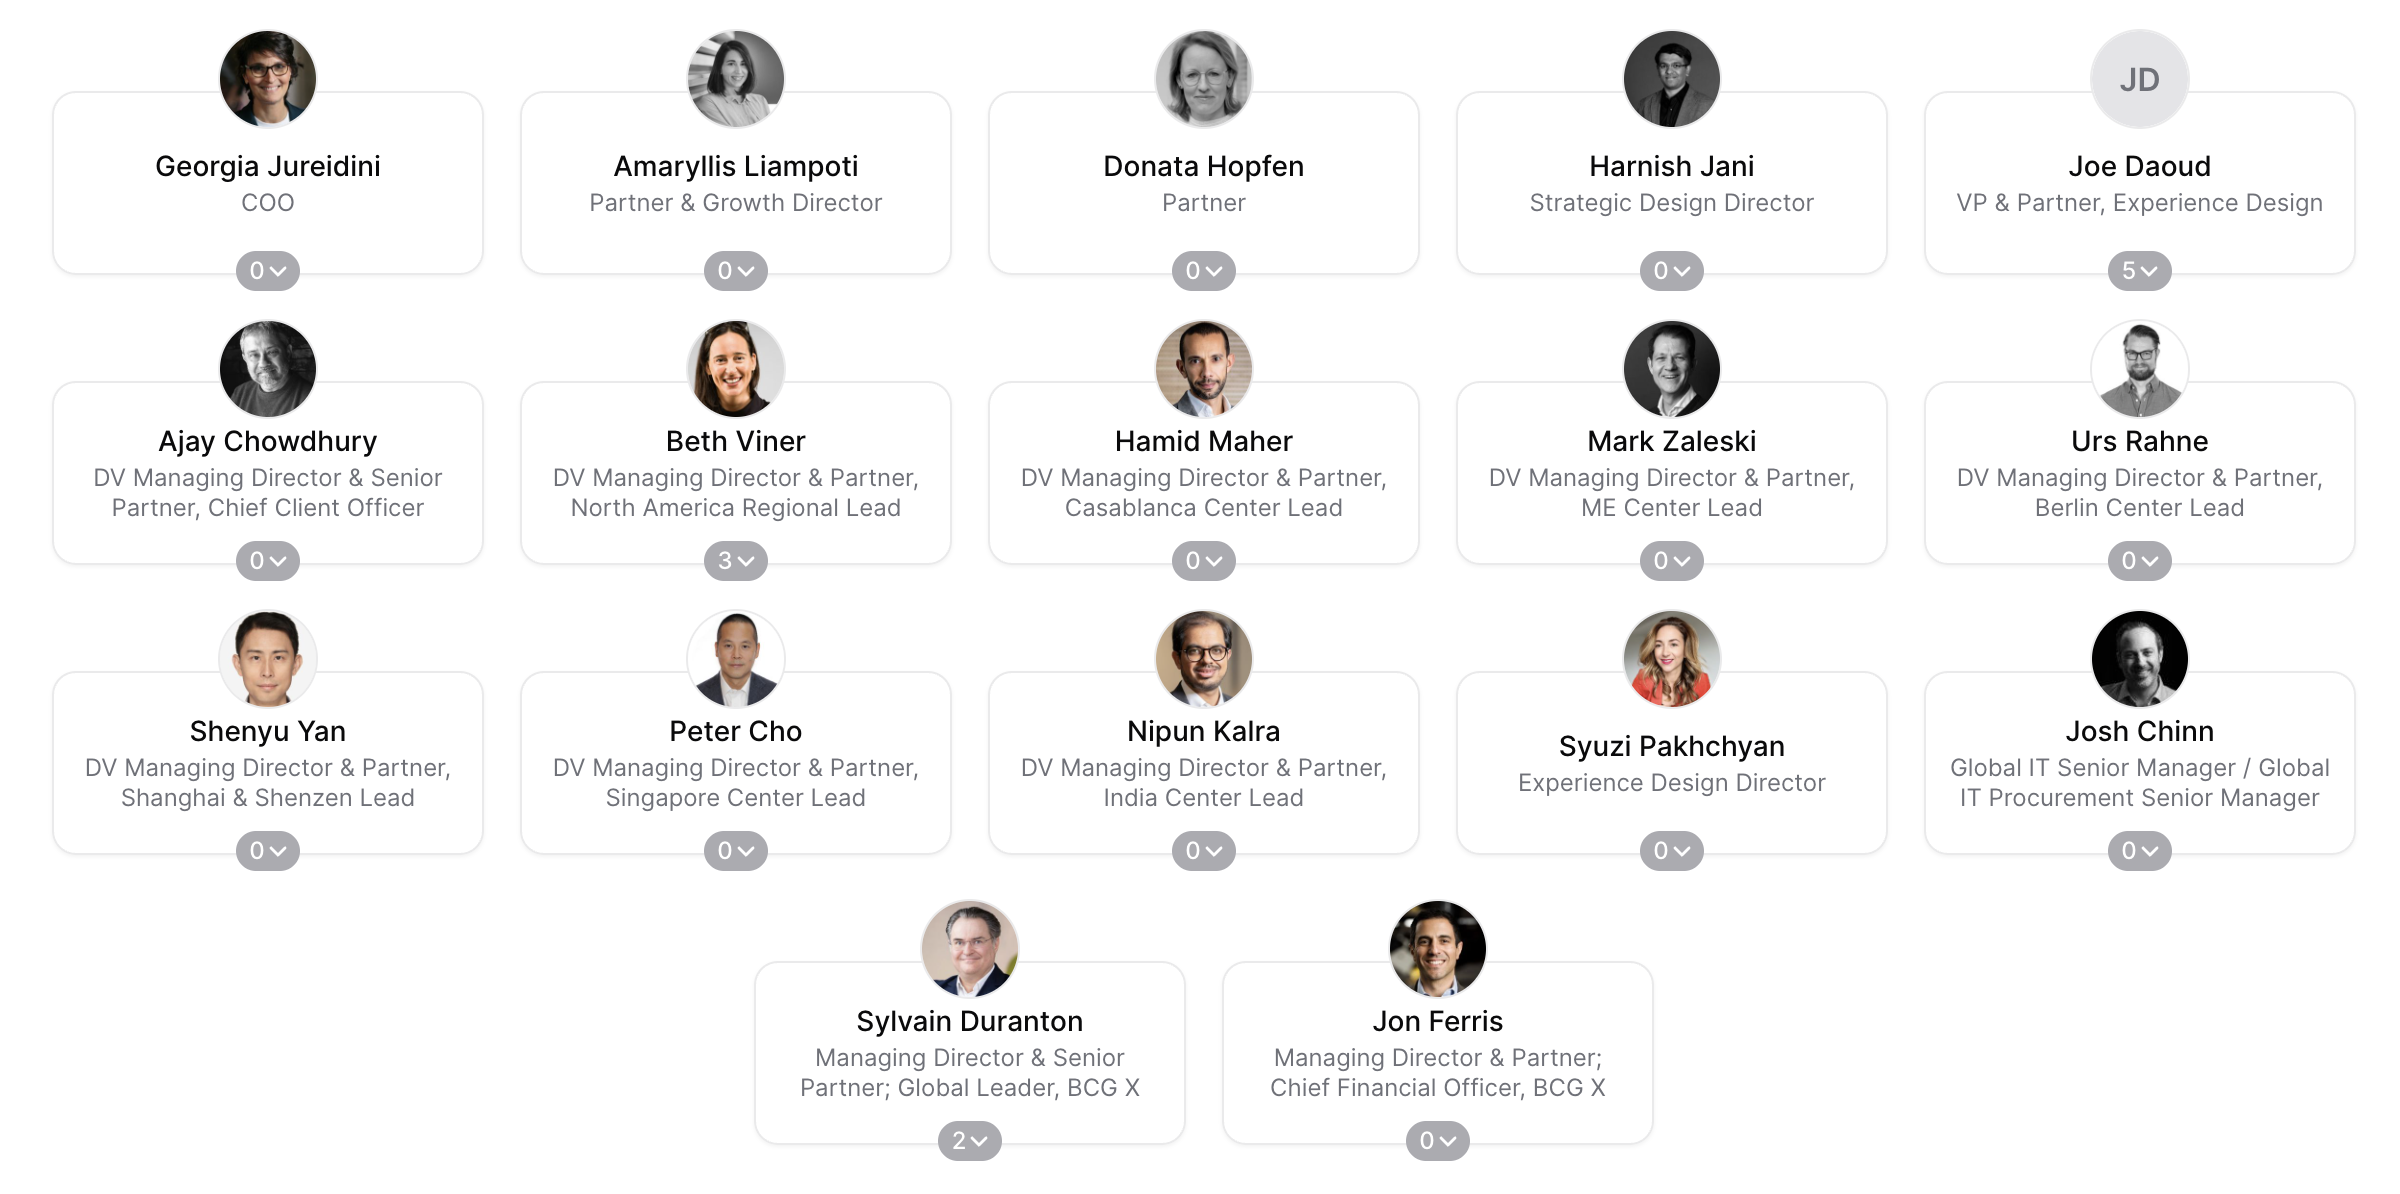
\includegraphics[width=\linewidth]{Images/Executive Leadership Board.png}
    \captionof{figure}{Executive Leadership Board}\cite{executive_leadership_board}
    \label{fig:executive_leadership_board}
\end{center}
\noindent
\mynewline
BCG X’s organizational design promotes effective decision-making, seamless collaboration across global teams, and responsiveness to client needs, leveraging both hierarchical and regional structures.

% Organizational Culture
\subsection{Organizational Culture}
BCG X fosters a dynamic organizational culture defined by innovation, inclusivity, and entrepreneurial spirit. Its culture encourages team members to embrace challenges, take risks, and collaborate openly to drive transformative solutions for clients.\mynewline

Key aspects of BCG X’s organizational culture include:
\begin{itemize}
    \item \textbf{Innovation and Entrepreneurship }\\
        Innovation is central to BCG X's culture, which consistently emphasizes entrepreneurial mindsets, encouraging individuals to explore new ideas, technologies, and methodologies. Employees are supported in developing digital solutions that significantly impact businesses and industries.
    \item \textbf{Inclusivity and Employee Well-being }\\
        BCG X prioritizes a culture of inclusivity and well-being, providing a supportive environment that values diverse perspectives and encourages personal and professional growth. The organization actively supports employees through wellness programs, career coaching, tuition reimbursement, and structured promotion pathways.
    \item \textbf{Open Communication and Collaboration }\\
        Transparent and open communication is encouraged within the organization, fostering a collaborative environment where ideas can flow freely. Employees are empowered to communicate openly, enabling swift decision-making and fostering strong internal relationships and teamwork.
    \item \textbf{Ambition and Growth Orientation }\\
        The organizational culture at BCG X highly values ambitious, growth-oriented individuals who are comfortable navigating ambiguity and pushing boundaries. This ambition is reflected in rapid innovation cycles, strategic client engagements, and a constant drive to achieve impactful outcomes.
\end{itemize}

Overall, BCG X’s organizational culture underpins its ability to deliver high-impact digital transformation and innovation, driven by motivated, collaborative, and empowered teams.


% Project Framework
\section{Project Framework}

% Agentic AI in Legal Operations
\subsection{Agentic AI in Legal Operations}
Agentic AI refers to a specialized form of Artificial Intelligence designed to autonomously execute tasks and make decisions based on predefined high-level goals, adapting dynamically to changing data and operational contexts. This represents an innovative shift from traditional imperative systems toward more autonomous, goal-oriented decision-making processes. Specifically, in legal operations, Agentic AI significantly improves flexibility, scalability, and efficiency by automating complex workflows traditionally dependent on extensive manual interventions.\mynewline

Within legal applications, Agentic AI provides capabilities such as automated clause selection, intelligent contract data mapping, continuous monitoring, and compliance verification. These autonomous functionalities streamline conventional manual activities involved in contract drafting, validation, and ongoing compliance monitoring, significantly reducing contract processing times while improving accuracy and operational effectiveness.

%Digital Contract Management
\subsection{Digital Contract Management}
The process of contract management traditionally involves manual drafting, iterative feedback loops, and approval workflows that often lead to inefficiencies, errors, and delays. Digital Contract Management (DCM) solutions have emerged to address these issues, aiming to centralize, automate, and optimize the entire lifecycle of contract operations—from initial drafting to final execution and continuous monitoring.\mynewline

DCM employs sophisticated AI-driven agents capable of real-time collaboration, intelligent clause insertion, and automated verification. This approach enhances operational efficiency, reduces manual effort in repetitive tasks, and improves compliance by automatically tracking regulatory changes and adapting contracts accordingly. Digital contract management thus transforms legal operations into agile, scalable, and error-resistant processes, significantly boosting organizational productivity and risk management.

% Need for Intelligent Legal Workflow Systems
\subsection{Need for Intelligent Legal Workflow Systems}
Traditional legal workflows suffer from manual bottlenecks, fragmented processes, and compliance risks due to frequent internal and external regulatory changes. The manual approach limits scalability and visibility, causing significant inefficiencies in managing contractual obligations and deadlines.\mynewline

Implementing Intelligent Legal Workflow Systems, powered by Agentic AI, addresses these pain points by automating repetitive tasks, providing real-time monitoring of contract lifecycles, and offering predictive insights into compliance and risk management. These systems ensure seamless collaboration between various stakeholders, streamline approval processes, and mitigate risks through automated compliance checks. The result is a robust, scalable framework capable of handling complex legal workflows with improved transparency and accountability.

% Problematic
\subsection{Problematic}
Current contract management and legal operations rely heavily on manual inputs, iterative feedback loops, and scattered stakeholder communications, leading to inefficiencies, compliance risks, and delays. Contract drafting and validation processes are especially impacted, often resulting in lengthy negotiation cycles, limited visibility into contract deadlines, and difficulty in ensuring consistent regulatory compliance across different jurisdictions. The lack of automated systems further exacerbates these issues, causing increased operational costs and elevated risk profiles.

% Objectives
\subsection{Objectives}
This project aims to deploy and evaluate the effectiveness of an AI-driven intelligent contract management platform leveraging Agentic AI to transform traditional legal operations into streamlined, scalable, and automated processes.\mynewline

The specific objectives include:
\begin{itemize}
    \item Automating repetitive and manual contract drafting tasks through AI pre-filling and intelligent clause selection.
    \item Establishing real-time, AI-driven monitoring and compliance validation of contracts.
    \item Enhancing collaboration and efficiency across multiple stakeholders via automated workflows and digital signatures.
    \item Reducing overall contract processing time and manual effort significantly (40-60\% reduction target).
    \item Minimizing compliance risks through automated regulatory updates and monitoring, aiming for a 30\% risk reduction.
\end{itemize}

Achieving these goals will provide a standardized, scalable solution capable of significantly enhancing efficiency, compliance, and risk management across legal operations.

% Project Management
\section{Project Management}
The project management approach employed during my internship was meticulously structured to ensure smooth execution and timely delivery. Our methodology was grounded in Agile principles, specifically utilizing the Scrum framework to manage the iterative development and deployment of the intelligent contract management platform.

% Scrum Methodology
\subsection{Scrum Methodology}
Scrum is an Agile project management framework designed to facilitate iterative progress through collaboration, flexibility, and responsiveness to feedback. This methodology was particularly suitable for our project due to the dynamic and innovative nature of AI-driven platform development.

\begin{center}
    \centering
    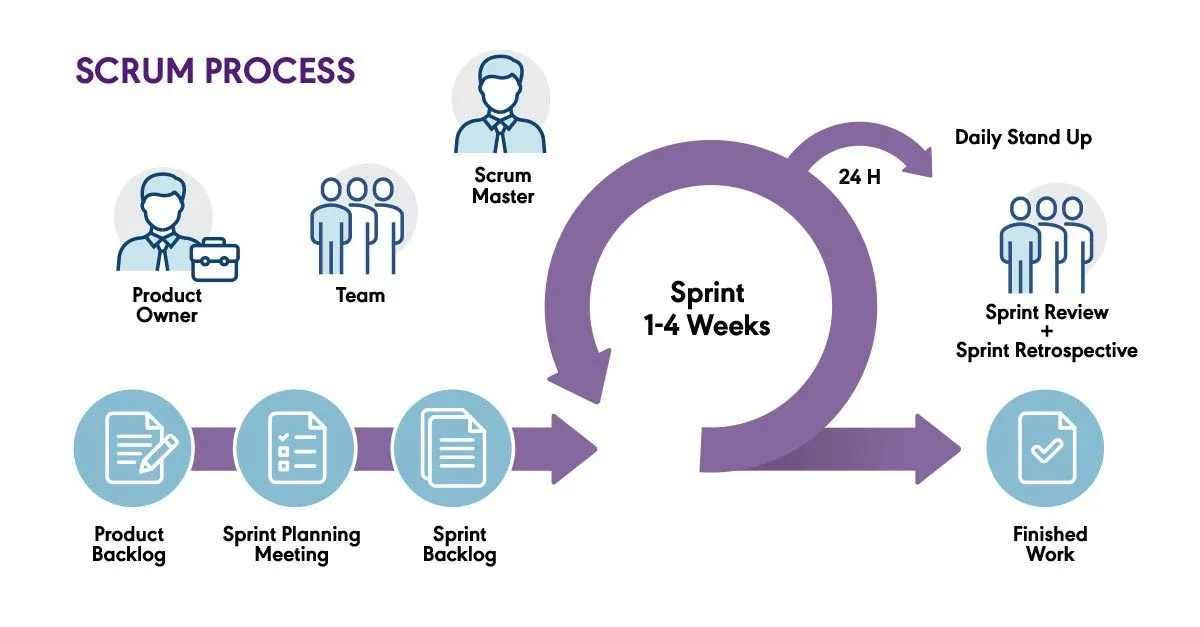
\includegraphics[width=1\textwidth]{Images/Scrum Process.jpeg}
    \captionof{figure}{Scrum Process} \cite{scrum_process}
    \label{fig:scrum_process}
\end{center}

Scrum methodology revolves around iterative cycles called sprints, typically lasting from one to four weeks. Each sprint begins with sprint planning, where tasks are selected from the product backlog to create the sprint backlog. Daily stand-up meetings are held to review progress, address issues, and plan activities for the day. At the end of each sprint, completed work is reviewed in a sprint review meeting, and team performance is analyzed in a sprint retrospective to continually refine processes and improve productivity.

% Scrum Roles and Responsibilities
\subsubsection{Scrum Roles and Responsibilities}
The Scrum framework clearly defines the roles and responsibilities within the team, enhancing clarity and collaboration:

\begin{itemize}
    \item \textbf{Product Owner}: Defined the project vision, managed the product backlog, and prioritized tasks ensuring alignment with client expectations and project goals.
    \item \textbf{Scrum Master (Project Lead)}: Facilitated daily standups, sprint planning, reviews, and retrospectives; ensured adherence to Agile principles; and resolved any impediments affecting progress.
    \item \textbf{Development Team}: Included software engineers, UX designers, product specialists, and interns who executed the technical, product, and design tasks outlined in each sprint. As an intern, I actively contributed as a member of this development team, participating in software development, integration of AI components, and collaborative problem-solving during each sprint.
\end{itemize}

% Project Execution
\subsection{Project Execution}
The project's lifecycle was divided into incremental and iterative phases (Scoping, Alpha, Beta, Minimum Lovable Product), each strategically managed through one-to-two-week sprints. Each sprint encompassed phases of research, design, implementation, testing, and deployment.

% Sprint Structure
\subsubsection{Sprint Structure}
The typical sprint structure adopted for the project was as follows:
\begin{itemize}
    \item \textbf{Sprint Planning}: Tasks were clearly defined and prioritized based on their impact and feasibility.
    \item \textbf{Daily Standups}: Conducted daily for 15 minutes, these sessions updated progress, identified blockers, and adjusted tasks as needed.
    \item \textbf{Weekly Demos}: One-hour weekly meetings where implemented features were demonstrated, allowing stakeholders to review progress, provide feedback, and realign future tasks accordingly.
    \item \textbf{Sprint Review and Retrospective}: Held at the end of each sprint to evaluate completed work, discuss improvements, and refine upcoming tasks.
\end{itemize}

% Meetings and Communication
\subsubsection{Meetings and Communication}
Regular meetings and structured communication were crucial to maintaining project momentum and addressing challenges promptly:

\begin{itemize}
    \item \textbf{Steering Committee (SteerCo)}: Held every two to three weeks, these strategic meetings, involving leadership from BCG and the client, focused on validating use cases, reviewing project approaches, and aligning on vision and roadmap.
    \item \textbf{Weekly Demos}: Facilitated regular feedback loops involving product owners, business analysts, development teams, and client representatives to ensure alignment and adapt quickly to feedback and evolving requirements.
    \item \textbf{Ad-Hoc Sessions}: Dedicated weekly time to address emergent challenges, conduct user testing, validate product iterations, and ensure continuous alignment with legal and regulatory frameworks.
\end{itemize}

% Collaboration Tools
\subsection{Collaboration Tools}
Our team utilized various collaborative and productivity-enhancing tools, significantly streamlining communication, documentation, and project management:

\begin{itemize}
    \item \textbf{ClickUp}: Functioned as the central hub for managing diverse project activities including sprint planning, task assignment, documentation storage, issue tracking, and progress monitoring. It facilitated comprehensive documentation through organized folders for engineering, product, and design documentation, as well as centralized spaces for meeting notes and general project insights.
\end{itemize}

\begin{center}
    \centering
    
\includegraphics[width=0.2\textwidth]{Images/ClickUp Logo.jpeg}
    \captionof{figure}{ClickUp Logo} \cite{clickup_logo}
    \label{fig:clickup_logo}
\end{center}

\begin{itemize}
    \item \textbf{Slack}: Facilitated instant communication and collaboration among team members, enabling quick discussions and efficient problem-solving.
\end{itemize}

\begin{center}
    \centering
    
\includegraphics[width=0.2\textwidth]{Images/Slack Logo.png}
    \captionof{figure}{Slack Logo} \cite{slack_logo}
    \label{fig:slack_logo}
\end{center}

\begin{itemize}
    \item \textbf{Zoom and Microsoft Teams}: Used extensively for virtual meetings, sprint demos, and daily standups, providing robust audio-visual communication capabilities.
\end{itemize}

\begin{center}
    \centering
    
\includegraphics[width=0.4\textwidth]{Images/Zoom and Microsoft Teams Logos.png}
    \captionof{figure}{Zoom and Microsoft Teams Logos} \cite{zoom_logo} - \cite{microsoft_teams_logo}
    \label{fig:zoom_and_microsoft_teams_logos}
\end{center}

\begin{itemize}
    \item \textbf{Microsoft Outlook}: Managed meetings, reminders, and task scheduling, ensuring structured daily and weekly routines.
\end{itemize}

\begin{center}
    \centering
    
\includegraphics[width=0.2\textwidth]{Images/Microsoft Outlook Logo.png}
    \captionof{figure}{Microsoft Outlook Logo} \cite{microsoft_outlook_logo}
    \label{fig:microsoft_outlook_logo}
\end{center}

\begin{itemize}
    \item \textbf{Miro}: Supported visual collaboration, particularly useful during ideation, design sessions, and feedback workshops.
\end{itemize}

\begin{center}
    \centering
    
\includegraphics[width=0.2\textwidth]{Images/Miro Logo.png}
    \captionof{figure}{Miro Logo} \cite{miro_logo}
    \label{fig:miro_logo}
\end{center}

% Project Timeline and Milestones
\subsection{Project Timeline and Milestones}
The project followed a clearly structured roadmap divided into four primary phases, each critical for incremental delivery and validation:

\begin{itemize}
    \item \textbf{Scoping \& Tech Foundations (Weeks 1-3)}: Defined objectives, system design, and initial architecture.
    \item \textbf{Alpha Build (Weeks 3-9)}: Developed the first operational version, enabling preliminary testing and stakeholder feedback.
    \item \textbf{Beta Build (Weeks 9-15)}: Refined the product based on real-world usage, addressing user feedback and enhancing system reliability.
    \item \textbf{Minimum Lovable Product (Weeks 15-21)}: Delivered an enterprise-grade, production-ready platform.
\end{itemize}

This structured and iterative management approach, supported by Agile Scrum methodologies and robust tool usage, enabled our team to effectively respond to changing requirements, maintain alignment with project objectives, and deliver a comprehensive, innovative solution tailored to enhancing efficiency and compliance in legal operations.


\section{Conclusion}
This chapter introduced BCG and BCG X, framed the project’s objectives around Agentic AI for legal workflows, and described the Agile-based management approach. It laid the groundwork for the technical analysis presented in the next chapter.
\minitoc
\label{Chpt:1}
\clearpage


%%%%%%%%%%%%%%%%%%%%%%%%%%%%%%%%%%%%%
%%%%%   Chapitre 2          %%%%%%%%%
%%%%%%%%%%%%%%%%%%%%%%%%%%%%%%%%%%%%%
\chapter{Analysis and Specifications}
This chapter presents the technical analysis and specifications underlying the contract management solution. It starts with a benchmark of existing tools and justifies the choice of an Agentic AI-based approach. Then, it reviews the core technologies used, including LLMs, LangChain, and LangGraph. The integration of Langfuse and Tiptap is also introduced. Lastly, the chapter details the system’s functional and non-functional requirements.

\newpage
\fancyhead[R]{\textsc{Chapter 2 - Analysis and Specifications}}
\hypertarget{secondchapter}{}
\section{Comparative Analysis}

This section benchmarks existing contract management and legal automation platforms to highlight their features, strengths, and limitations, providing the rationale for developing our specialized Agentic AI solution.

%% Benchmarking Existing Solutions
\subsection{Benchmarking Existing Solutions}
To evaluate the landscape of intelligent contract management platforms, we analyzed three prominent solutions: PandaDoc, Harvey AI, and DocDraft. Each platform was selected specifically for its focus on contract management and legal automation capabilities.

% PandaDoc
\subsubsection{PandaDoc}
PandaDoc is a comprehensive document automation platform designed to streamline the creation, approval, and management of digital documents, including contracts, proposals, and quotes.\mynewline

\begin{center}
    \centering
    
\includegraphics[width=0.3\textwidth]{Images/PandaDoc_logo.png}
    \captionof{figure}{PandaDoc Logo} \cite{pandadoc_logo}
    \label{fig:pandadoc_logo}
\end{center}

Here are the key features of PandaDoc:
\begin{itemize}
    \item \textbf{Dynamic Contract Templates}: Create and manage reusable templates to ensure consistency and efficiency in document creation.
    \item \textbf{Integrated eSignatures}: Facilitate secure and legally binding electronic signatures within documents. 
    \item \textbf{CRM Integrations}: Seamlessly integrate with platforms like Salesforce and HubSpot to synchronize data and streamline workflows. 
    \item \textbf{Contract Repository}: Centralized storage for contracts, enabling easy access, tracking, and management. 
    \item \textbf{Workflow Automation}: Automate approval processes and notifications to reduce manual intervention and accelerate deal closures. 
\end{itemize}

% Harvey AI
\subsubsection{Harvey AI}
Harvey AI is a generative AI platform designed for legal professionals, enabling advanced legal research, document drafting, and compliance analysis with the support of large language models.\mynewline

\begin{center}
    \centering
    
\includegraphics[width=0.3\textwidth]{Images/harveyai_logo.png}
    \captionof{figure}{Harvey AI Logo} \cite{harveyai_logo}
    \label{fig:harveyai_logo}
\end{center}

Harvey AI’s main functionalities include:
\begin{itemize}
    \item \textbf{AI-Powered Legal Research}: Provides fast, accurate legal research across jurisdictions with references and citations.
    \item \textbf{Document Drafting Automation}: Automates the generation and review of legal documents, reducing time and manual effort.
    \item \textbf{Predictive Analytics}: Leverages historical legal data to forecast case outcomes and support strategic decisions.
    \item \textbf{Secure Document Management}: Ensures safe handling and storage of sensitive legal documents.
    \item \textbf{Customizable AI Models}: Allows tailoring of legal AI agents to specific practice areas, workflows, or jurisdictions.
\end{itemize}

% DocDraftyes
\subsubsection{DocDraft}
DocDraft is an AI-powered contract drafting solution focused on automating the generation, review, and management of legal documents for legal teams and firms.\mynewline

\begin{center}
    \centering
    
\includegraphics[width=0.3\textwidth]{Images/docdraft_logo.png}
    \captionof{figure}{DocDraft Logo} \cite{docdraft_logo}
    \label{fig:docdraft_logo}
\end{center}

DocDraft highlights the following core features:
\begin{itemize}
    \item \textbf{Automated Document Drafting}: Quickly generates contracts and legal documents using intelligent pre-built logic.
    \item \textbf{Clause Library}: Offers a rich repository of standard and customizable clauses for efficient contract assembly.
    \item \textbf{Compliance Checks}: Reviews documents to ensure alignment with relevant laws and regulations.
    \item \textbf{Collaboration Tools}: Enables multiple stakeholders to co-author and comment on documents in real-time.
    \item \textbf{Attorney Matching Service}: Connects users to legal experts for document review and legal consultation.
\end{itemize}

% Comparative Analysis
\subsubsection{Comparative Analysis}
The following table summarizes the key features of the three platforms:\vspace{-0.3cm}

\begin{center}
    \centering
    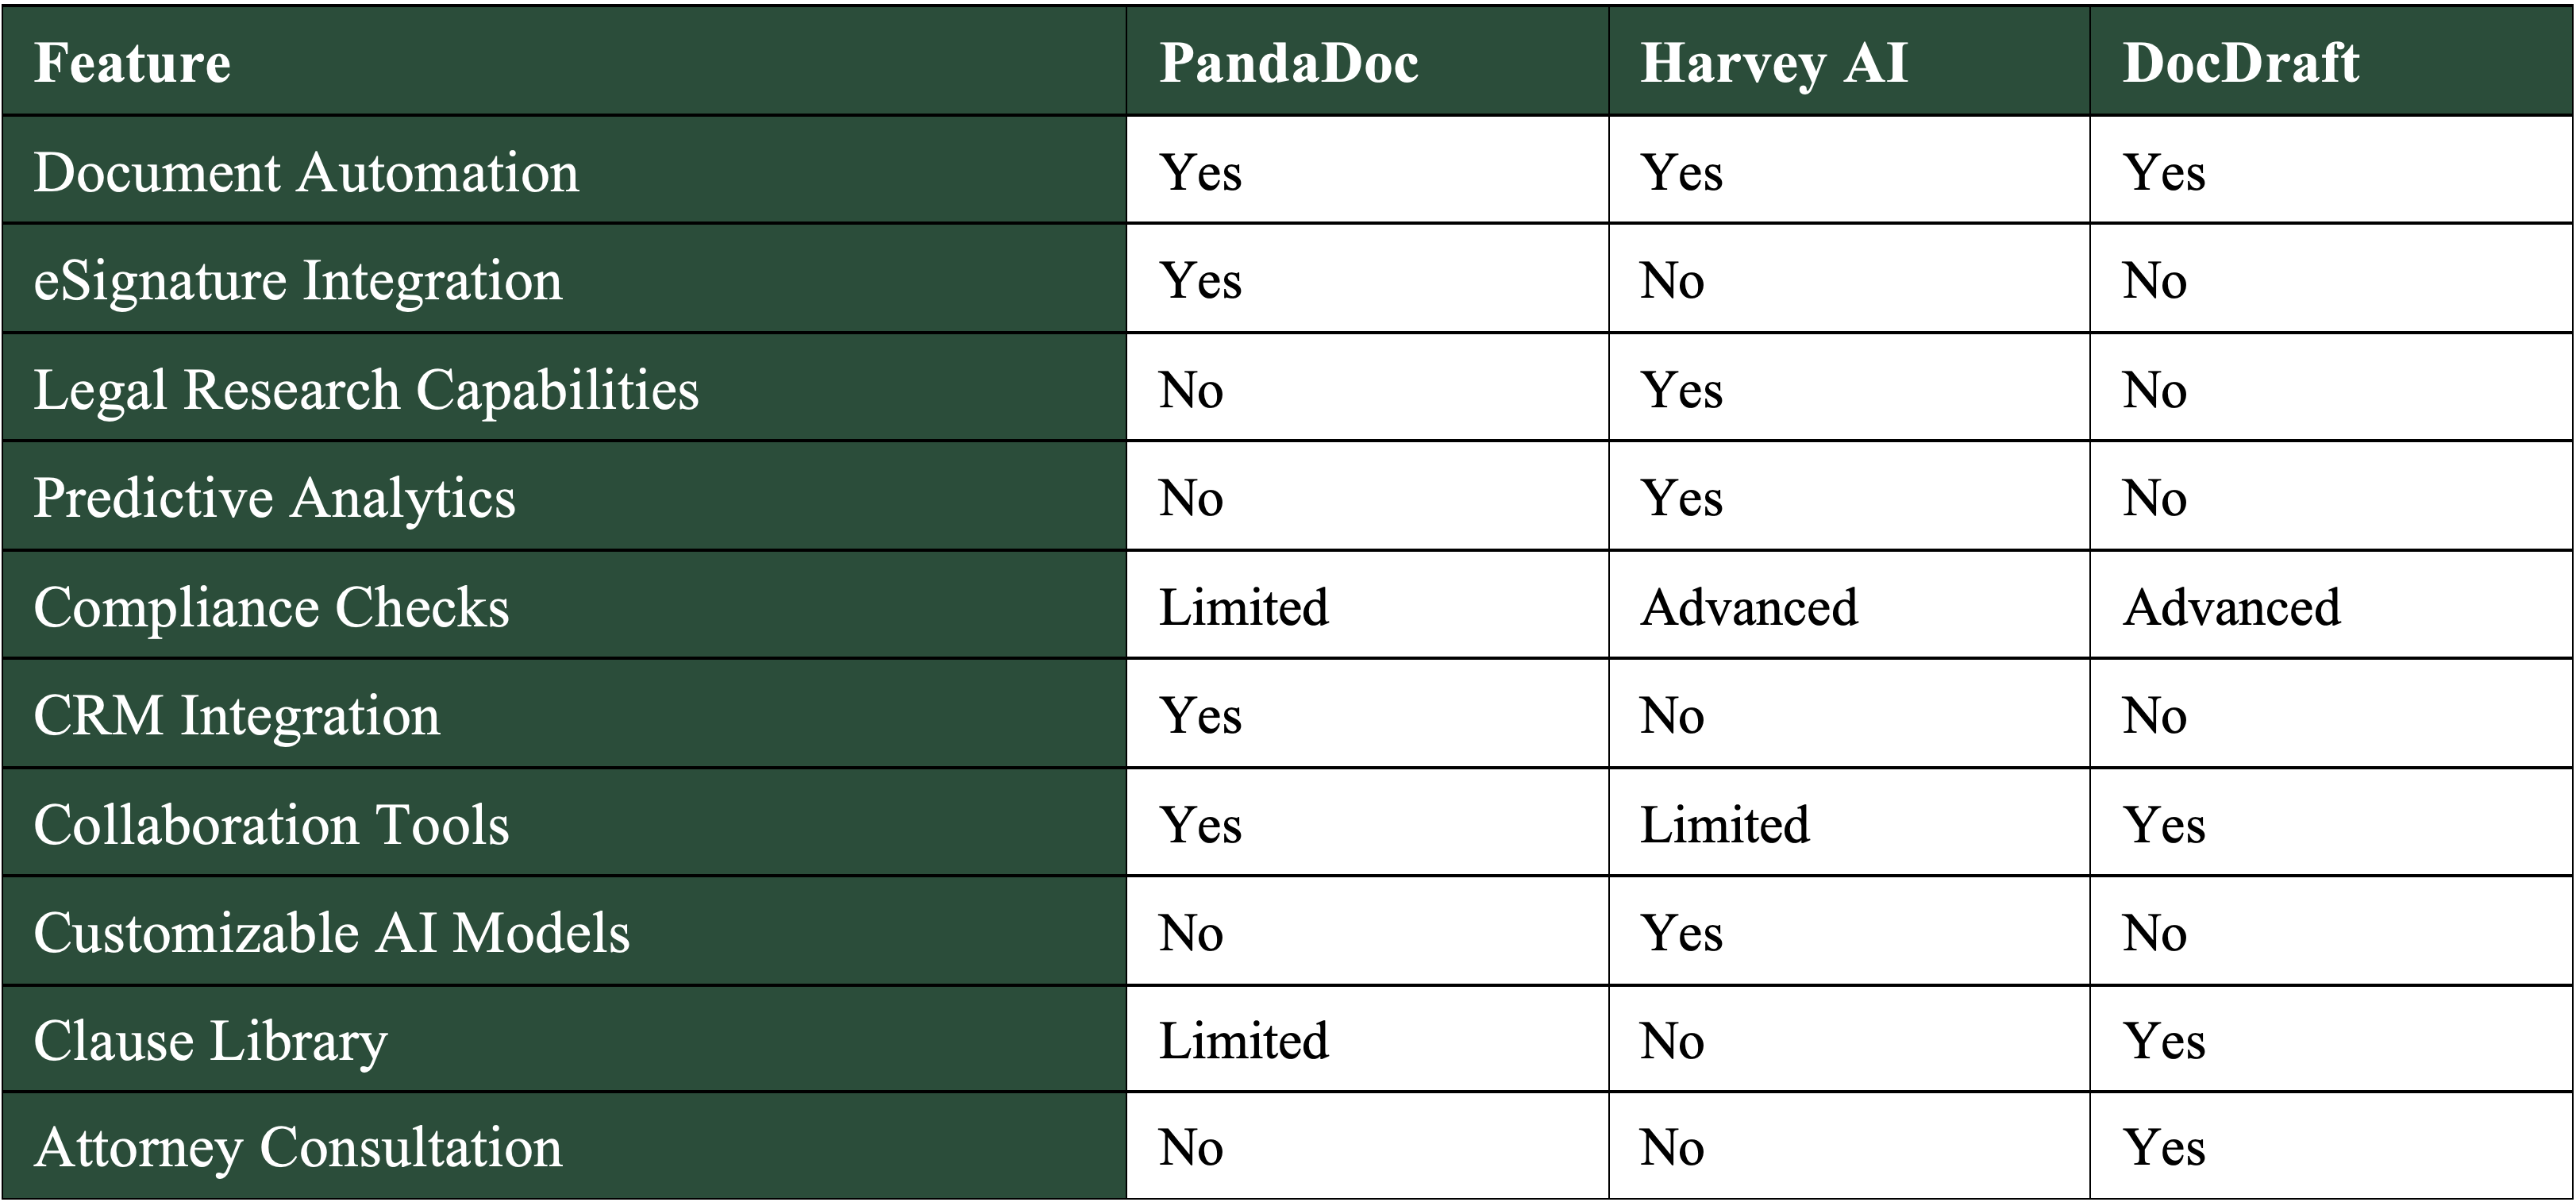
\includegraphics[width=1\textwidth]{Images/Comparison of Contract Management and Legal AI Platforms.png}
    \captionof{table}{Imperative vs. Agentic Approach Comparison}
    \label{tab:comparison_legal_platforms}
\end{center}

% Why We Chose to Build a New Solution
\subsection{Why We Chose to Build a New Solution}
The comparative study clearly revealed that existing contract management platforms were not sufficient to meet our needs. Most tools offer limited automation capabilities and lack the flexibility required for complex legal workflows. Additionally, their inability to support deep integration with enterprise systems, limited orchestration features, and lack of control over agent behavior made them unsuitable for large-scale deployment.\mynewline

To overcome these limitations, we chose to develop a custom solution based on agentic AI. This approach allows us to build a modular, scalable system capable of automating contract drafting, compliance checks, and collaboration, all within a secure and integrated enterprise environment. The goal was not only to improve current processes, but also to lay a solid foundation for future legal automation use cases.\mynewline

To achieve this, we evaluated two principal approaches for building intelligent automation solutions: the traditional imperative approach and the more advanced declarative (agentic) approach. The imperative approach relies on explicit instructions and manual intervention, while the declarative approach leverages autonomous AI agents capable of dynamically adapting to tasks and goals.\mynewline

A detailed comparison of these two methodologies, highlighting the specific advantages of the agentic approach, is presented in Table~\ref{tab:imperative_vs_declarative}. This comparison clearly demonstrates why the agentic (declarative) methodology is more aligned with our requirements and vision, guiding our architectural direction.

\begin{center}
    \centering
    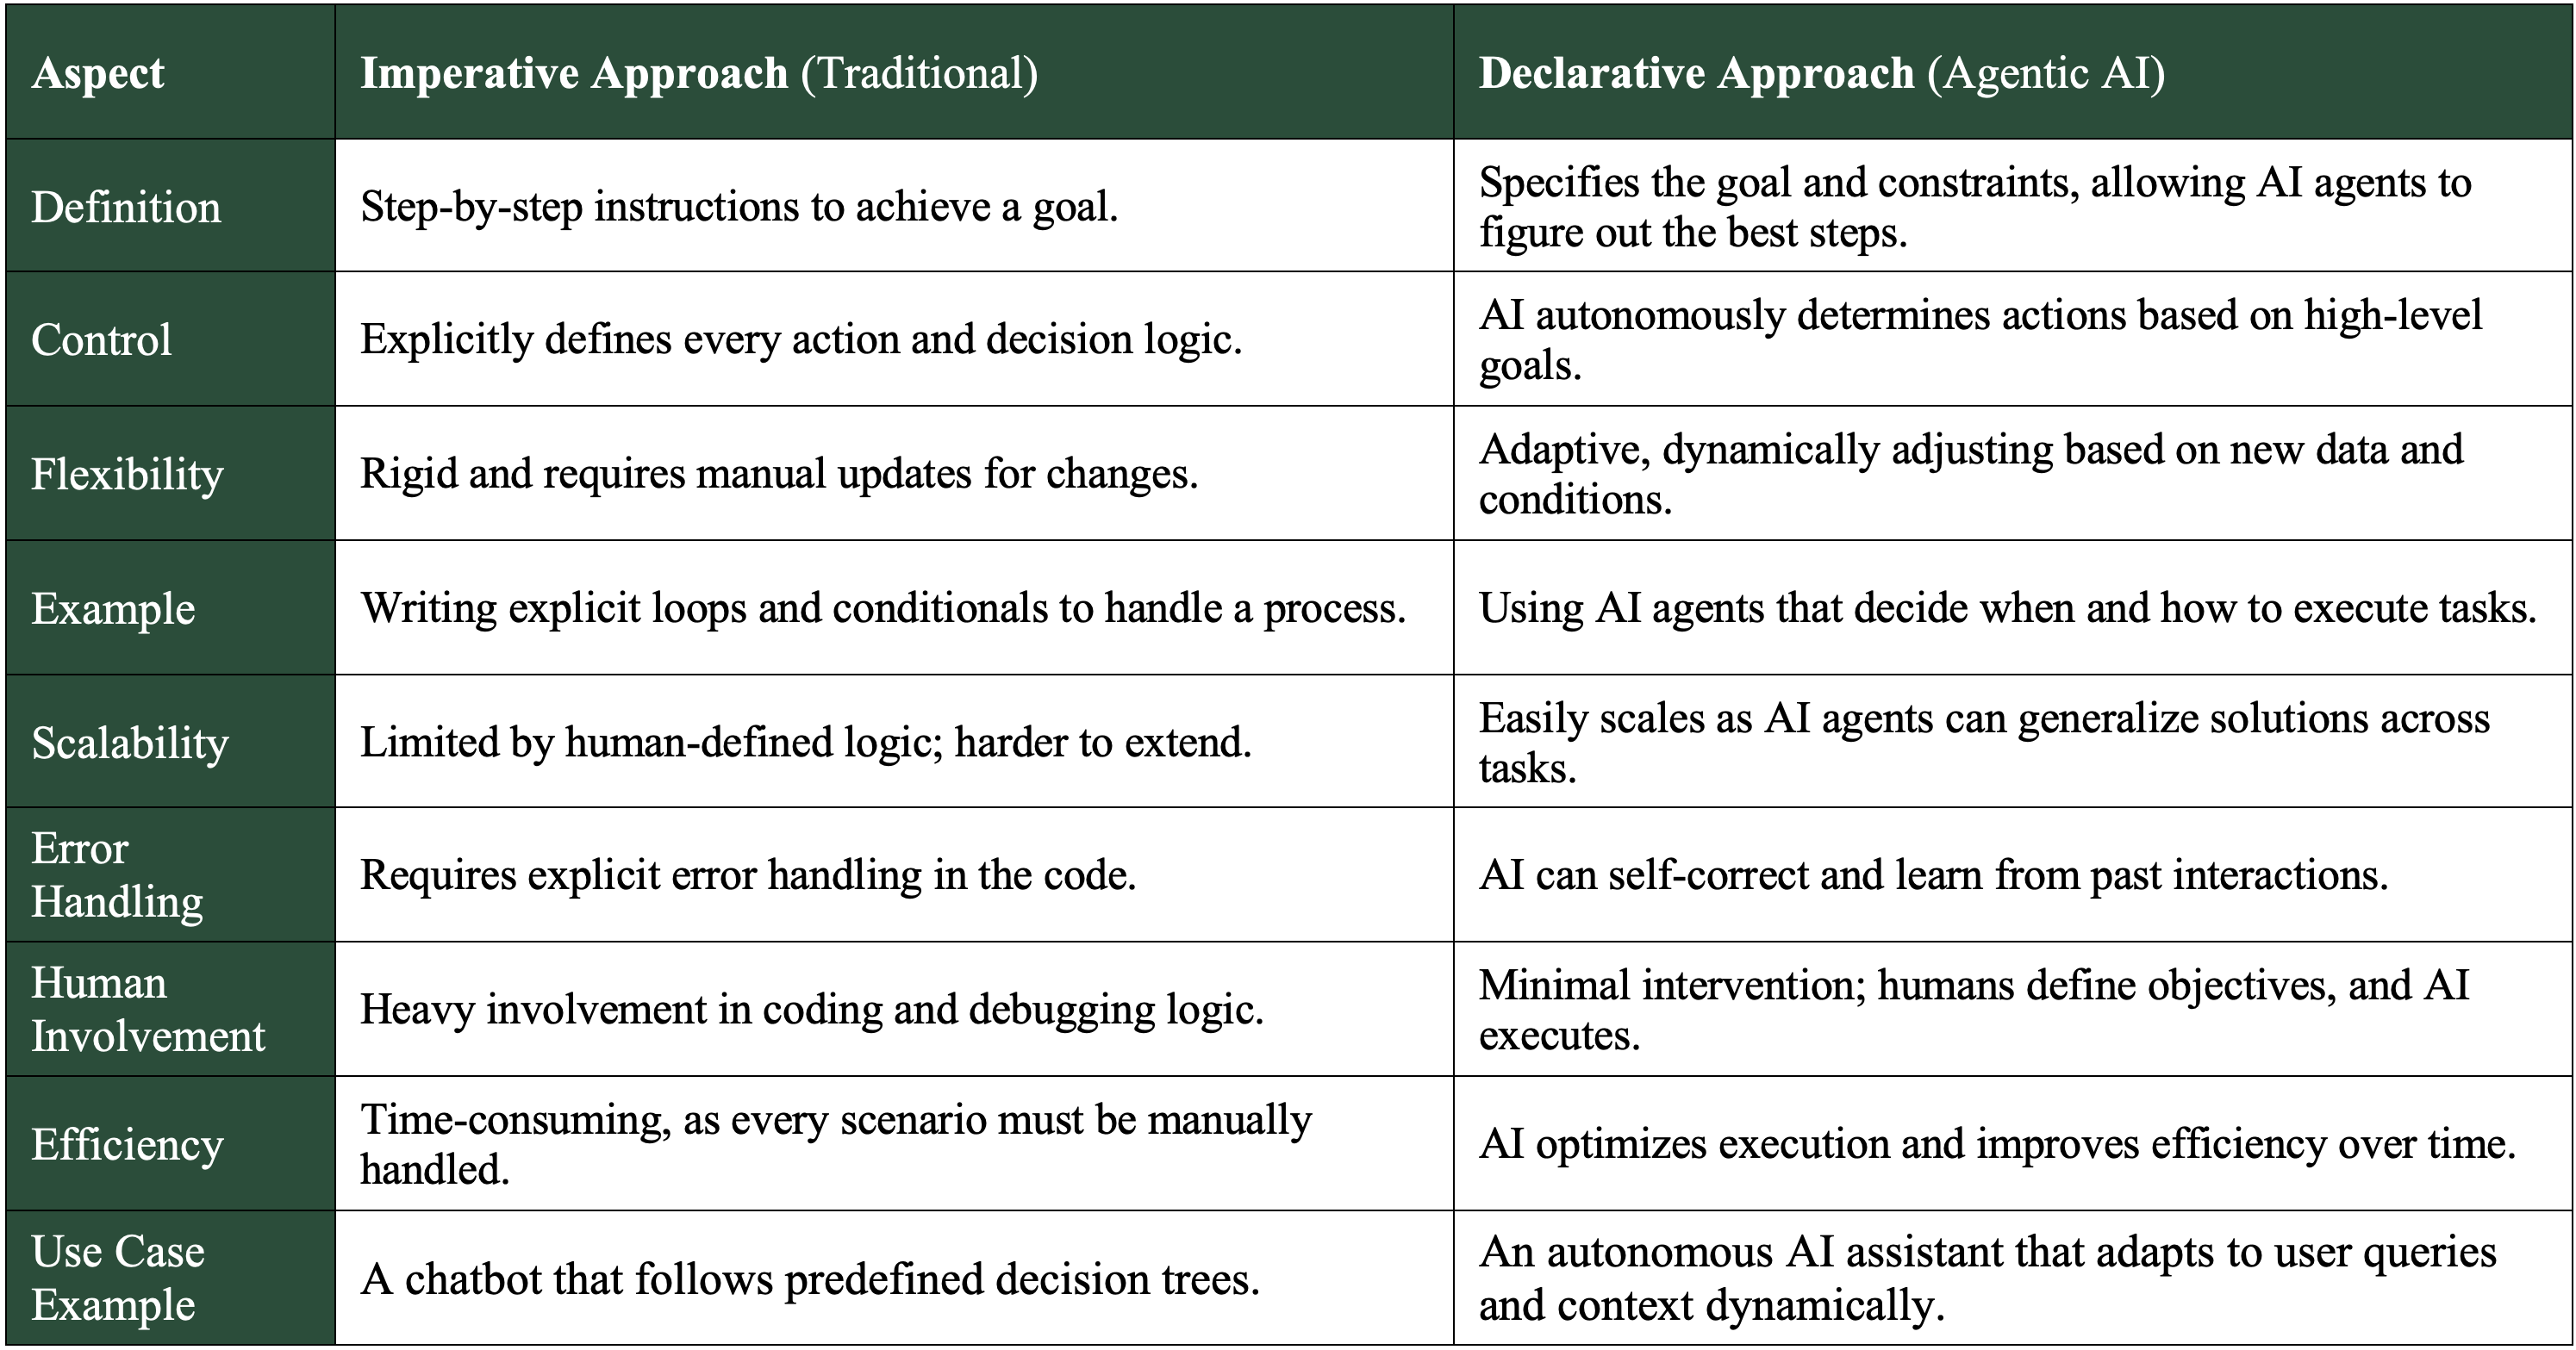
\includegraphics[width=1\textwidth]{Images/Imperative vs. Agentic Approach Comparison.png}
    \captionof{table}{Imperative vs. Agentic Approach Comparison}
    \label{tab:imperative_vs_declarative}
\end{center}


% Technical Background
\section{Technical Background}
This section provides an overview of key technologies enabling the platform's intelligent functionalities.

% Large Language Models (LLMs)
\subsection{Large Language Models (LLMs)}

\subsubsection{Overview}
Large Language Models (LLMs) have revolutionized natural language processing through transformer-based architectures, extensive computational resources, and vast datasets, achieving near-human performance in various linguistic tasks.

\begin{center}
    \centering
    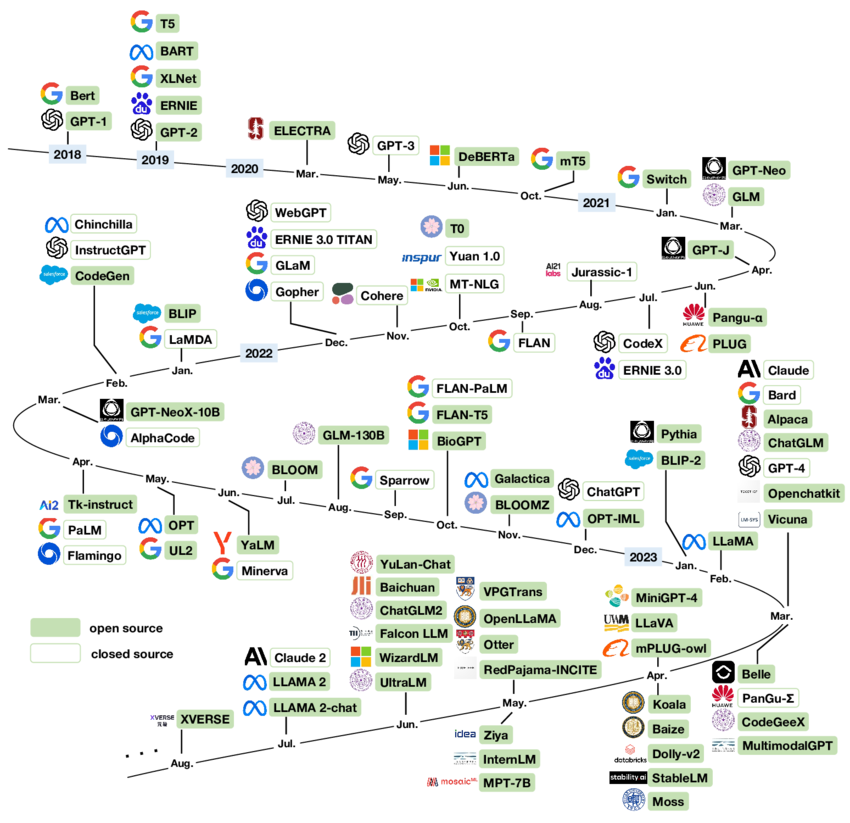
\includegraphics[width=0.9\textwidth]{Images/evolution chronologic LLM.png}
    \captionof{figure}{Chronological Evolution of Large Language Models (LLMs)} \cite{llmEvolution}
    \label{fig:llmEvolution}
\end{center}

\subsubsection{Capabilities and Emergent Properties}
Large Language Models have significantly evolved, exhibiting capabilities such as reasoning, decision-making, and in-context learning, often emerging spontaneously at scale rather than through explicit programming or training. These emergent properties enable LLMs to effectively generalize across diverse tasks without extensive task-specific data, highlighting their robust adaptability. Techniques such as fine-tuning and prompt engineering further enhance model alignment, ensuring outputs align closely with user intents and expectations.\mynewline

LLMs’ adaptability and versatility have found applications in various sectors including healthcare, finance, legal operations, and customer service, underscoring their transformative potential across industries.

\subsubsection{Challenges and Limitations}
Despite these advancements, LLM deployment is constrained by several critical limitations. Key challenges include:

\begin{itemize}
    \item \textbf{Computational Cost and Efficiency}: The resource-intensive nature of LLM training and inference demands considerable computational power, resulting in high operational costs.
    \item \textbf{Input Size Constraints}: Current LLM architectures typically handle context windows of up to 128k tokens, limiting their ability to directly process large-scale data sources comprising millions of tokens.
    \item \textbf{Inference Speed and Latency}: Longer inputs proportionally increase inference time and computational demands, challenging real-time or large-scale applications.
    \item \textbf{Ethical and Bias Considerations}: Models may inadvertently propagate biases present in training data or generate misleading and potentially harmful outputs, necessitating robust ethical oversight.
\end{itemize}

\subsubsection{Future Directions}
Addressing these constraints has become an active area of research. Innovations in model compression techniques, such as pruning, quantization, and distillation, aim to enhance efficiency and accessibility of LLMs. Moreover, emerging architectures and retrieval-augmented generation methods offer promising approaches for handling extensive datasets and large input contexts effectively.

Future advancements are expected to mitigate current limitations, further unlocking the full potential of Large Language Models across diverse, complex applications.

% Agentic AI
\subsection{Agentic AI}

\subsubsection{Overview}
Agentic AI represents a significant evolution in artificial intelligence, transitioning from reactive systems to proactive, autonomous entities capable of setting goals, making decisions, and adapting to dynamic environments. Unlike traditional AI agents that operate within predefined parameters, Agentic AI systems exhibit autonomy, learning, and adaptability, enabling them to handle complex, multi-step tasks with minimal human intervention.

\begin{center}
    \centering
    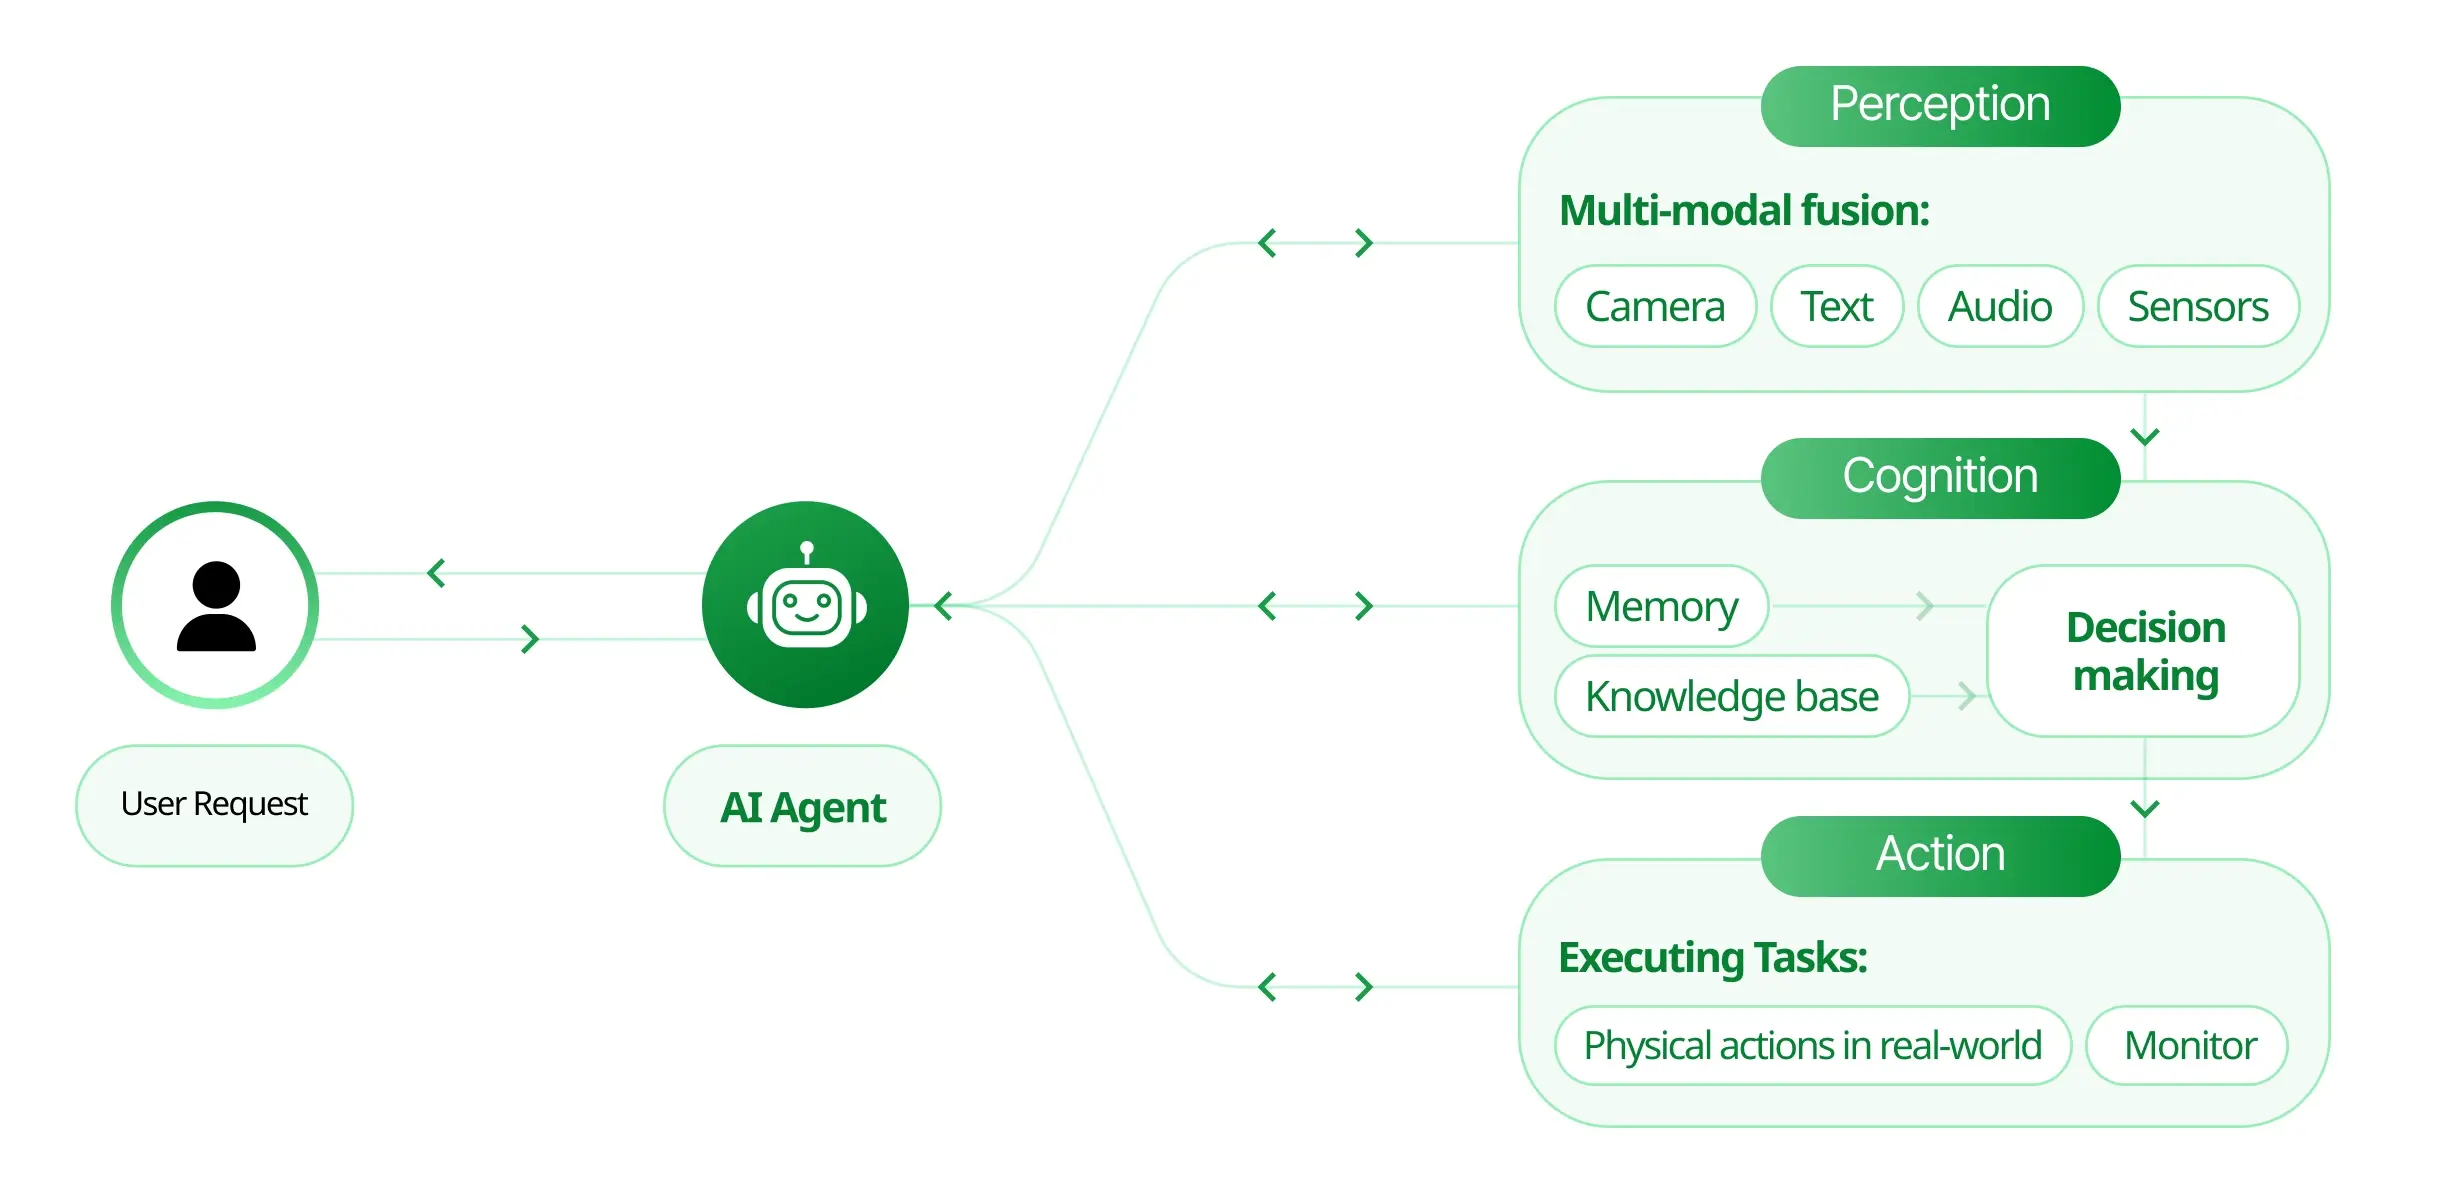
\includegraphics[width=0.9\textwidth]{Images/agentic_ai_architecture.png}
    \captionof{figure}{Agentic AI System Architecture} \cite{agenticAIArchitecture}
    \label{fig:agentic_ai_architecture}
\end{center}

\subsubsection{Core Characteristics}
Agentic AI systems are distinguished by several key features:

\begin{itemize}
    \item \textbf{Autonomy}: They operate independently, making decisions without continuous human oversight.
    \item \textbf{Goal-Oriented Behavior}: These systems can set, pursue, and adjust goals based on environmental feedback.
    \item \textbf{Adaptability}: Agentic AI learns from experiences, refining its strategies to improve performance over time.
    \item \textbf{Complex Decision-Making}: They evaluate multiple options and potential outcomes to make informed decisions.
    \item \textbf{Collaboration}: Agentic AI can coordinate with other agents or systems to achieve shared objectives.
\end{itemize}

\subsubsection{Agentic AI vs. Generative AI}
While both Agentic AI and Generative AI leverage advanced machine learning techniques, their functionalities differ significantly:

\begin{itemize}
    \item \textbf{Generative AI}: Focuses on creating content (text, images, etc.) based on input data, operating primarily in a reactive manner.
    \item \textbf{Agentic AI}: Emphasizes autonomous decision-making and goal pursuit, enabling proactive interactions with the environment.
\end{itemize}

\begin{center}
    \centering
    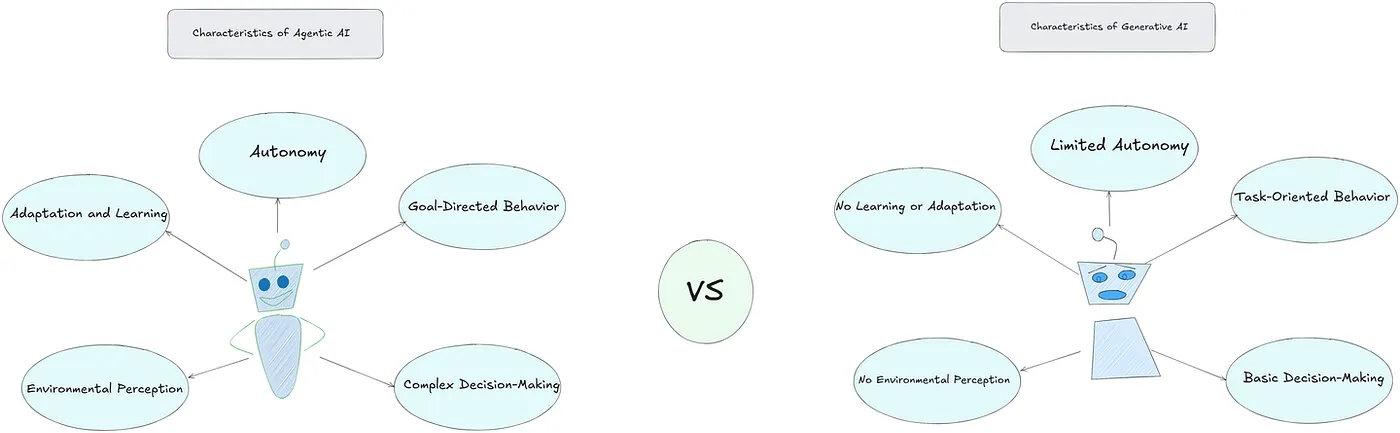
\includegraphics[width=1\textwidth]{Images/agentic_vs_generative_ai.png}
    \captionof{figure}{Comparison Between Agentic AI and Generative AI} \cite{agentic_vs_generative_ai}
    \label{fig:agentic_vs_generative_ai}
\end{center}

\subsubsection{Multi-Agent Systems}
Agentic AI often operates within multi-agent systems, where multiple autonomous agents collaborate to solve complex problems. These systems benefit from:

\begin{itemize}
    \item \textbf{Specialization}: Agents can focus on specific tasks, enhancing efficiency.
    \item \textbf{Scalability}: Systems can be expanded by adding more agents to handle increased complexity.
    \item \textbf{Robustness}: Collaboration among agents can compensate for individual agent failures or limitations.
\end{itemize}

\begin{center}
    \centering
    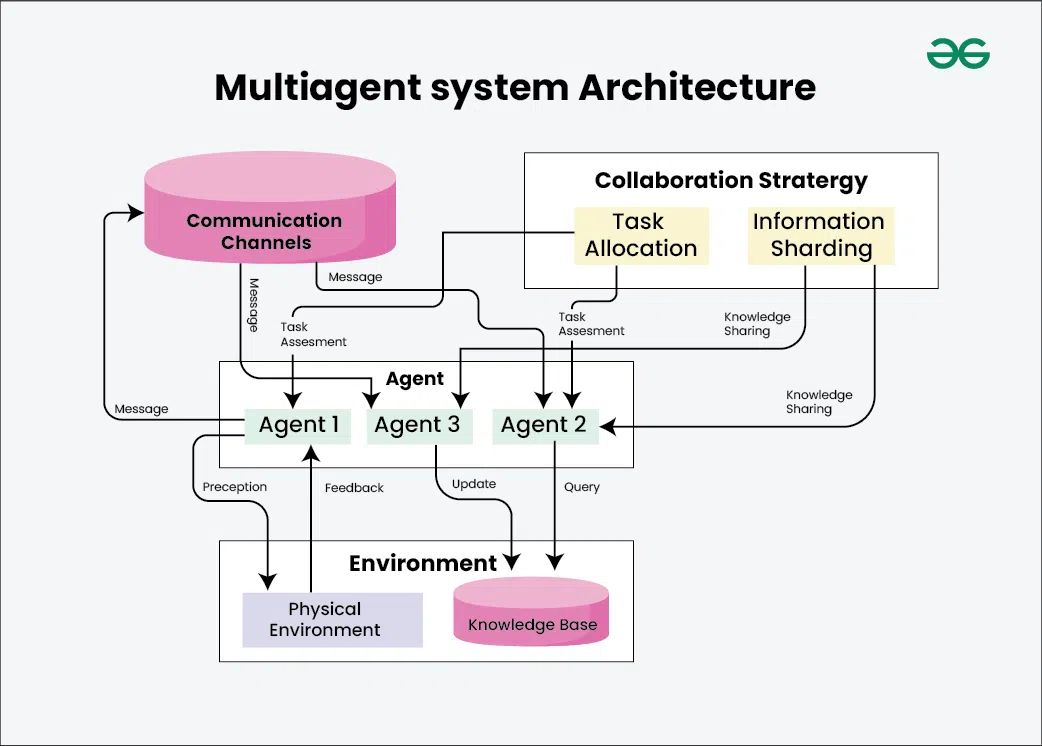
\includegraphics[width=0.9\textwidth]{Images/multi_agent_system.png}
    \captionof{figure}{Multi-Agent System Collaboration} \cite{multi_agent_system}
    \label{fig:multi_agent_system}
\end{center}

\subsubsection{Challenges and Future Directions}
Despite its potential, Agentic AI faces several challenges:

\begin{itemize}
    \item \textbf{Ethical Considerations}: Ensuring decisions align with human values and societal norms.
    \item \textbf{Transparency}: Making decision-making processes understandable to users.
    \item \textbf{Security}: Protecting systems from malicious manipulation or unintended behaviors.
    \item \textbf{Integration}: Seamlessly incorporating Agentic AI into existing infrastructures.
\end{itemize}

Ongoing research aims to address these challenges, focusing on developing frameworks for ethical AI, enhancing interpretability, and establishing standards for safe deployment.

% LangChain and LangGraph
\subsection{LangChain and LangGraph}

\subsubsection{Overview}
LangChain and LangGraph are complementary frameworks designed to facilitate the development of applications powered by Large Language Models (LLMs). While LangChain provides a modular approach to constructing sequential workflows, LangGraph introduces a graph-based paradigm, enabling the creation of complex, dynamic, and stateful AI systems.

\subsubsection{LangChain: Modular Workflow Construction}
LangChain is an open-source framework that simplifies the integration of LLMs into applications by allowing developers to build chains—sequences of calls to LLMs and other utilities. Its modular design supports the composition of various components such as prompt templates, memory modules, and tool integrations. This structure is particularly effective for tasks that follow a linear progression, such as document summarization, question answering, and conversational agents.

\begin{center}
    \centering
    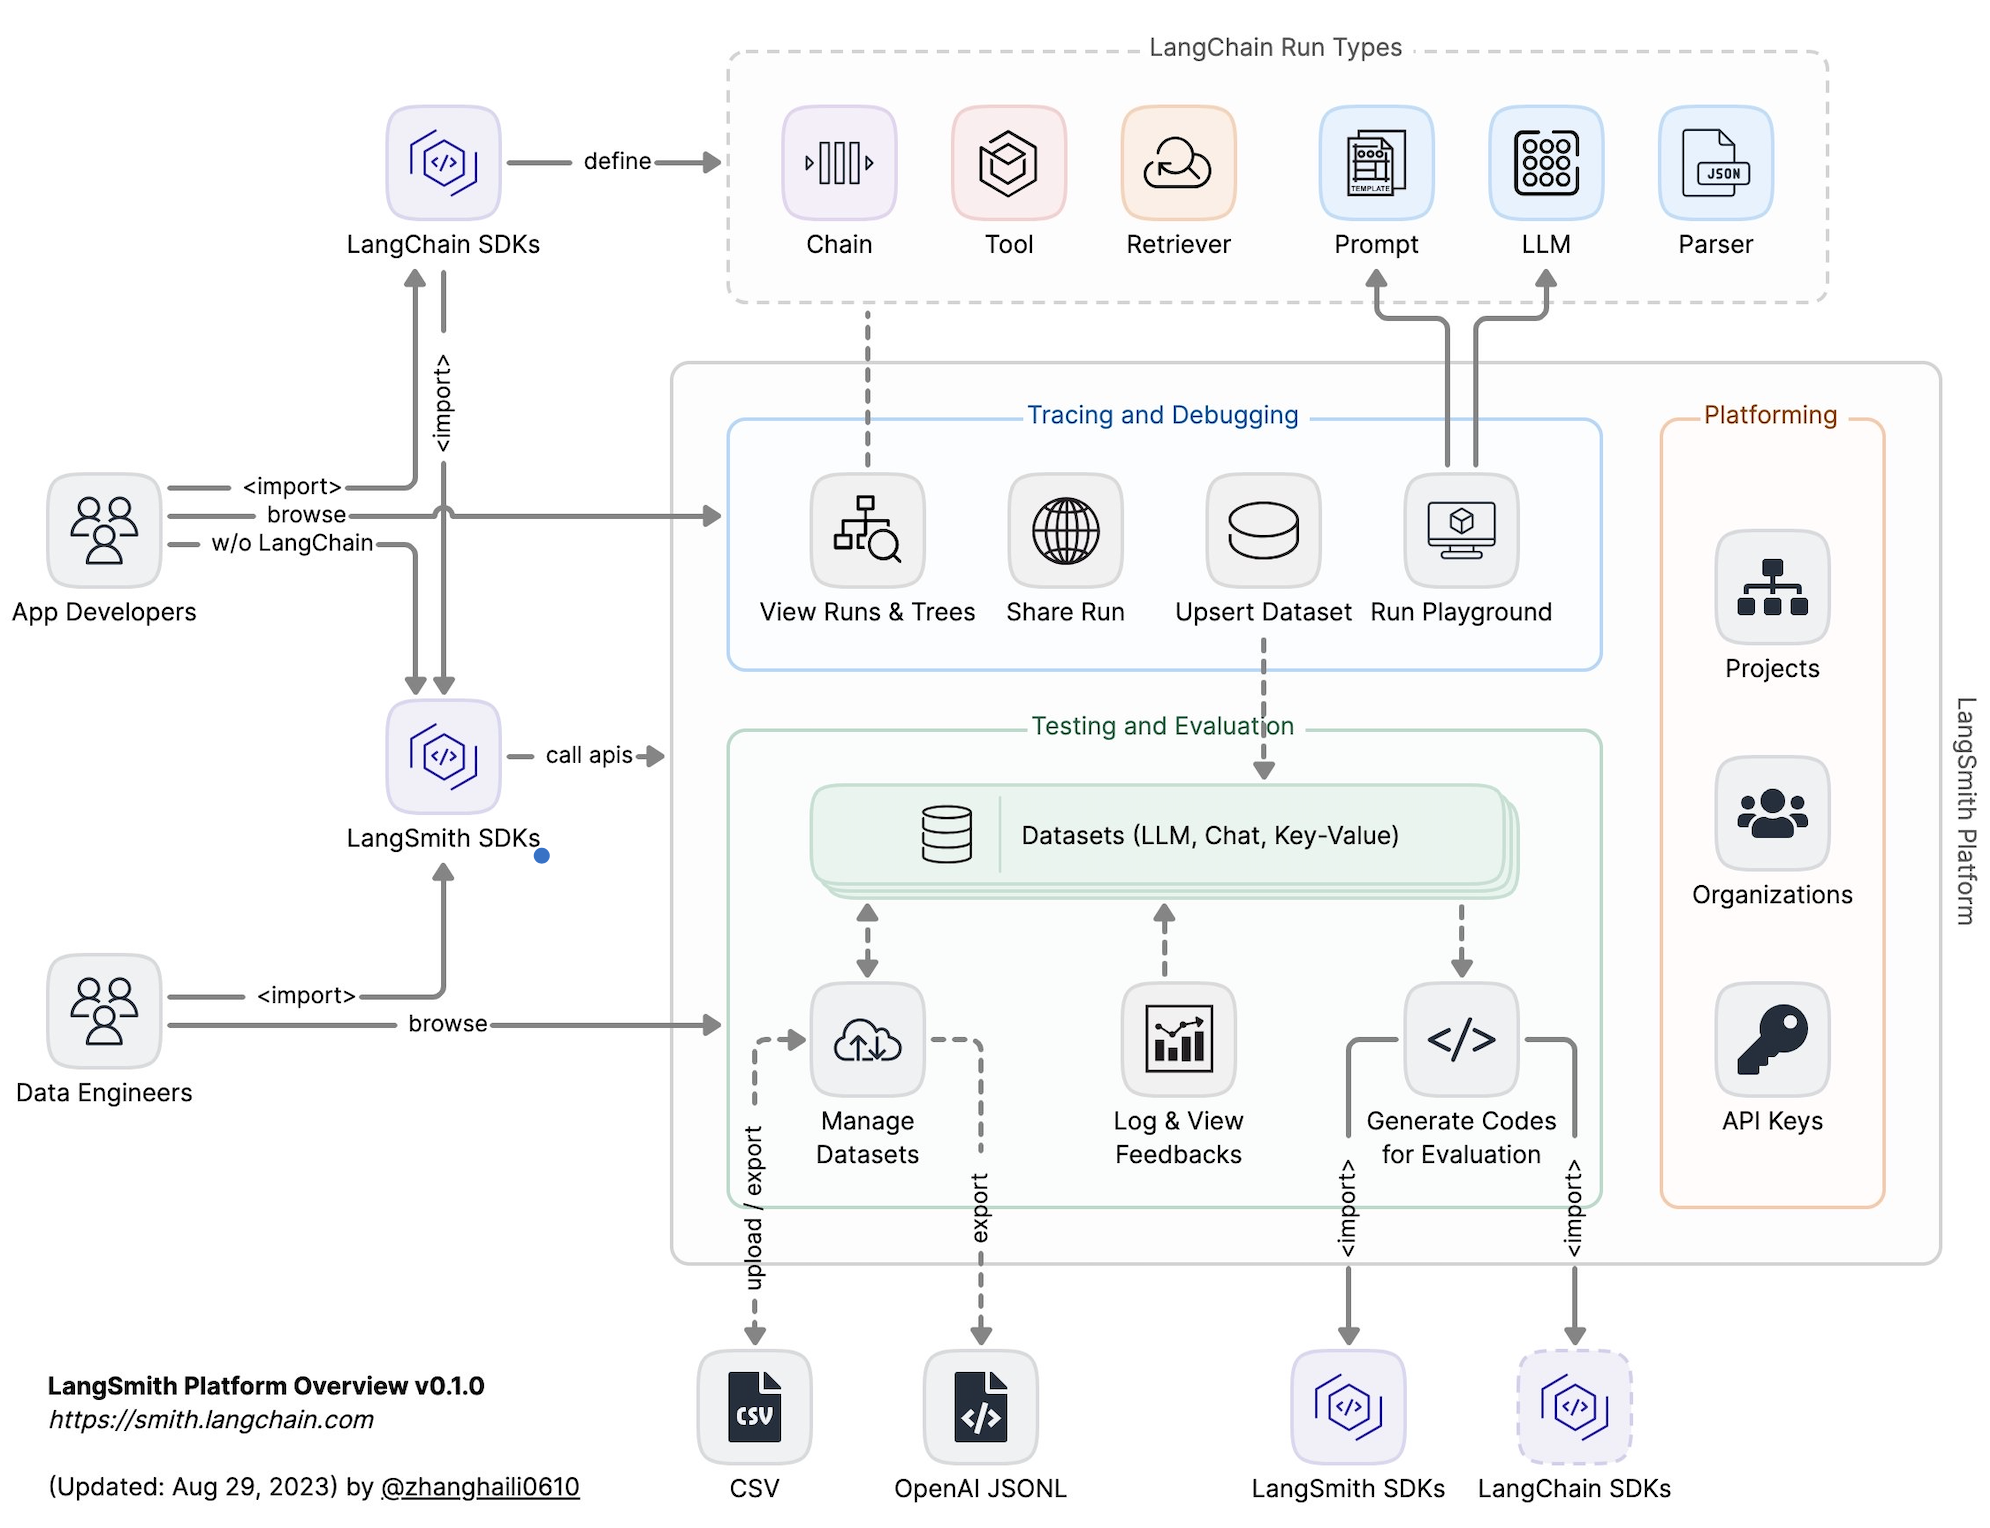
\includegraphics[width=0.9\textwidth]{Images/Langchain Architecture.png}
    \captionof{figure}{LangChain Architecture} \cite{langchainArchitecture}
    \label{fig:langchain_architecture}
\end{center}

Key features of LangChain include:
\begin{itemize}
    \item \textbf{Prompt Templates}: Facilitate the creation of dynamic prompts for LLMs.
    \item \textbf{Chains}: Enable the linking of multiple components to form a cohesive workflow.
    \item \textbf{Agents}: Allow for decision-making capabilities by selecting appropriate actions based on user input.
    \item \textbf{Memory}: Maintain context across interactions to support stateful conversations.
\end{itemize}

\subsubsection{LangGraph: Graph-Based Workflow Orchestration}
Building upon the foundations of LangChain, LangGraph introduces a graph-based approach to workflow orchestration, allowing for the modeling of complex, non-linear, and cyclical processes. In LangGraph, workflows are represented as directed graphs comprising nodes (representing operations or agents) and edges (defining the flow between nodes). This structure is particularly advantageous for applications requiring iterative processing, conditional branching, and multi-agent coordination.

\begin{center}
    \centering
    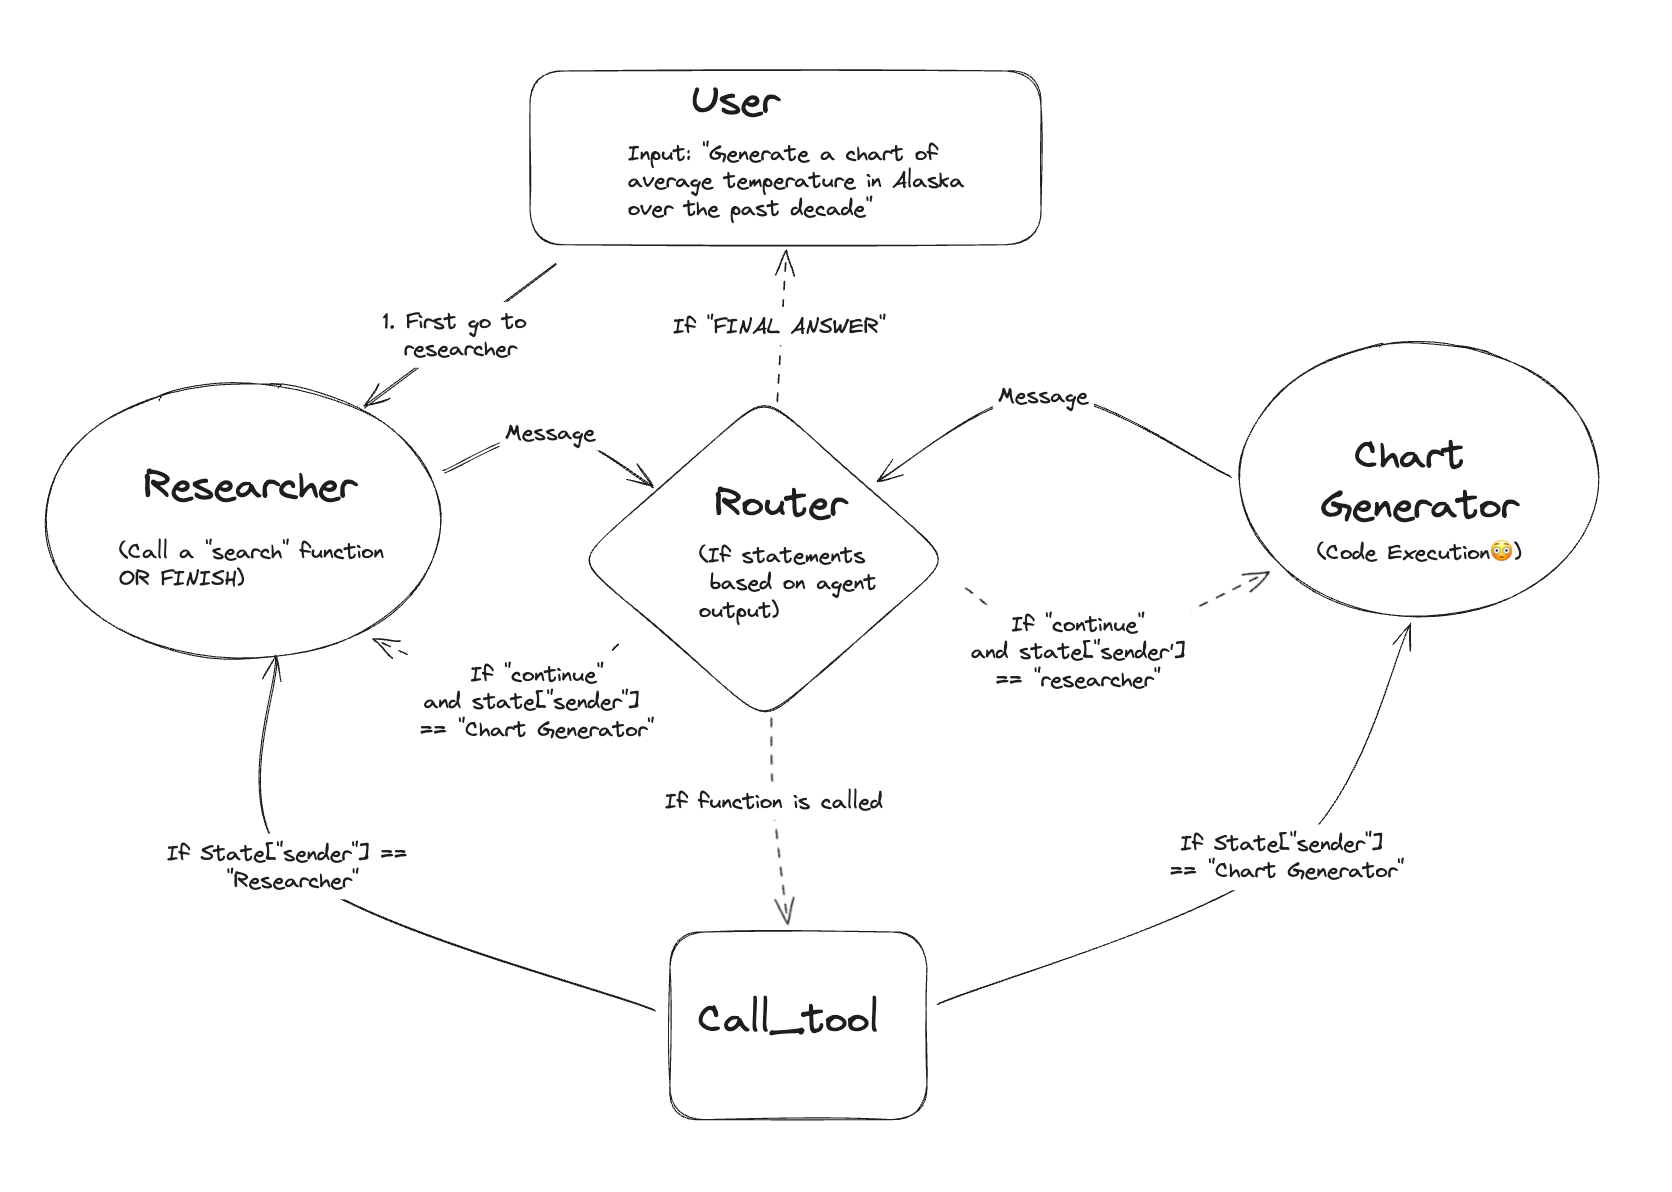
\includegraphics[width=0.9\textwidth]{Images/langgraph_mutil_agent.png}
    \captionof{figure}{LangGraph: Multi-Agent Workflows} \cite{langgraphMultiAgent}
    \label{fig:langgraph_multi_agent}
\end{center}

Notable capabilities of LangGraph include:
\begin{itemize}
    \item \textbf{Cyclic Workflows}: Support for loops and iterative processes within workflows.
    \item \textbf{Conditional Routing}: Dynamic decision-making to determine the next node based on runtime conditions.
    \item \textbf{State Management}: Persistent tracking of the system’s state throughout the workflow execution.
    \item \textbf{Multi-Agent Collaboration}: Facilitation of interactions between multiple agents, each with specialized roles.
\end{itemize}

\subsubsection{Comparative Analysis}
LangChain and LangGraph streamline the development of LLM-powered applications but address varying complexity levels. LangChain is optimal for linear workflows with straightforward tasks and limited iterative processes. In contrast, LangGraph’s dynamic, graph-based structure efficiently manages more intricate workflows involving conditional logic, iterative loops, and robust multi-agent coordination.

\begin{center}
    \centering
    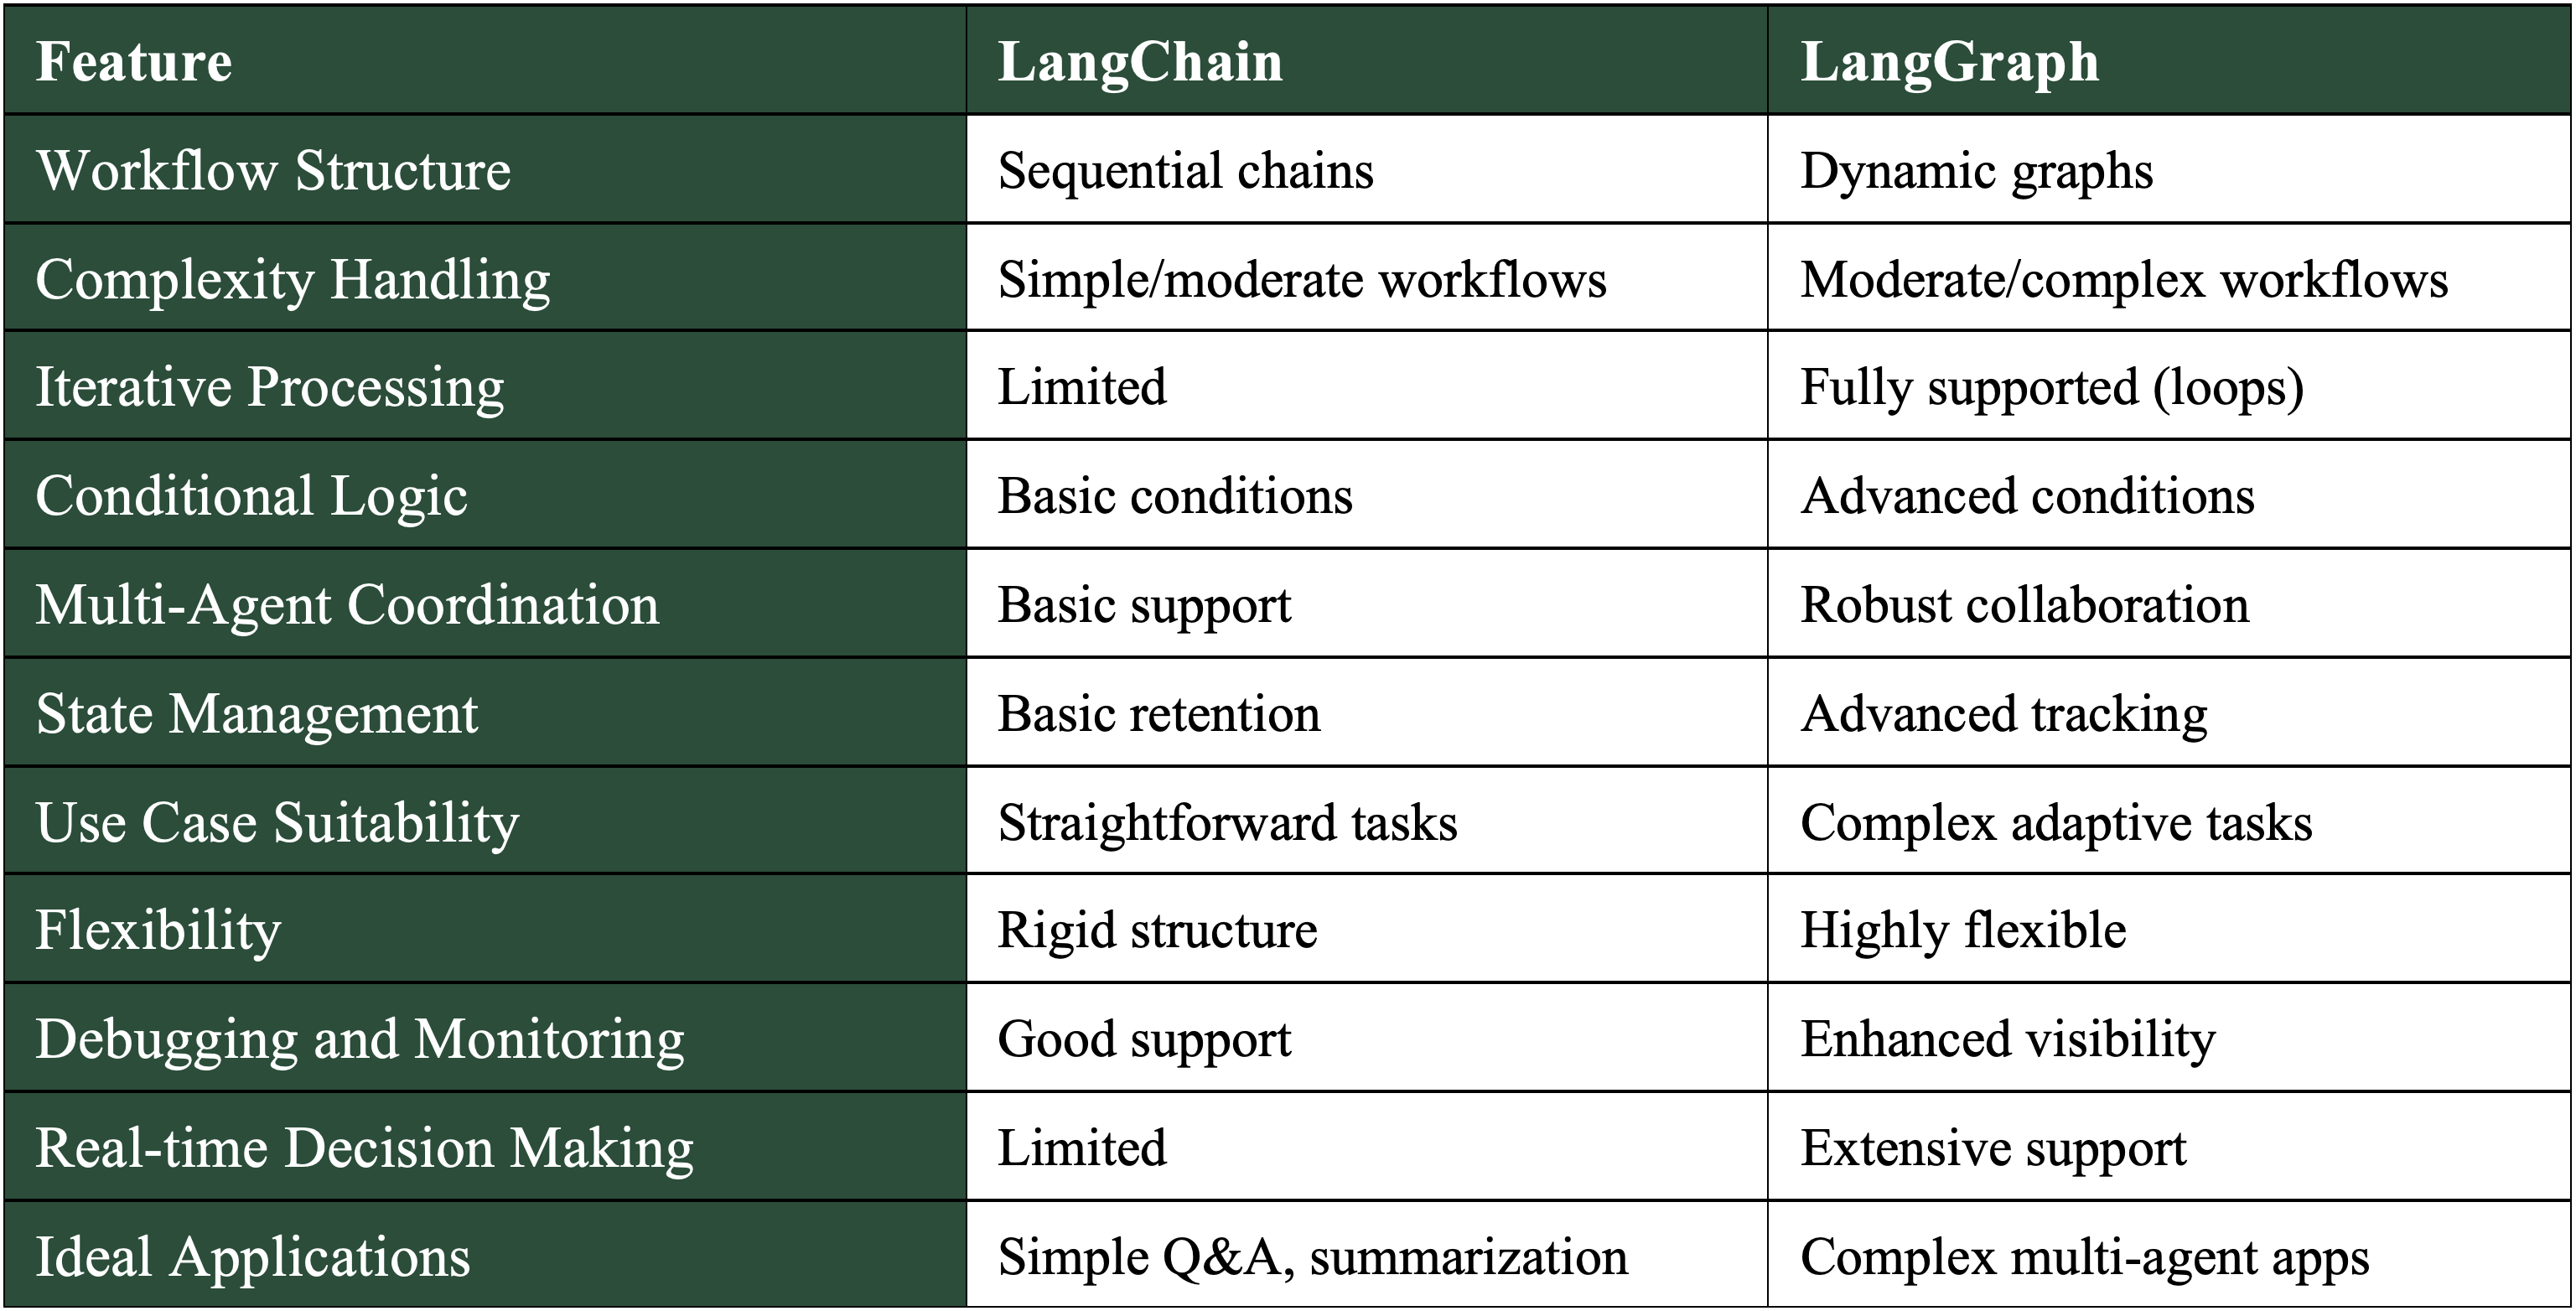
\includegraphics[width=1\textwidth]{Images/Comparison of LangChain and LangGraph.png}
    \captionof{table}{Comparison of LangChain and LangGraph}
    \label{tab:langchain_langgraph_comparison}
\end{center}

The choice between these frameworks thus depends primarily on the complexity of the intended application, where LangChain offers simplicity for linear scenarios, while LangGraph is suited for adaptive, complex applications requiring enhanced flexibility and sophisticated state management.

% Langfuse and Observability
\subsection{Langfuse and Observability}

% Overview
\subsubsection{Overview}
Langfuse is an open-source observability platform designed specifically for applications powered by Large Language Models (LLMs). It provides developers with tools to trace, debug, and analyze the behavior of LLM applications, ensuring better performance and reliability.

\begin{center}
    \centering
    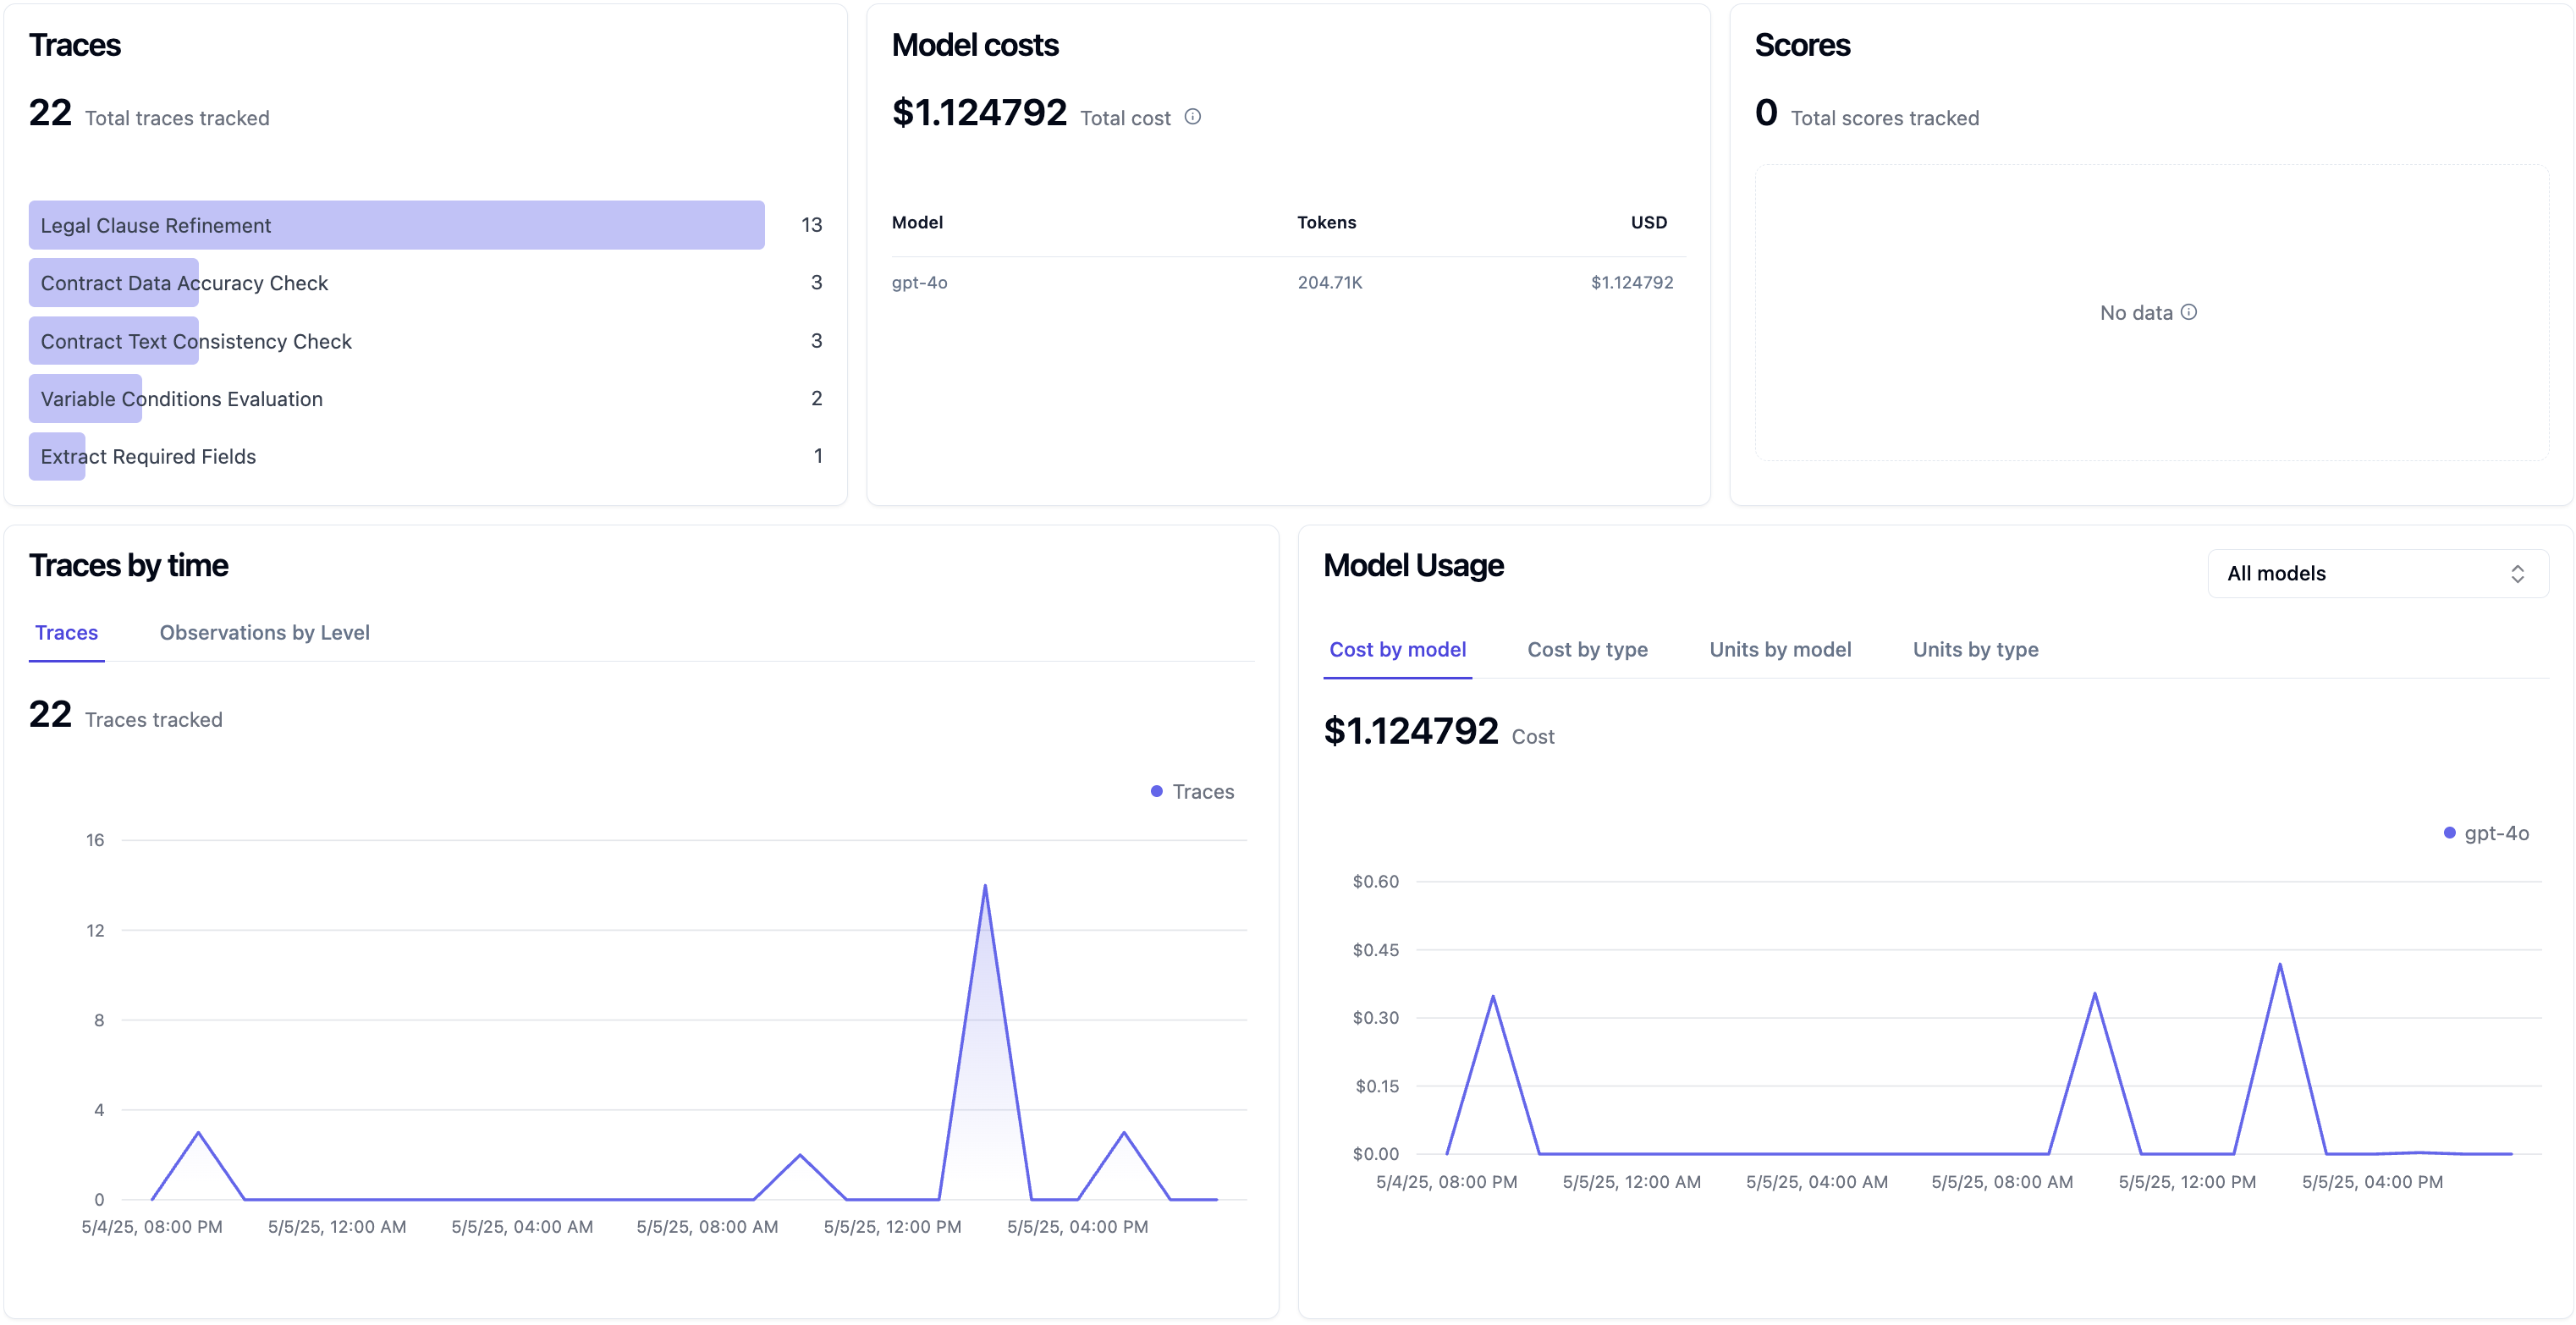
\includegraphics[width=1\textwidth]{Images/Langfuse Overview.png}
    \captionof{figure}{Langfuse Dashboard}
    \label{fig:langfuseDashboard}
\end{center}

% Key Features
\subsubsection{Key Features}
\begin{itemize}
    \item \textbf{Comprehensive Tracing}: Langfuse captures detailed traces of LLM operations, including prompts, responses, and intermediate steps, allowing developers to understand the flow of data and identify issues effectively.
    \item \textbf{Session Management}: It groups related interactions into sessions, providing a holistic view of multi-turn conversations or complex workflows.
    \item \textbf{Analytics Dashboard}: Langfuse offers dashboards that display metrics such as latency, token usage, and cost, enabling teams to monitor and optimize application performance.
    \item \textbf{Prompt Management}: The platform includes tools for managing and versioning prompts, facilitating experimentation and iterative development.
    \item \textbf{Integration Support}: Langfuse integrates seamlessly with popular frameworks like LangChain, LlamaIndex, and OpenAI SDKs, as well as supports OpenTelemetry for broader observability needs.
\end{itemize}

% Deployment Options
\subsubsection{Deployment Options}
Langfuse can be deployed in various environments:

\begin{itemize}
    \item \textbf{Cloud Hosting}: Utilize Langfuse’s managed cloud service for quick setup and scalability.
    \item \textbf{Self-Hosting}: Deploy Langfuse on-premises or in private clouds using Docker, providing full control over data and configurations.
\end{itemize}

% Use Cases
\subsubsection{Use Cases}
\begin{itemize}
    \item \textbf{Debugging Complex Workflows}: By tracing each step of LLM operations, developers can pinpoint and resolve issues in complex applications.
    \item \textbf{Performance Monitoring}: Track metrics to identify bottlenecks and optimize resource usage.
    \item \textbf{Quality Assurance}: Analyze user interactions and feedback to improve response quality and user satisfaction.
    \item \textbf{Compliance and Auditing}: Maintain detailed logs for auditing purposes, ensuring compliance with regulatory standards.
\end{itemize}

Incorporating Langfuse into the development lifecycle of LLM applications enhances transparency, reliability, and efficiency, making it an invaluable tool for teams aiming to build robust AI solutions.

% Tiptap for Rich Text Editing
\subsection{Tiptap for Rich Text Editing}

% Overview
\subsubsection{Overview}
Tiptap is a headless, open-source rich text editor framework built on ProseMirror, designed for developers seeking full control over their content editing interfaces. Its modular architecture and extensive extension ecosystem make it a powerful tool for building customized, collaborative, and AI-enhanced editing experiences.

\begin{center}
    \centering
    
\includegraphics[width=0.8\textwidth]{Images/Tiptap editor.jpg}
    \captionof{figure}{Tiptap Editor} \cite{tiptap_editor}
    \label{fig:tiptap_editor}
\end{center}

% Architecture and Core Concepts
\subsubsection{Architecture and Core Concepts}
Tiptap is a headless, framework-agnostic rich text editor built on top of ProseMirror, designed to provide developers with full control over the editor’s functionality and appearance. Its architecture is modular and extensible, allowing for the creation of customized editing experiences.

\begin{center}
    \centering
    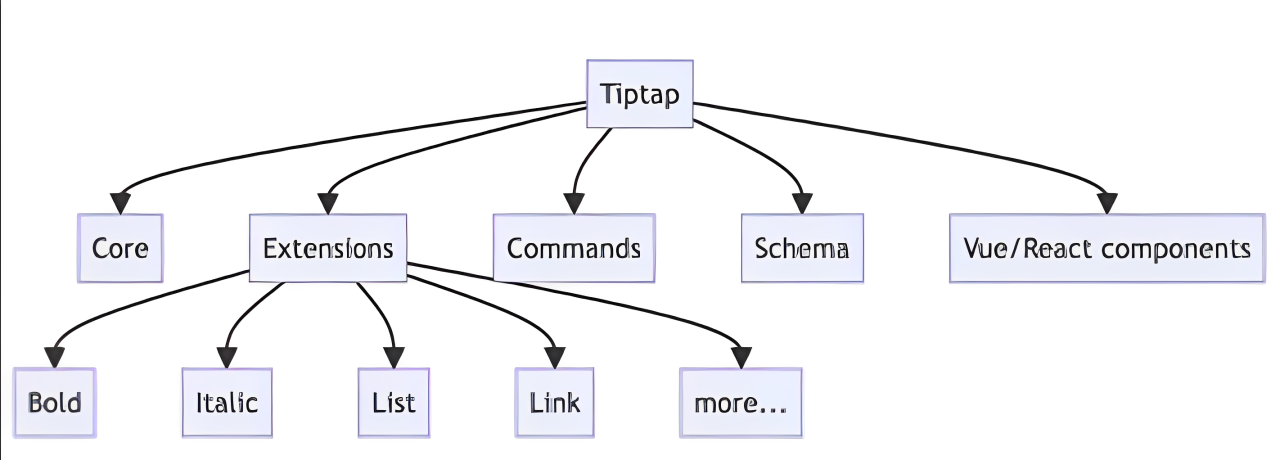
\includegraphics[width=0.8\textwidth]{Images/Tiptap Architecture.png}
    \captionof{figure}{Tiptap Architecture}
    \label{fig:tiptapArchitecture}
\end{center}

Key Architectural Components:
\begin{itemize}
    \item \textbf{Schema}: Defines the structure of the document, specifying the allowed nodes (e.g., paragraphs, headings) and marks (e.g., bold, italic). This strict schema ensures content consistency and predictability.
    \item \textbf{State}: Represents the current content and selection within the editor. It is immutable and updated through transactions, enabling features like undo/redo and collaborative editing.
    \item \textbf{Transaction}: Encapsulates changes to the state, such as text insertions or formatting. Transactions ensure that state changes are predictable and manageable.
    \item \textbf{Extensions}: Modular units that add functionality to the editor, such as new nodes, marks, commands, or plugins. Tiptap provides a rich set of core and community extensions, and developers can create custom ones as needed.
    \item \textbf{Commands}: Functions that perform actions within the editor, often used to manipulate the document or respond to user input. Commands can be chained for complex operations.
\end{itemize}

% Key Features
\subsubsection{Key Features}
\begin{itemize}
    \item \textbf{Extension-Based Modularity}: Tiptap offers over 100 extensions, including both open-source and Pro options, allowing developers to tailor the editor’s functionality to specific needs.
    \item \textbf{Real-Time Collaboration}: Through integrations like Hocuspocus and CRDTs, Tiptap supports collaborative editing with features like live cursors and offline synchronization.
    \item \textbf{AI Integration}: The Content AI extension enables in-editor AI capabilities such as text suggestions, translations, and content generation, enhancing the writing experience.
    \item \textbf{Framework Agnostic}: Tiptap’s design allows it to be integrated into various JavaScript frameworks, providing flexibility in application development.
\end{itemize}

% Use Cases
\subsubsection{Use Cases}
Tiptap is suitable for a wide range of applications, including:
\begin{itemize}
    \item Building Notion-like editors with custom blocks and interactions.
    \item Developing collaborative document editing platforms.
    \item Creating AI-assisted writing tools with real-time suggestions.
    \item Implementing rich text editors in CMS platforms. 
\end{itemize}    

Tiptap stands out as a versatile and developer-friendly rich text editor framework. Its combination of headless architecture, modular extensions, and support for real-time collaboration and AI integration makes it a compelling choice for modern web applications requiring customized content editing solutions.

% Project Requirements
\section{Specification of Requirements}
Given the agile nature of the project, the actors as well as functional and non-functional requirements are subject to evolve. The elements below reflect the current state of the project.

% Business Architecture
\subsection{Business Architecture}
The business architecture depicted in Figure~\ref{fig:business_architecture} outlines the overarching structure and planned components of the intelligent contract management platform. The platform integrates three main components supported by robust underlying layers of data management, security, observability, and tool integration capabilities.

\begin{center}
    \centering
    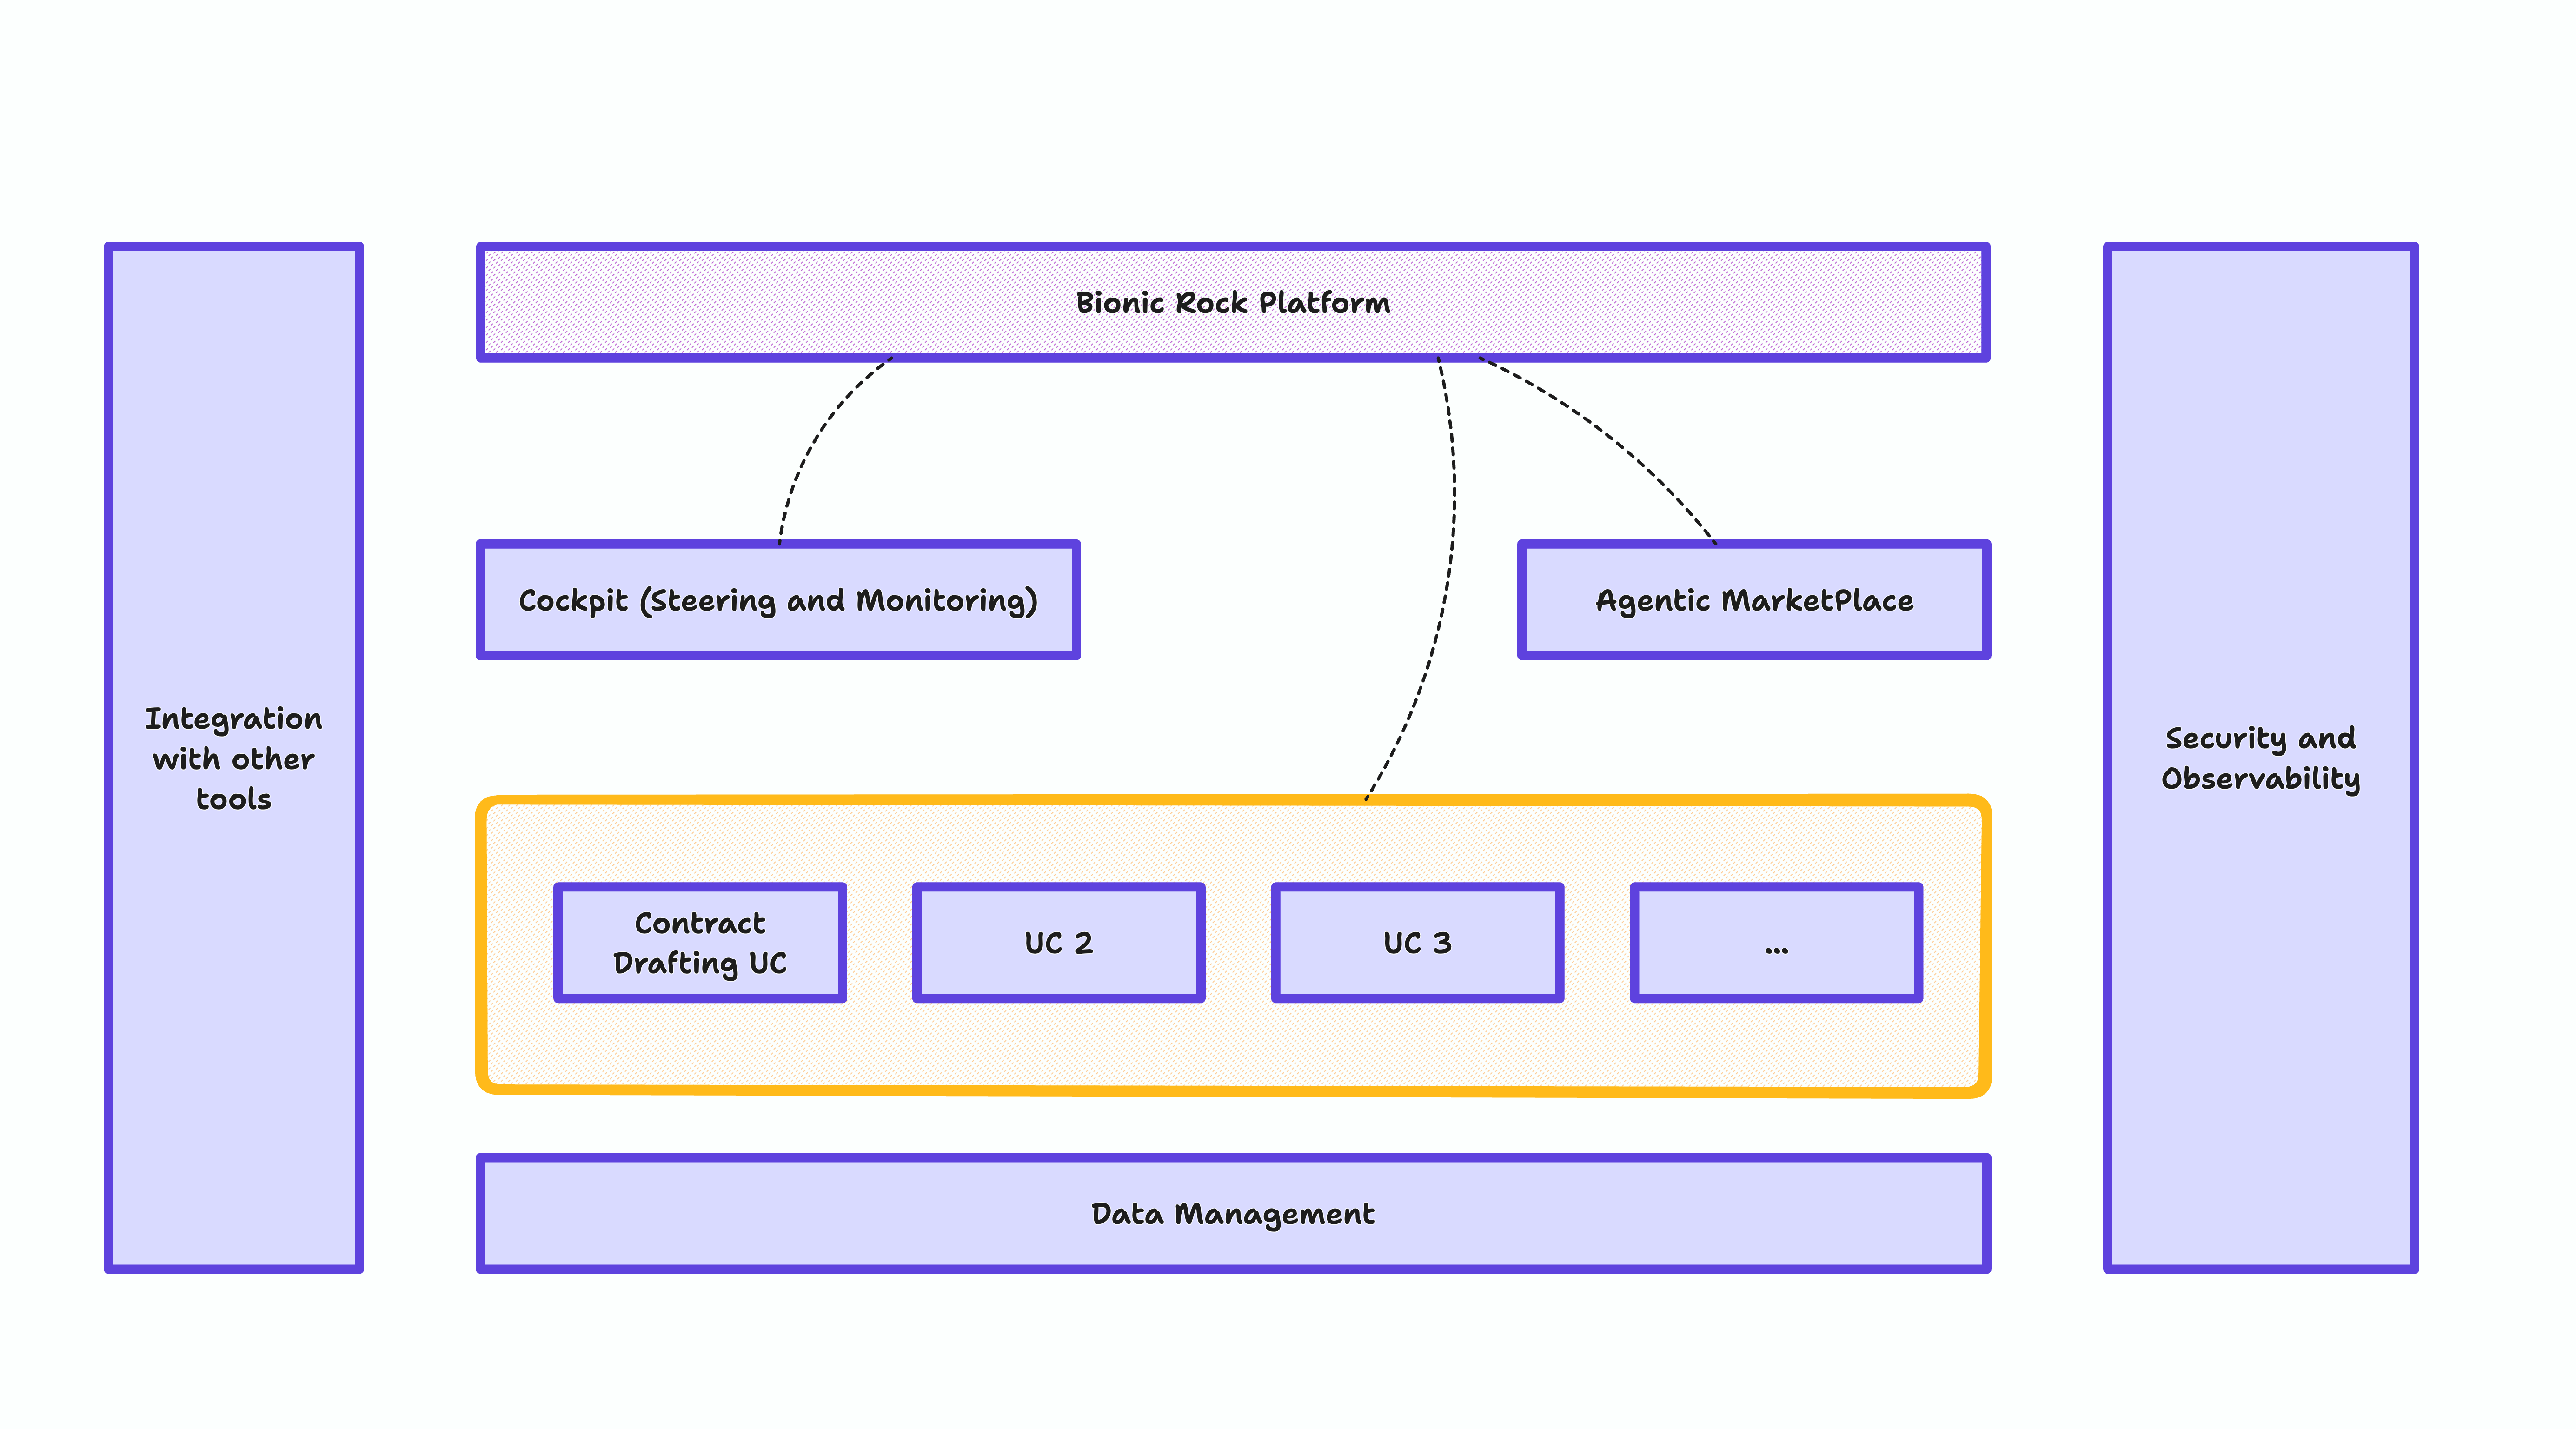
\includegraphics[width=0.9\textwidth]{Images/Business Architecture.png}
    \captionof{figure}{Business Architecture Overview}
    \label{fig:business_architecture}
\end{center}

The platform structure is organized into three core areas:

\begin{itemize}
\item \textbf{Cockpit (Steering and Monitoring)}: This area provides oversight and real-time analytics, enabling stakeholders to monitor system performance, track usage, and manage workflows effectively.
\item \textbf{Agentic Marketplace}: Designed to host various autonomous AI agents, this component facilitates the scalable deployment and orchestration of intelligent services, supporting diverse, dynamic business needs and agent interactions.
\item \textbf{Use Case Features}: These represent modular functionalities tailored to specific business processes. The primary use case currently prioritized is the \textbf{Contract Drafting Use Case (UC)}, scheduled for completion within a 21-week timeframe. This use case is central to my internship project and focuses on automating and enhancing the contract drafting process through intelligent clause selection, AI-assisted drafting, compliance verification, and collaboration enhancements.
\end{itemize}

These foundational components are encapsulated within a broader environment of:

\begin{itemize}
\item \textbf{Data Management}: Ensures consistent data governance, quality, and efficient access to support the platform's intelligent features.
\item \textbf{Integration with Other Tools}: Provides seamless interoperability with external and internal enterprise applications, extending the platform's capabilities and ensuring a cohesive user experience.
\item \textbf{Security and Observability}: Delivers comprehensive security measures and observability tools to protect data integrity, ensure compliance, and provide transparent system monitoring and diagnostics.
\end{itemize}

This structured business architecture aims to offer a scalable, secure, and integrative platform capable of addressing complex legal operations through advanced technological solutions.

% Actor Identification
\subsection{Actor Identification}
An actor specifies a role played by a user or any other system interacting with the solution. Actors are always external to the system, interacting by initiating a use case, providing inputs, or receiving outputs. In the context of our platform, we have two types of actors:

\begin{center}
    \centering
    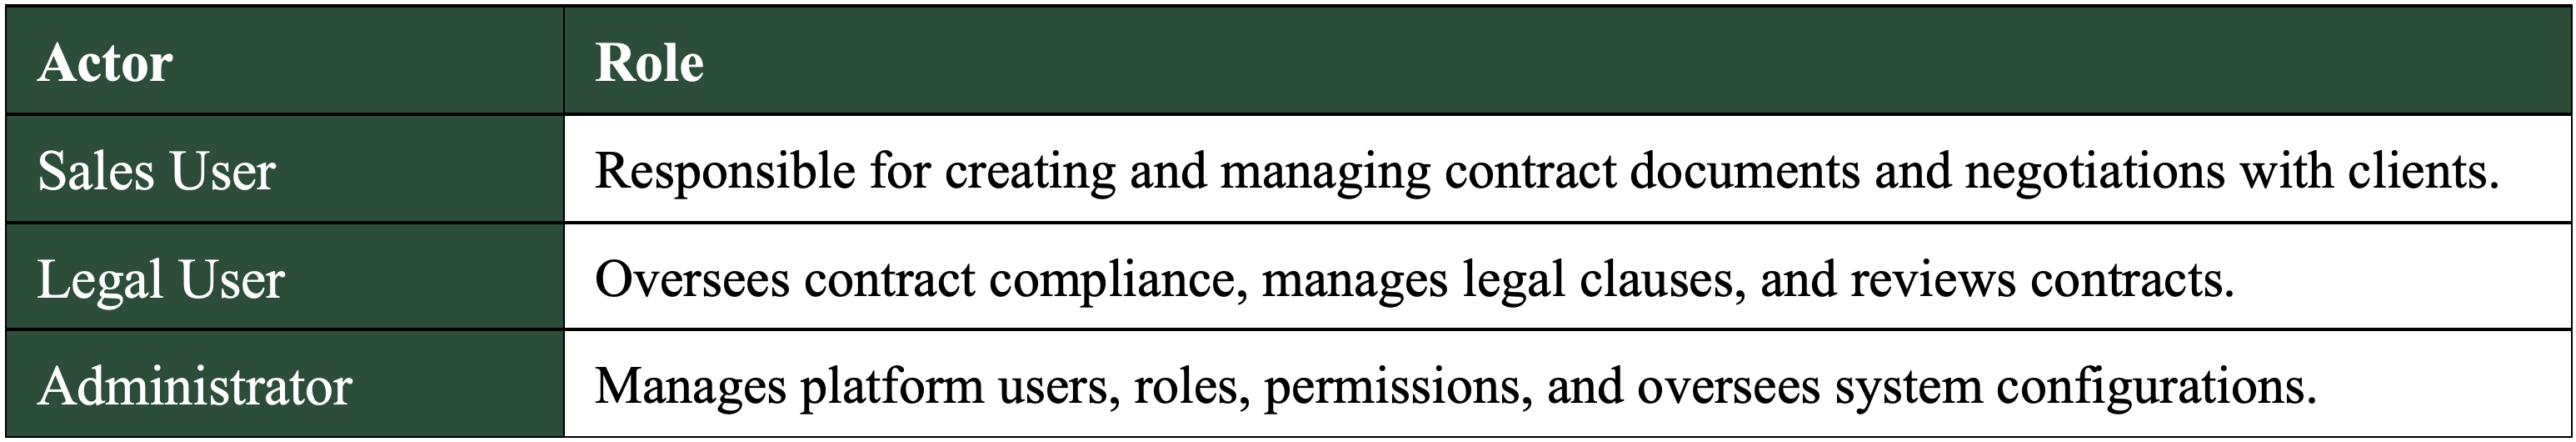
\includegraphics[width=1\textwidth]{Images/Actors and Their Roles.png}
    \captionof{table}{Actors and Their Roles}
    \label{tab:actors_and_roles}
\end{center}

% Functional Requirements
\subsection{Functional Requirements}

% Authentication
\subsubsection{Authentication}
The application must enable users to authenticate using a username or email and password.

% Sales User Functionalities
\subsubsection{Sales User Functionalities}

\textbf{Contract Generation}:\vspace{0.4em}
\begin{adjustwidth}{3em}{1em}
    \begin{itemize}
        \item The sales user must be able to create a new contract.\vspace{0.4em}
        \item The sales user must be able to create a new client.
    \end{itemize}
\end{adjustwidth}\vspace{0.85em}

\textbf{Contract Editing}:\vspace{0.4em}
\begin{adjustwidth}{3em}{1em}
    \begin{itemize}
        \item The Sales user must be able to access the rich-text contract editor.\vspace{0.4em}
        \item The Sales user must be able to create clause requests.\vspace{0.4em}
        \item The Sales user must be able to modify contract variables.\vspace{0.4em}
        \item The Sales user must be able to track changes across different contract versions.  
    \end{itemize}
\end{adjustwidth}\vspace{0.85em} 

\textbf{Contract Review \& Compliance}:\vspace{0.4em}
\begin{adjustwidth}{3em}{1em}
    \begin{itemize}
        \item The Sales user must be able to trigger AI-powered compliance checks.\vspace{0.4em}
        \item The Sales user must be able to change the contract status (e.g., in editing, in review, finalized).
    \end{itemize}
\end{adjustwidth}\vspace{0.85em} 

\textbf{Export, Sharing, and Management}:\vspace{0.4em}
\begin{adjustwidth}{3em}{1em}
    \begin{itemize}
        \item The Sales user must be able to access only the contracts they have created.\vspace{0.4em}
        \item The Sales user must be able to export contracts as downloadable files (Word, PDF).\vspace{0.4em}
        \item The Sales user must be able to share contracts via secure links or email attachments.\vspace{0.4em}
        \item The Sales user must be able to archive and delete contracts.
    \end{itemize}
\end{adjustwidth}\vspace{0.85em}  

% Legal User Functionalities
\subsubsection{Legal User Functionalities}

\textbf{Clause Management}:\vspace{0.4em}
\begin{adjustwidth}{3em}{1em}
    \begin{itemize}
        \item The Legal user must be able to review clause requests from Sales.\vspace{0.4em}
        \item The Legal user must be able to refine clause content using AI assistance.\vspace{0.4em}
        \item The Legal user must be able to create, insert, modify, and delete legal clauses.  
    \end{itemize}
\end{adjustwidth}\vspace{0.85em} 

\textbf{Contract Editing and Versioning}:\vspace{0.4em}
\begin{adjustwidth}{3em}{1em}
    \begin{itemize}
        \item The Legal user must be able to access and create versions of contracts.\vspace{0.4em}
        \item The Legal user must be able to restore previous contract versions.\vspace{0.4em}
        \item The Legal user must be able to edit contracts using a rich-text editor.\vspace{0.4em}
        \item The Legal user must be able to modify contract variables.
    \end{itemize}
\end{adjustwidth}\vspace{0.85em} 

\textbf{Contract Review \& Compliance}:\vspace{0.4em}
\begin{adjustwidth}{3em}{1em}
    \begin{itemize}
        \item The Legal user must be able to trigger AI-powered compliance checks.\vspace{0.4em}
        \item The Legal user must be able to change the status of a contract (e.g., in editing, in review).
    \end{itemize}
\end{adjustwidth}\vspace{0.85em} 

\textbf{Export, Sharing, and Management}:\vspace{0.4em}
\begin{adjustwidth}{3em}{1em}
    \begin{itemize}
        \item The Legal user must be able to access all existing contracts.\vspace{0.4em}
        \item The Legal user must be able to export contracts as downloadable files (Word, PDF).\vspace{0.4em}
        \item The Legal user must be able to share contracts via secure links or email attachments.
    \end{itemize}
\end{adjustwidth}\vspace{0.85em} 

% Administrator Functionalities
\subsubsection{Administrator Functionalities}

\textbf{User Management}:\vspace{0.4em}
\begin{adjustwidth}{3em}{1em}
    \begin{itemize}
        \item The administrator must be able to add, modify, or remove platform users.\vspace{0.4em}
        \item The administrator must be able to manage role-based access permissions.
    \end{itemize}
\end{adjustwidth}\vspace{0.85em} 

\textbf{System Configuration}:\vspace{0.4em}
\begin{adjustwidth}{3em}{1em}
    \begin{itemize}
        \item The administrator must be able to configure integration settings and security parameters.\vspace{0.4em}
        \item The administrator must be able to monitor system performance through administrative dashboards.
    \end{itemize}
\end{adjustwidth}\vspace{0.85em} 

% Non-Functional Requirements
\subsection{Non-Functional Requirements}
\begin{itemize}
    \item \textbf{Usability}: High intuitiveness and ease of use for Sales, Legal, and Admin users, promoting efficient adoption across roles.
    \item \textbf{Maintainability}: Modular and well-documented architecture to facilitate smooth updates, debugging, and feature evolution.
    \item \textbf{Security}: Robust access control, secure data handling, and full compliance with applicable legal and organizational standards.
    \item \textbf{System Responsiveness}: Fast UI response, low-latency AI processing, and efficient data retrieval for optimal user experience.
    \item \textbf{Scalability}: Capacity to handle increased user load and data volume while maintaining system performance.
\end{itemize}

% Use Case Diagram
\subsection{Use Case Diagram}
The Use Case Diagram presented in Figure~\ref{fig:use_case_diagram} visually represents the interactions between the identified actors—Sales Users, Legal Users, and Administrators—and the main functionalities offered by the intelligent contract management platform. It illustrates how each user group engages with distinct and shared system features, clearly depicting the overall workflow from contract drafting and editing to compliance verification, version control, and collaboration activities.

\begin{center}
    \centering
    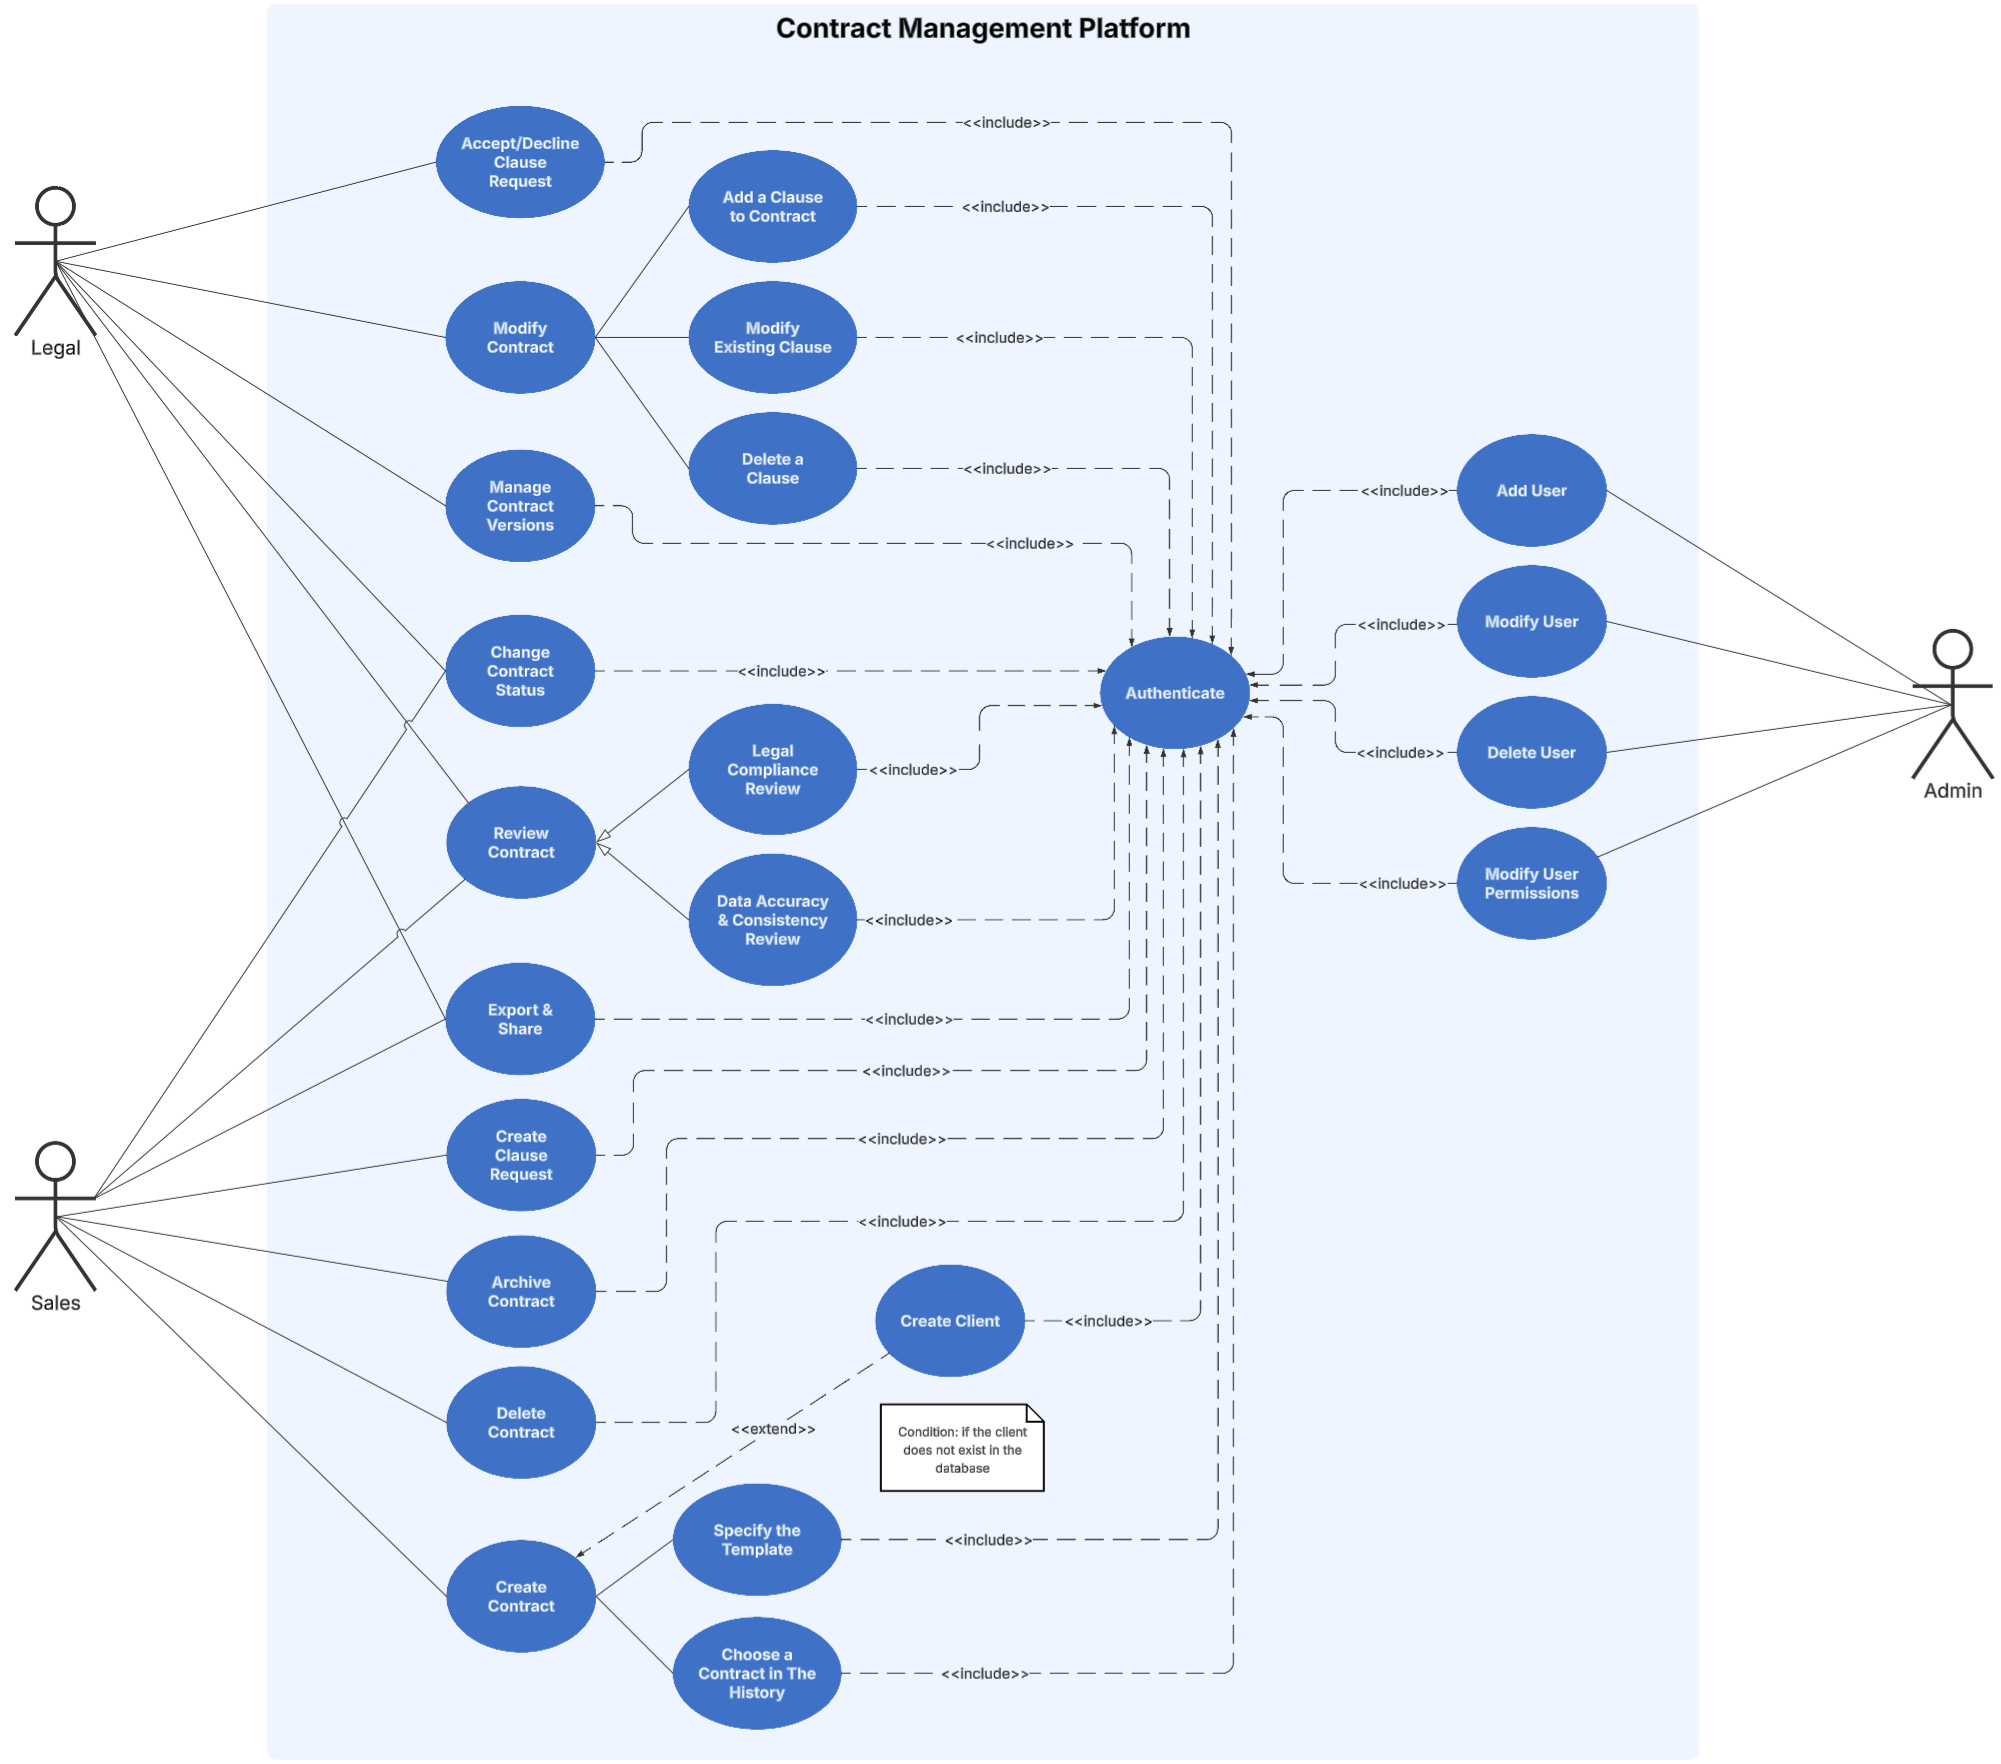
\includegraphics[width=1\textwidth]{Images/Use Case Diagram.png}
    \captionof{figure}{Use Case Diagram}
    \label{fig:use_case_diagram}
\end{center}

% Textual Description
\subsection{Textual Description}

To describe the dynamics of a use case, it is essential to enumerate all interactions between the actor and the system in textual form. This description is crucial, as it facilitates clear communication with all stakeholders and ensures a shared understanding of the business terminology involved.

\textbf{Textual Description of Use Case: Create Contract}\vspace{-0.3cm}

\begin{center}
    \centering
    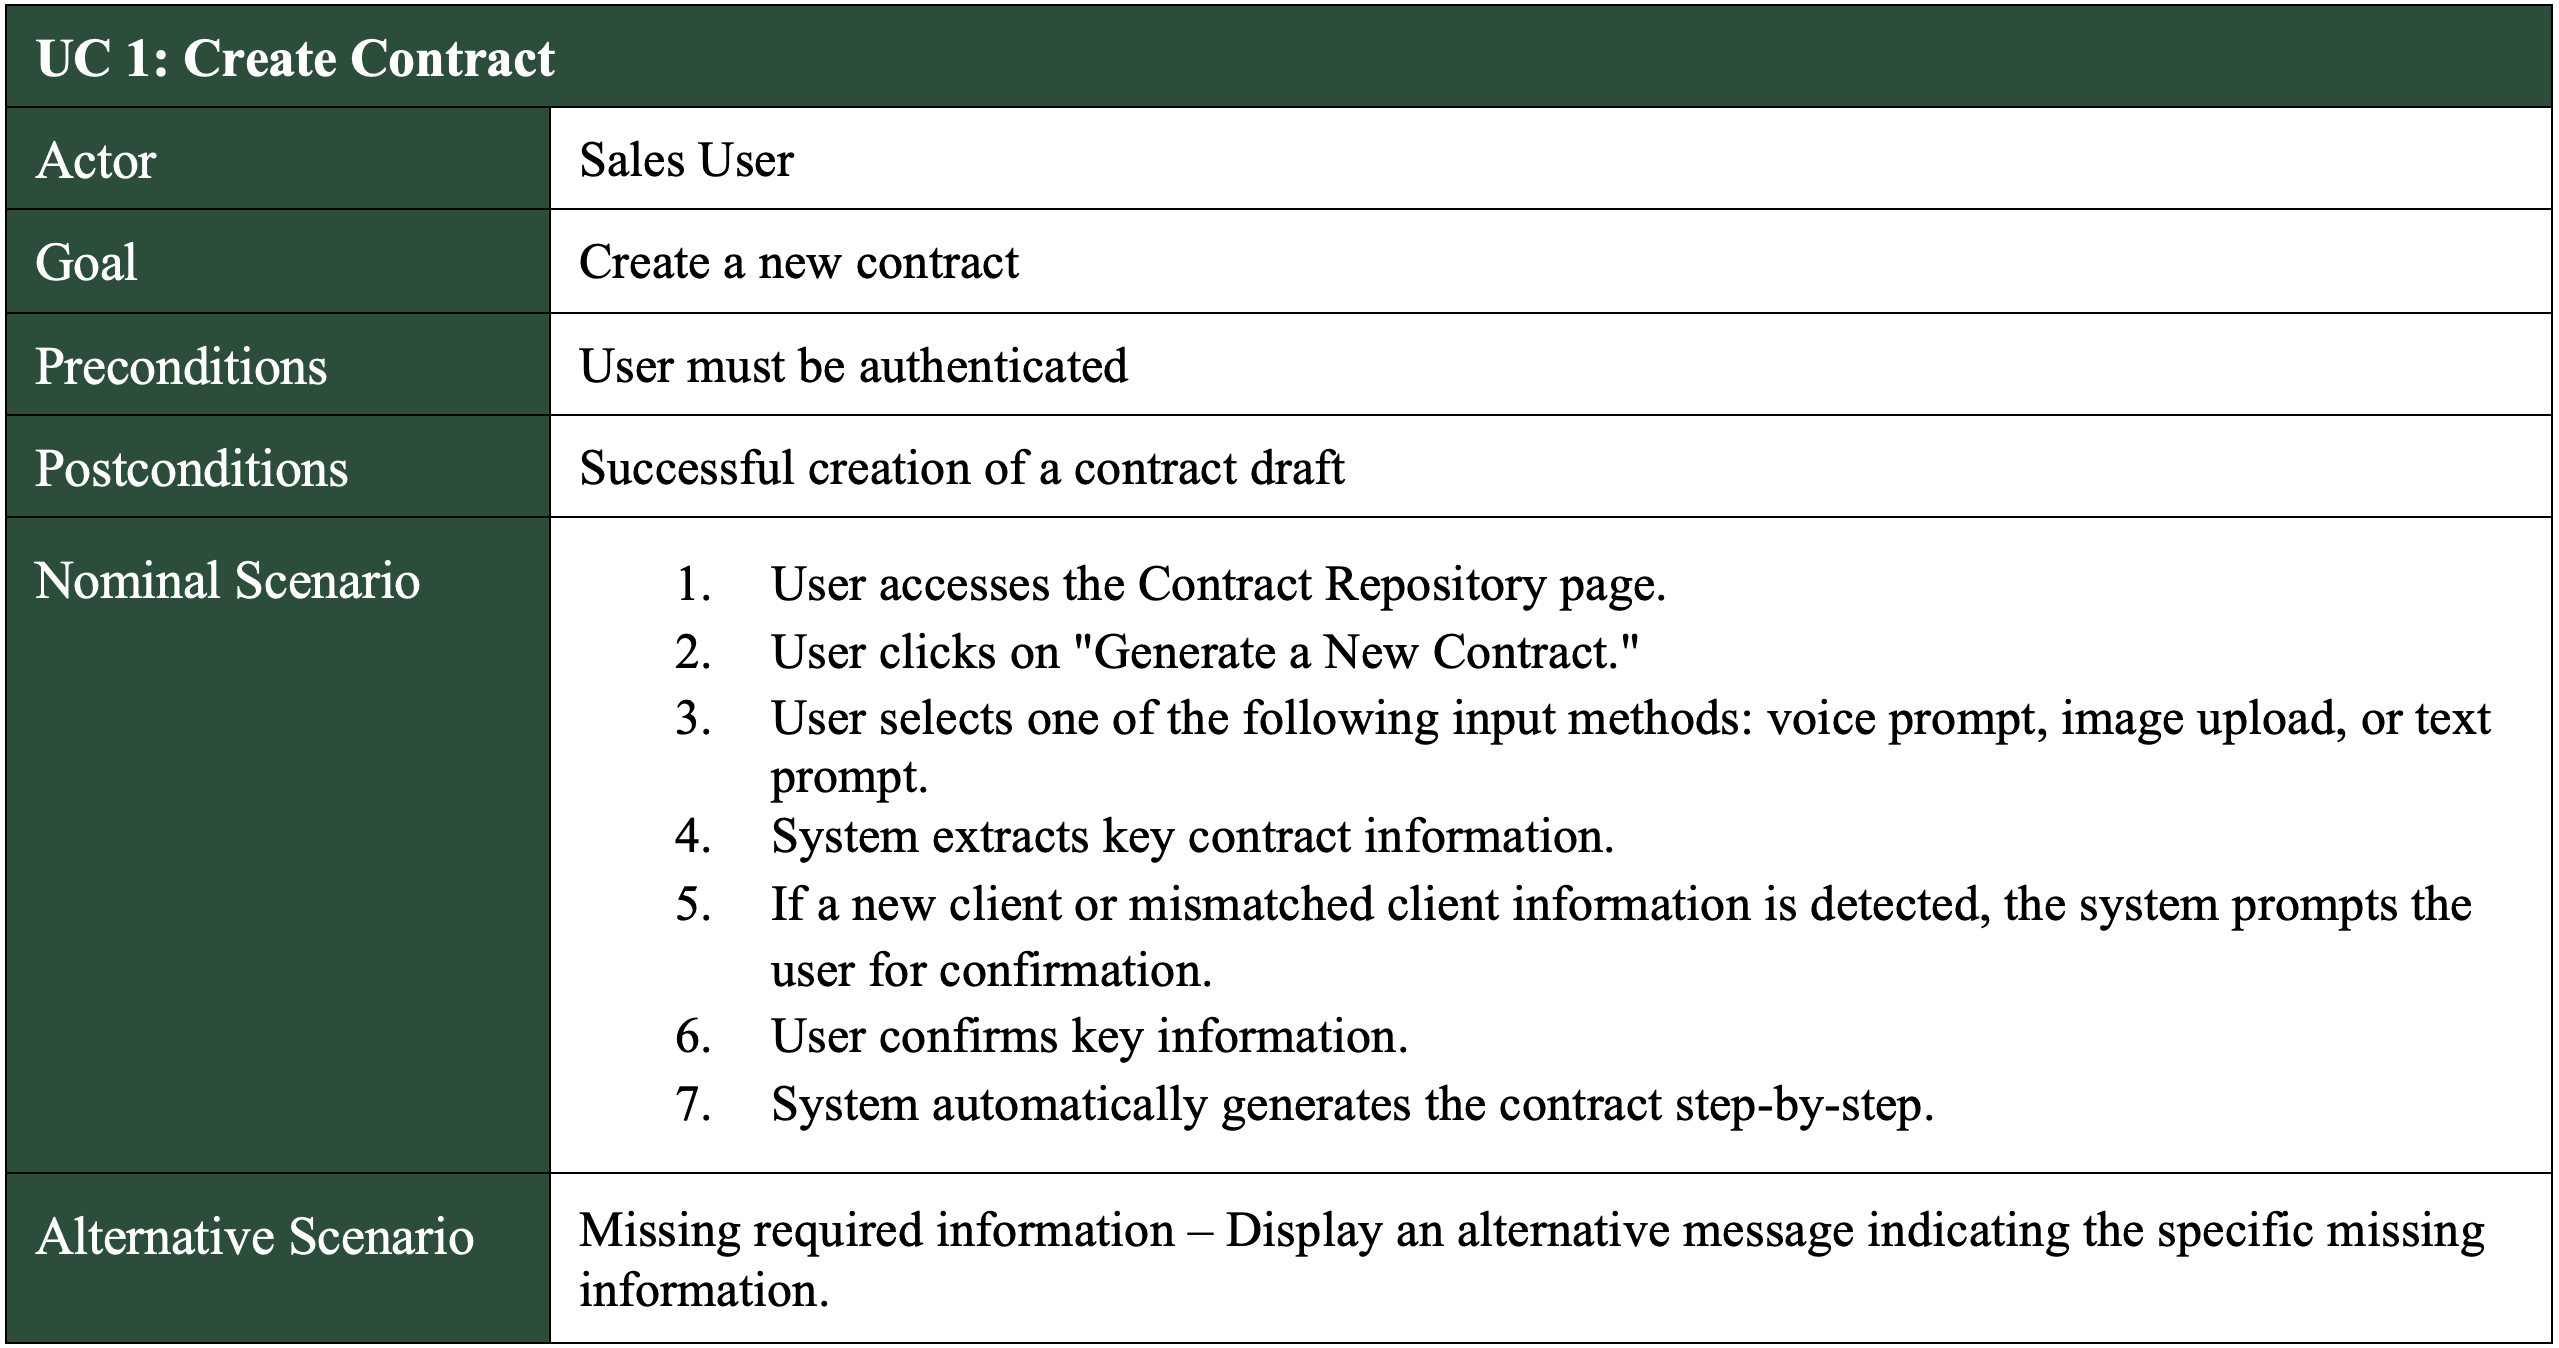
\includegraphics[width=1\textwidth]{Images/Create Contract Use Case.png}
    \captionof{table}{Textual Description of Use Case: Create Contract}
    \label{tab:create_contract_use_case}
\end{center}

\vspace{0.3cm}

\textbf{Textual Description of Use Case: Create Clause Request}\vspace{-0.3cm}

\begin{center}
    \centering
    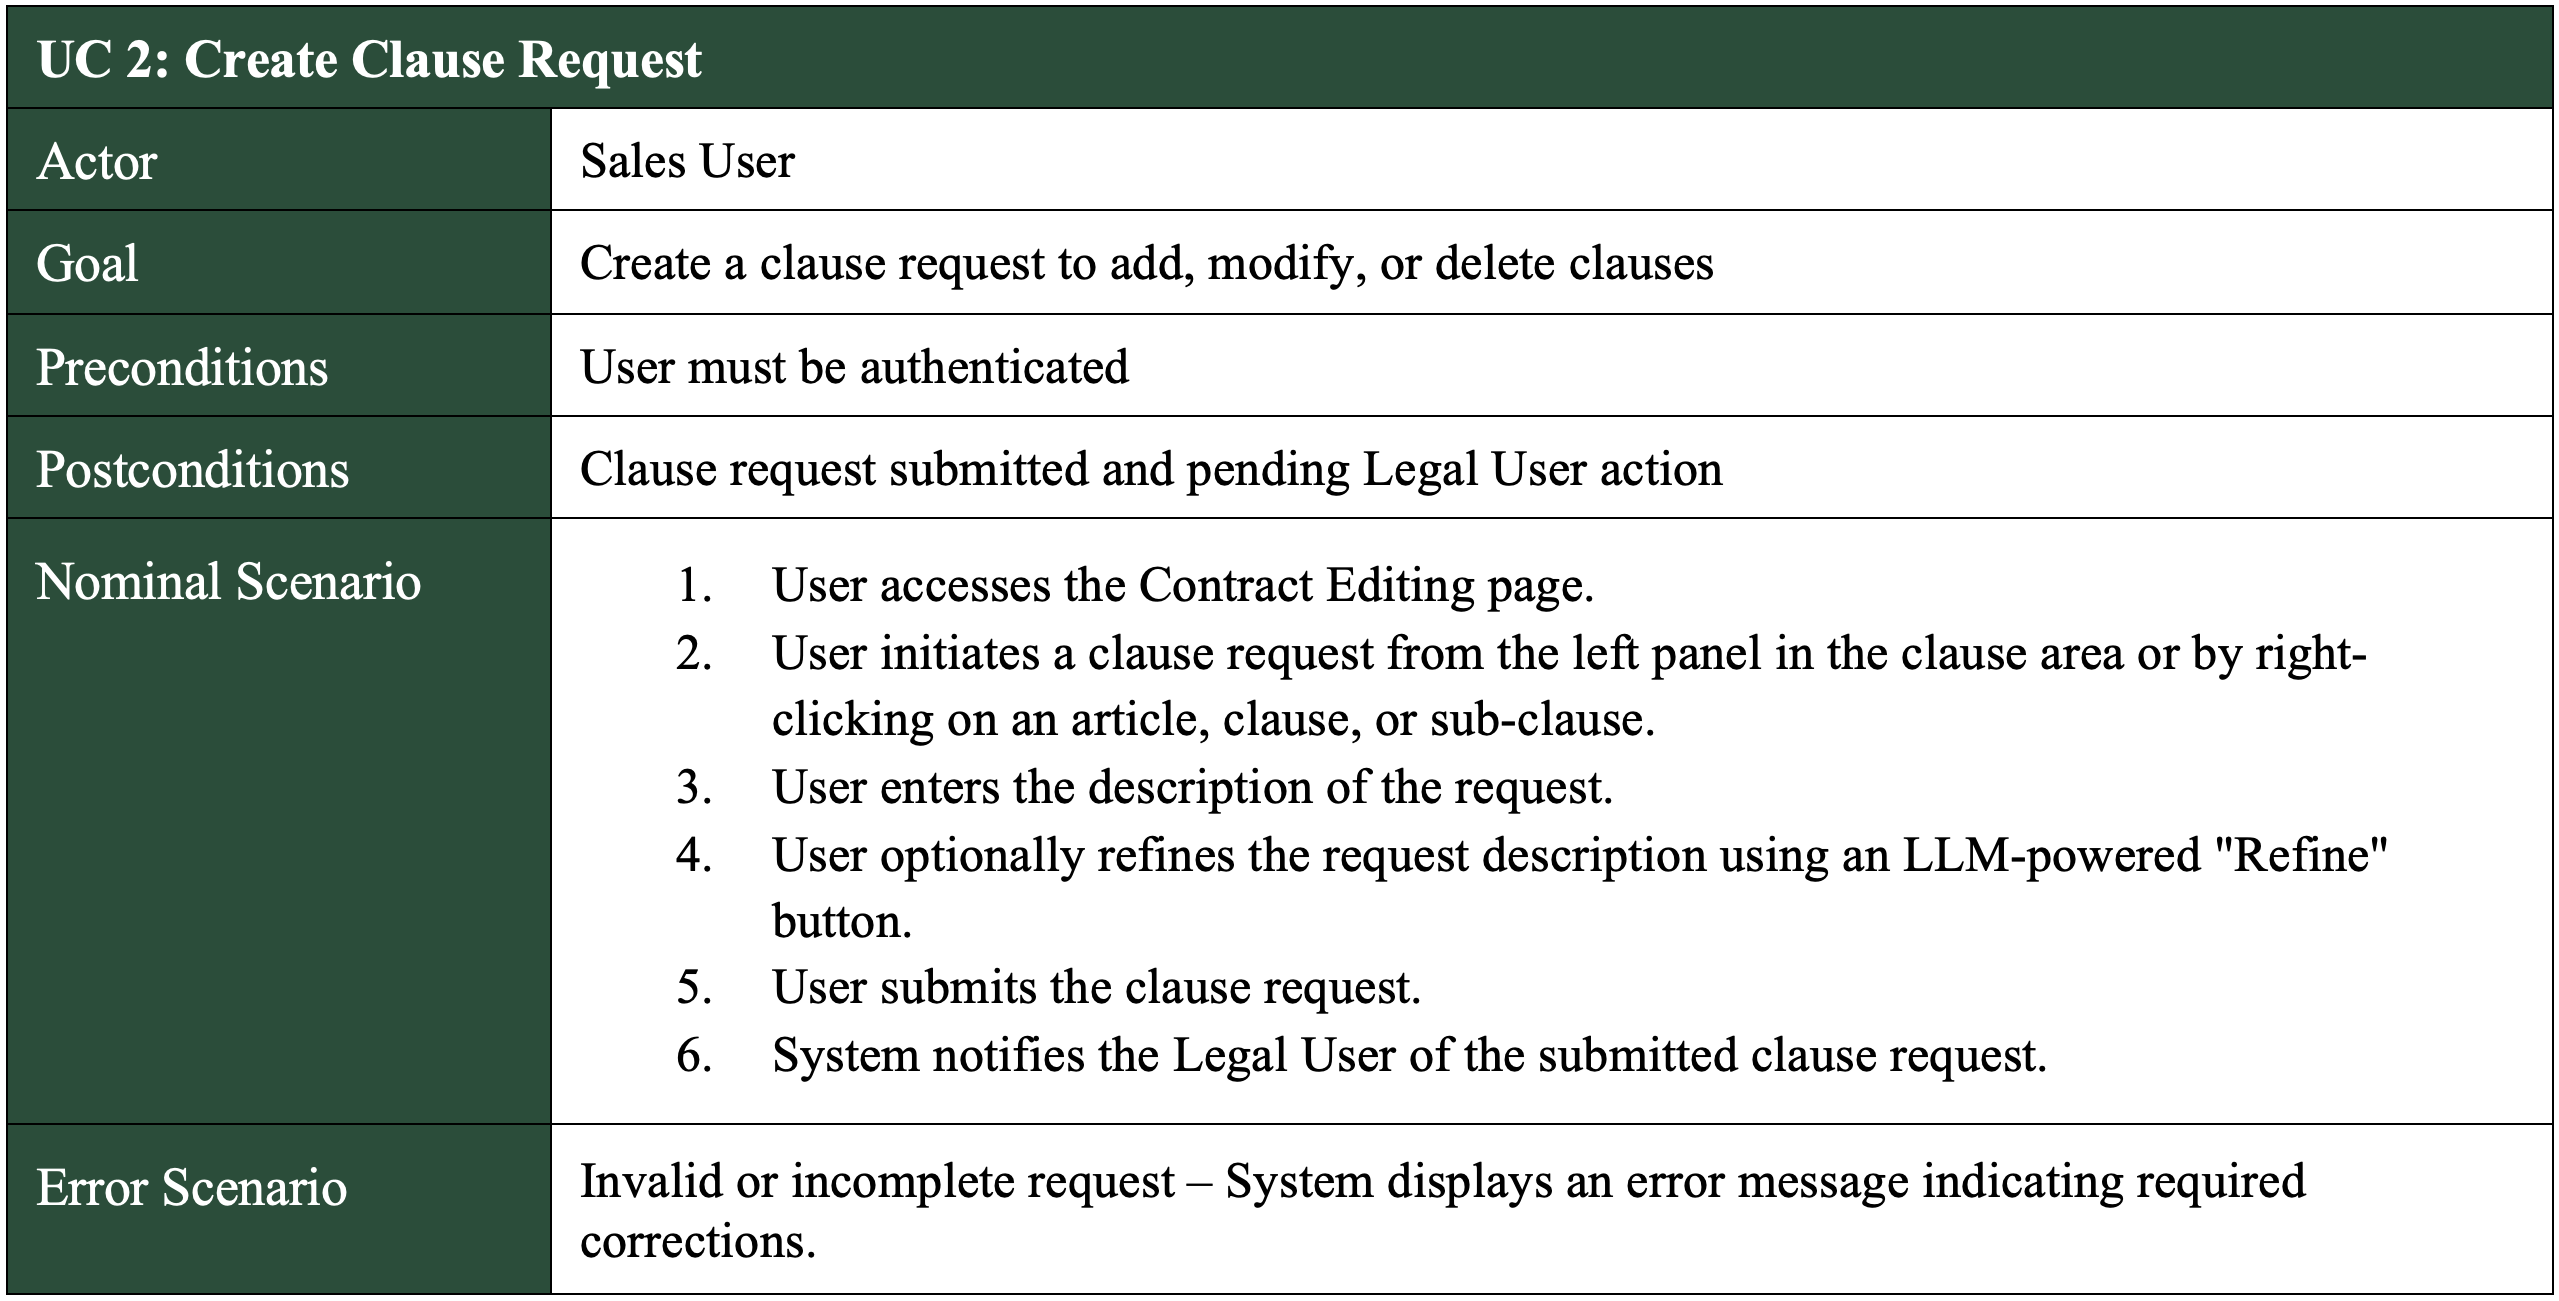
\includegraphics[width=1\textwidth]{Images/Create Clause Request Use Case.png}
    \captionof{table}{Textual Description of Use Case: Create Clause Request}
    \label{tab:create_clause_request_use_case}
\end{center}

\vspace{0.3cm}

\textbf{Textual Description of Use Case: Review Contract}\vspace{-0.3cm}

\begin{center}
    \centering
    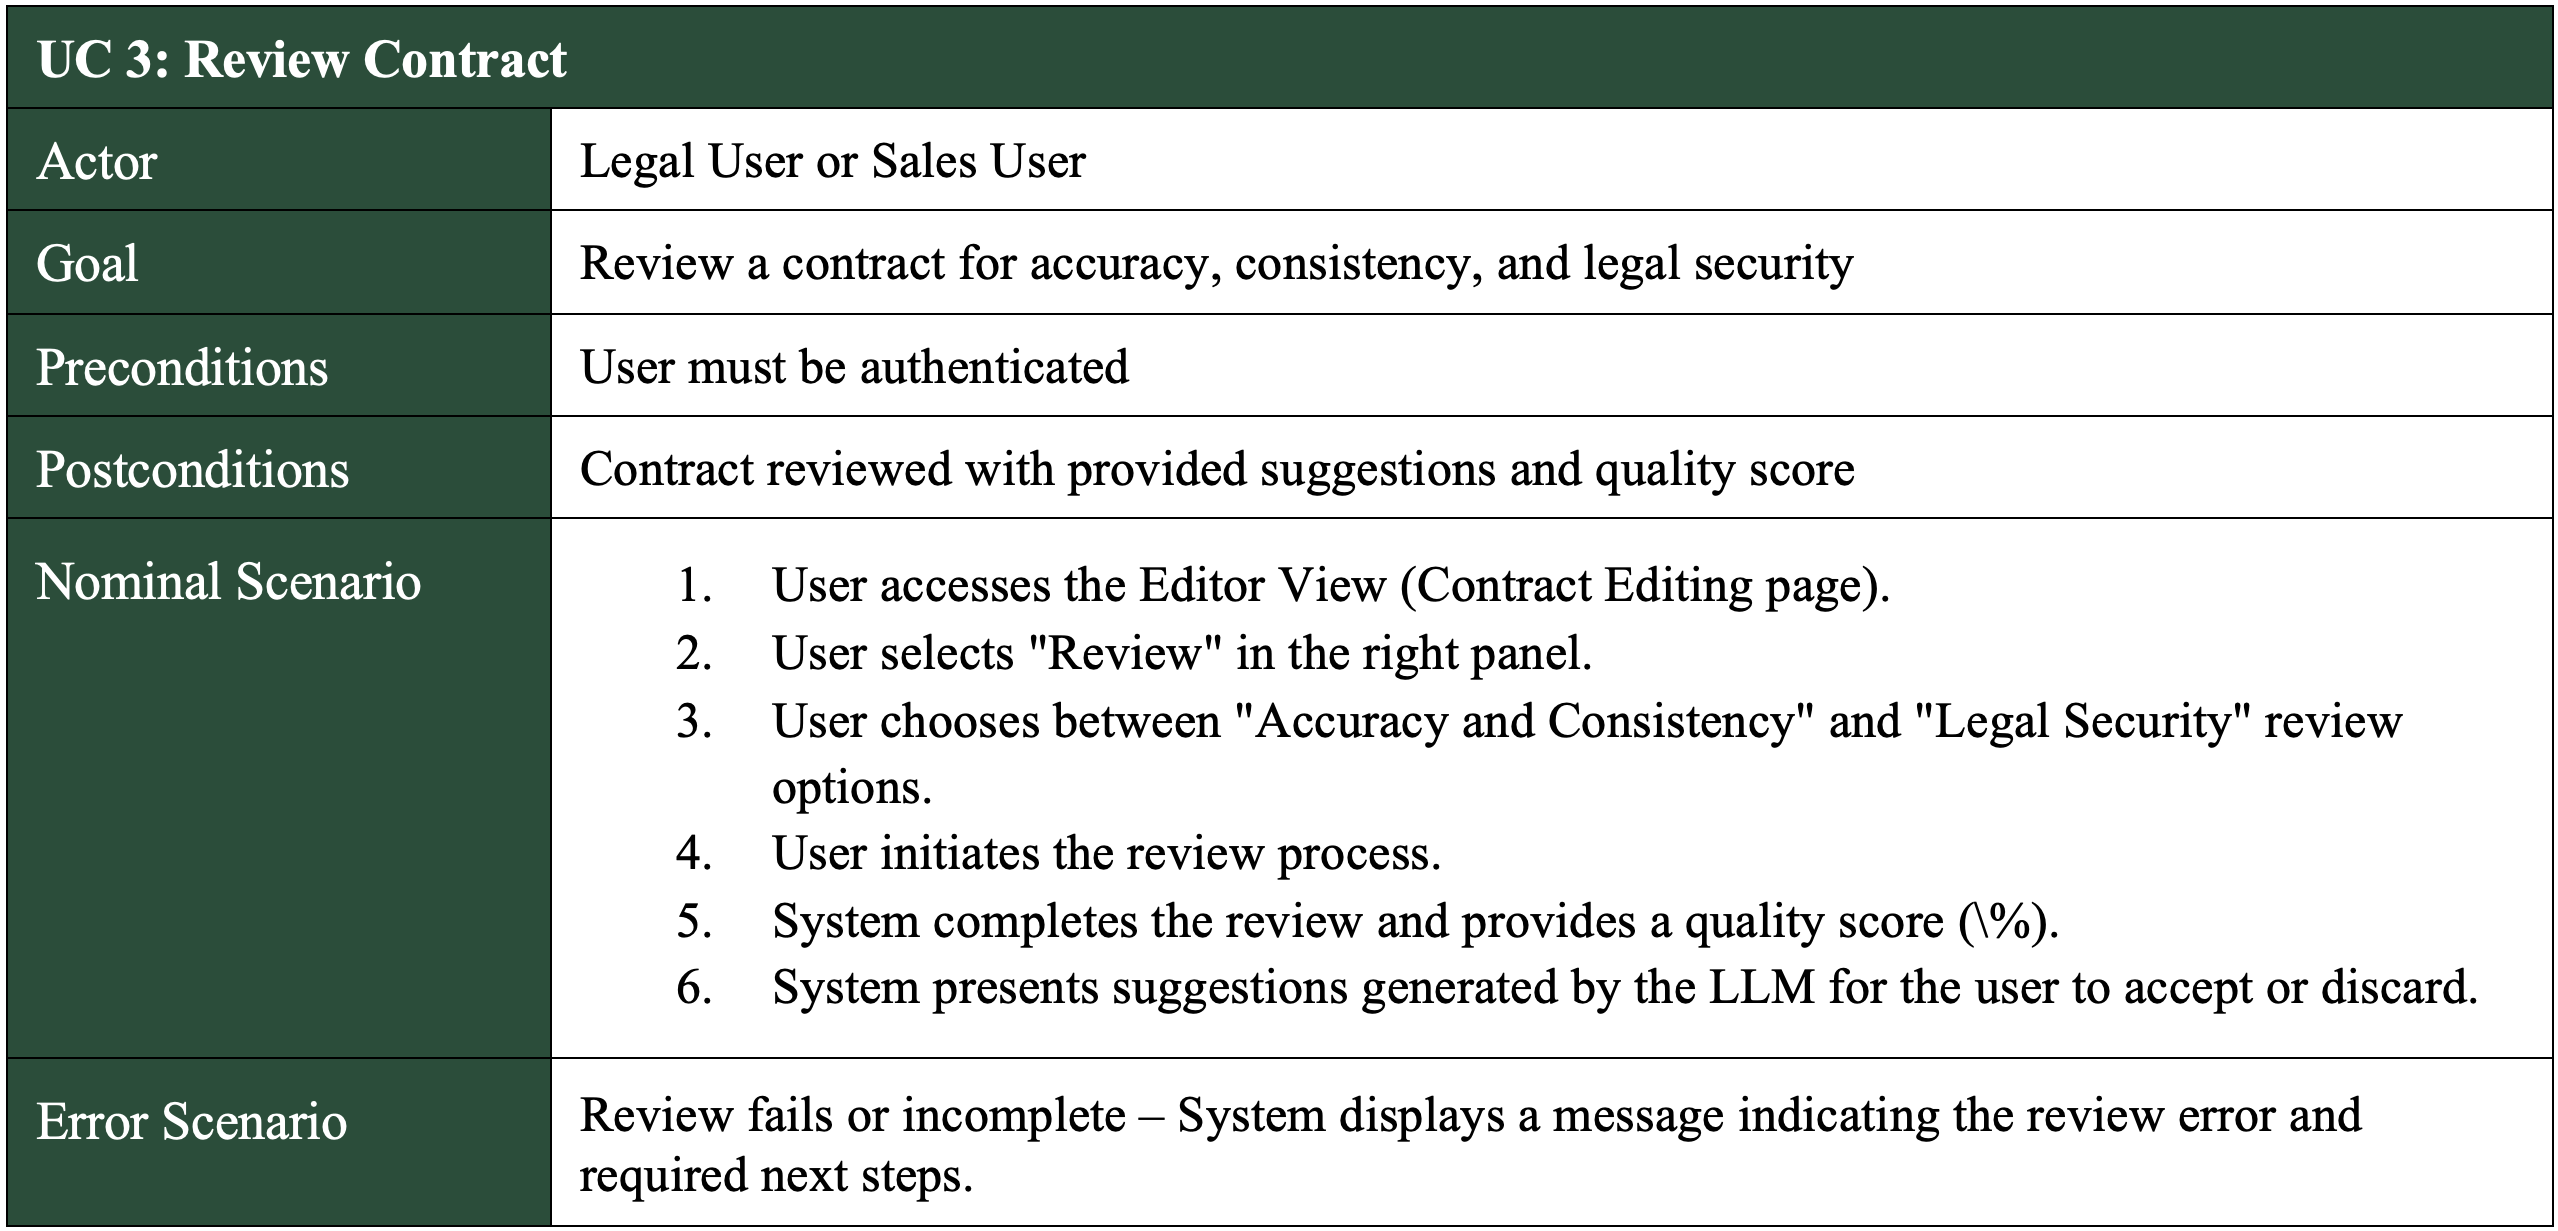
\includegraphics[width=1\textwidth]{Images/Review Contract Use Case.png}
    \captionof{table}{Textual Description of Use Case: Review Contract}
    \label{tab:review_contract_use_case}
\end{center}

% Analysis Sequence Diagram
\subsection{Analysis Sequence Diagram}

\begin{center}
    \centering
    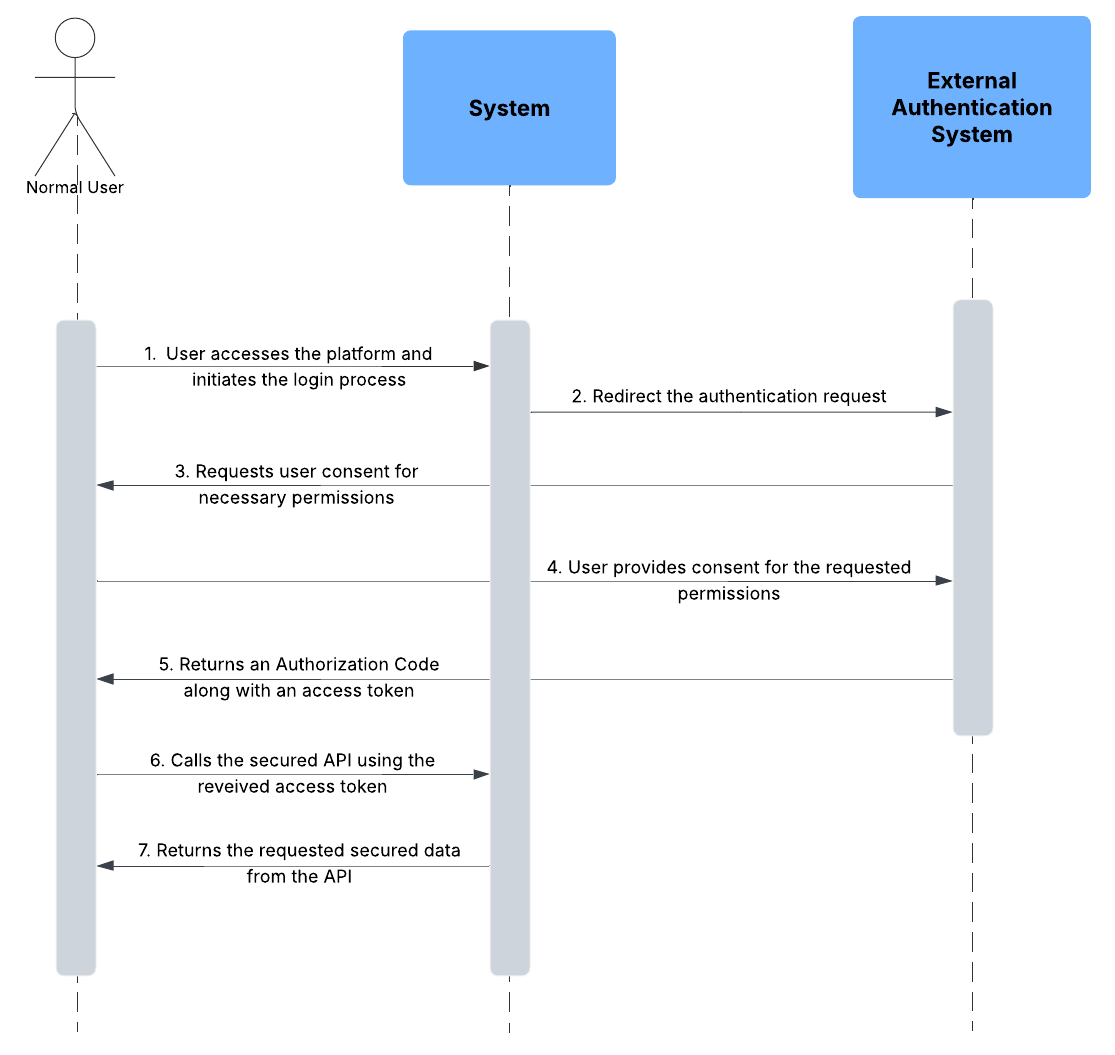
\includegraphics[width=1\textwidth]{Images/Analysis Sequence Diagram.png}
    \captionof{figure}{Analysis Sequence Diagram}
    \label{fig:analysis_sequence_diagram}
\end{center}

The diagram presented above outlines the interaction flow between a normal user intending to authenticate, the main system, and an external authentication system. Initially, the user accesses the platform and clicks on the login button, which prompts the system to redirect the authentication request to the external authentication system. The external authentication system then requests user consent for specific permissions. Upon granting consent by the user, the authentication system issues an authorization code along with an access token back to the system. Finally, the system utilizes this access token to securely call the API and retrieve the requested secured data.

% Constraints and Assumptions
\subsection{Constraints and Assumptions}
To clearly delineate the operational environment and development boundaries, the following constraints and assumptions have been identified:

\textbf{Constraints:}
\begin{itemize}
    \item \textbf{Enterprise Security Compliance}: The system must strictly comply with the organization’s security policies, standards, and regulatory frameworks, ensuring the protection and confidentiality of sensitive contractual and user information.
    \item \textbf{Infrastructure Compatibility}:All technical solutions must be compatible with existing enterprise systems, particularly Azure-based services such as Azure Kubernetes Service (AKS), Azure Entra ID, and Azure PostgreSQL, to ensure seamless integration and minimize disruptions.
    \item \textbf{Cost Efficiency}:The platform must be developed and operated within the allocated budget constraints, adhering to the capacity planning forecasts to optimize resource utilization and cost-effectiveness.
\end{itemize}

\textbf{Assumptions:}
\begin{itemize}
    \item \textbf{Data Availability and Quality}: It is assumed that structured and high-quality data is consistently available from internal sources and third-party integrations to ensure effective AI-driven decision-making.
    \item \textbf{Reliable Cloud Infrastructure}: It is assumed that the Azure cloud infrastructure provides continuous, high-performance service with minimal downtime, ensuring uninterrupted user experiences and workflows.
    \item \textbf{Stable Internet Connectivity}: It is assumed that end users have stable and continuous internet connectivity, enabling consistent access to cloud-hosted services.
    \item \textbf{User Proficiency}: Users are assumed to have a basic level of digital proficiency, enabling them to interact effectively with the intuitive yet sophisticated interfaces provided by the system.
    \item \textbf{Stakeholder Collaboration}: Continuous engagement from all stakeholders, including legal experts, technical teams, and business users, is expected to ensure alignment and smooth progression throughout the project’s lifecycle.
\end{itemize}

% Conclusion
\section{Conclusion}
This chapter detailed the technical rationale behind the project’s approach and identified key enabling technologies. It also defined the system requirements that guide the platform’s architecture, which will be examined in the following chapter.
\minitoc
\label{Chpt:2}
\clearpage


%%%%%%%%%%%%%%%%%%%%%%%%%%%%%%%%%%%%%
%%%%%   Chapitre 3          %%%%%%%%%
%%%%%%%%%%%%%%%%%%%%%%%%%%%%%%%%%%%%%
\chapter{System Architecture and Design}
This chapter explores the detailed architecture and software design of the intelligent contract management platform. It begins with a high-level overview of the system’s structure, covering frontend, backend, and AI components. The integration of LLMs via LangChain and advanced editing through Tiptap is also discussed. The logical designs of backend and frontend modules are illustrated. Finally, the chapter presents UML diagrams to clarify class structures and workflow interactions.\mynewline

The architectural elements and components presented in this chapter reflect the broader system context in which the internship was carried out; however, the descriptions are limited to areas in which I was directly involved or contributed during the project.

\newpage
\fancyhead[R]{\textsc{Chapter 3 - System Architecture and Design}}
\hypertarget{thirdchapter}{}

%% Architecture of the Solution
\section{Solution's Architecture}

% Overall Architecture
\subsection{Overall Architecture}
\begin{center}
    \centering
    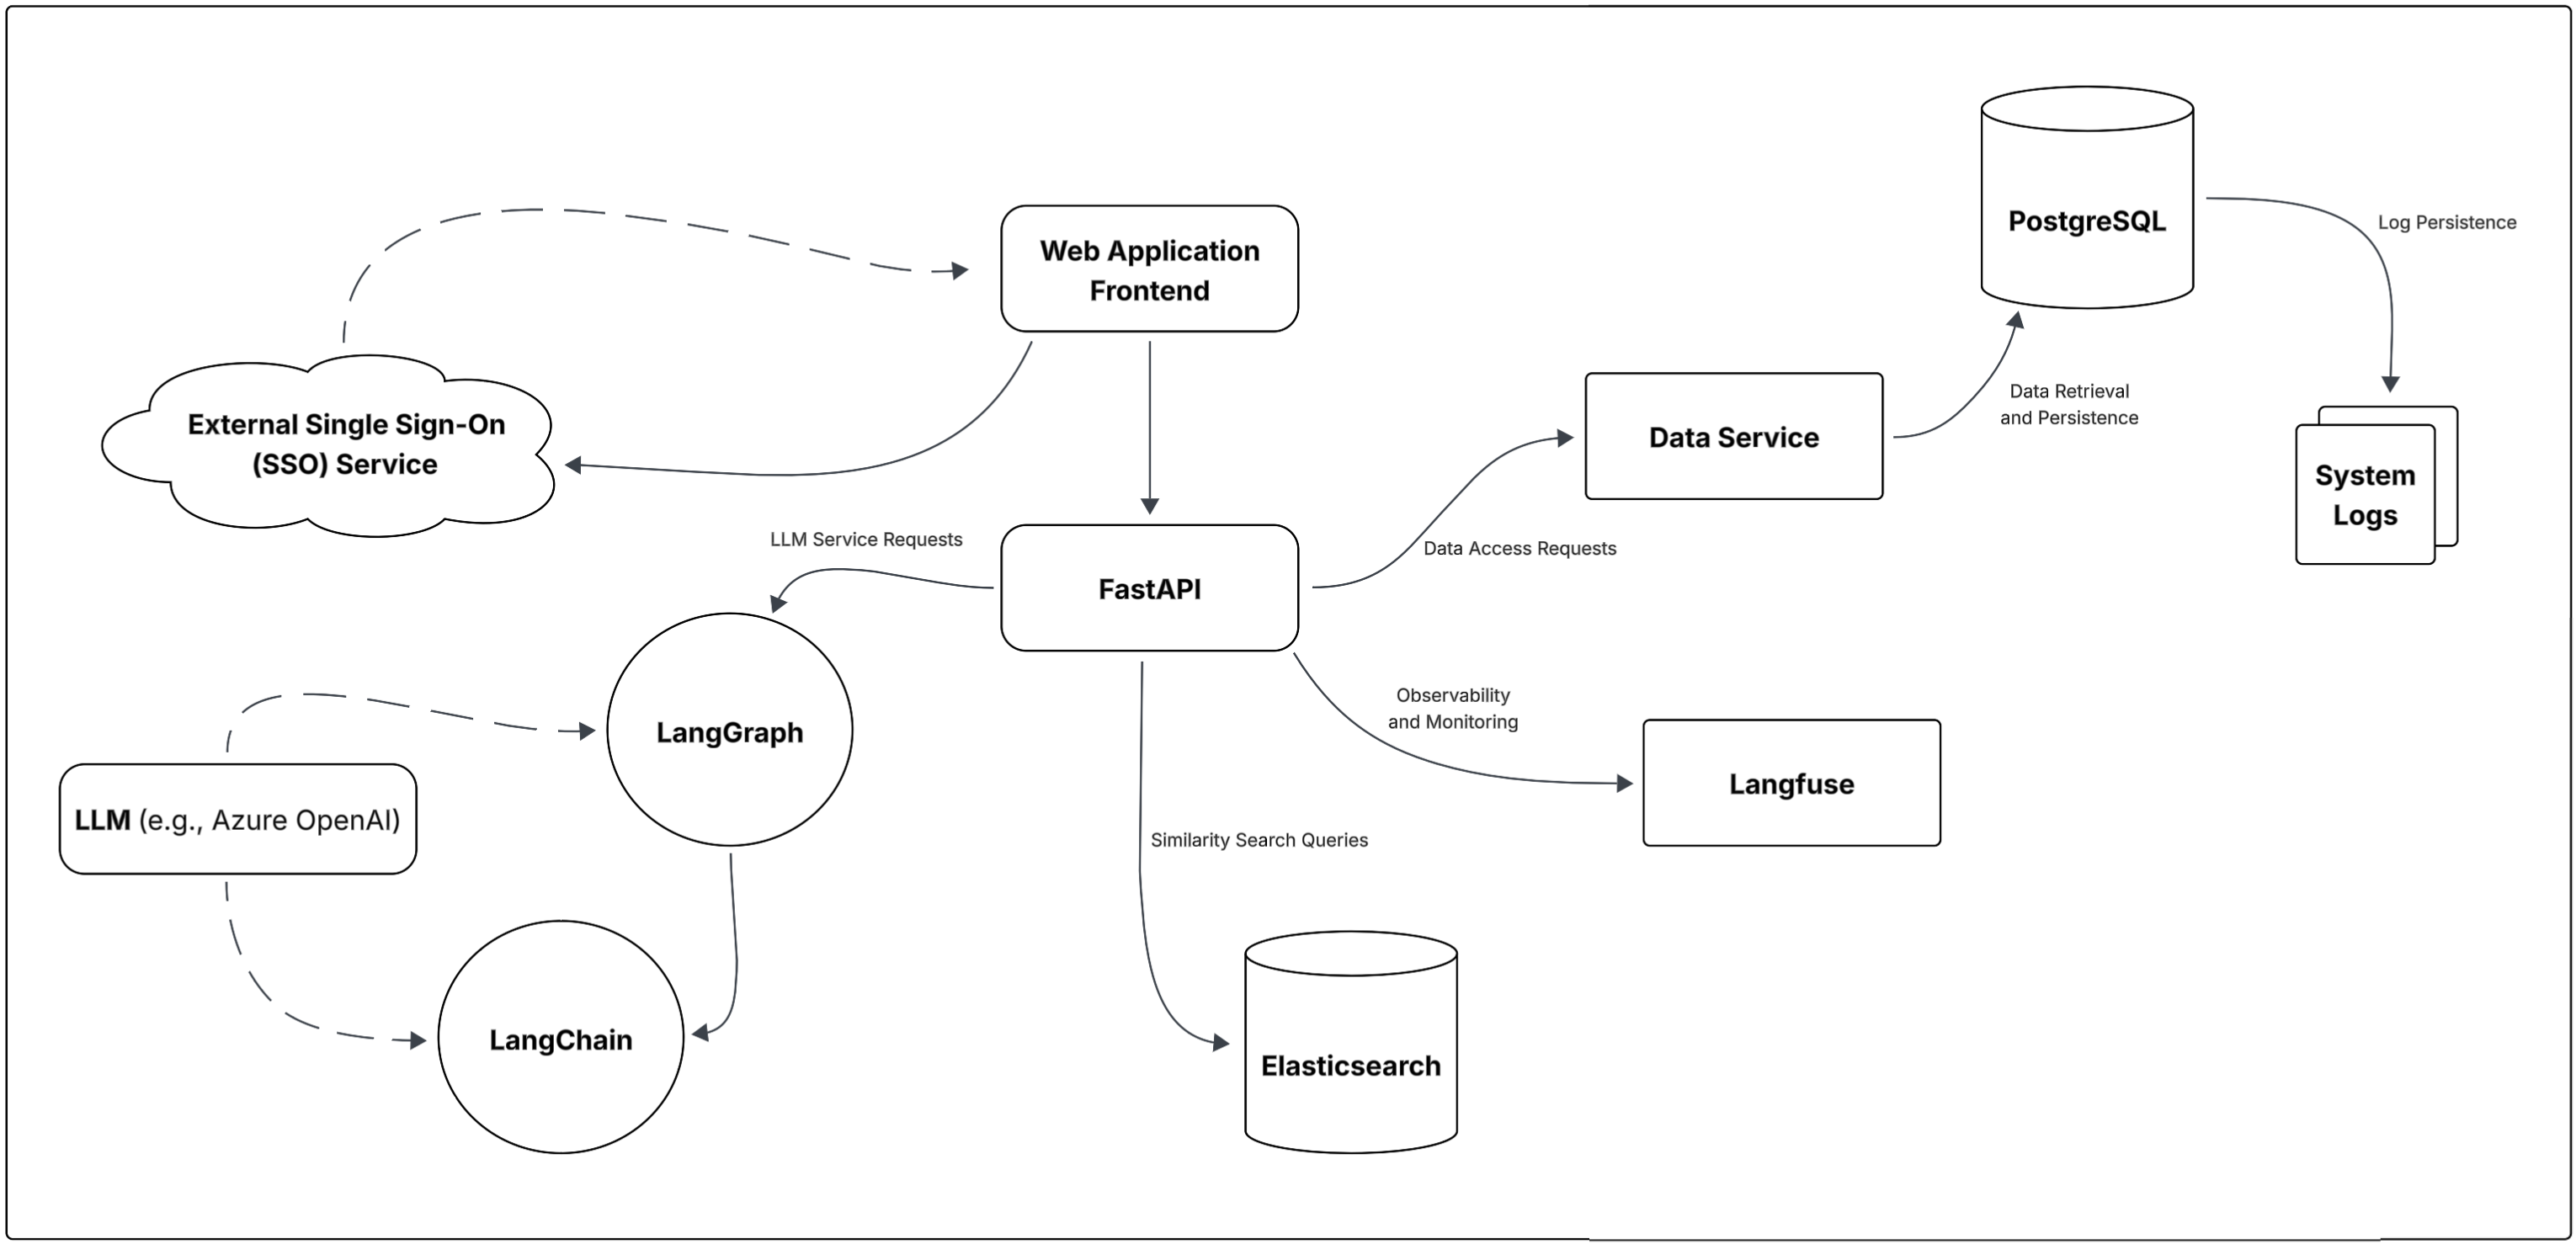
\includegraphics[width=1\textwidth]{Images/Global Architecture of the Platform.png}
    \captionof{figure}{Overall Architecture of the Platform}
    \label{fig:overall_architecture}
\end{center}

The overall architecture of the platform, as illustrated in Figure \ref{fig:overall_architecture}, depicts a structured interaction between users, frontend interfaces, backend services, databases, and AI-driven components. Users interact with the platform primarily through the web application frontend. Depending on the access requirements, users may need to authenticate via an external Single Sign-On (SSO) service to securely access private functionalities or can directly access public features like shared links through URL-based token authentication.\mynewline

The frontend communicates with the backend services built using the FastAPI framework, where the core business logic resides. This backend interacts extensively with a PostgreSQL database to persist logs and manage structured data efficiently. Elasticsearch is implemented as a vector database responsible for similarity searches, enhancing the platform’s data retrieval capabilities.\mynewline

Interaction with various Large Language Models (LLMs)—including Azure OpenAI, OpenAI GPT-4.1, and Anthropic—is managed via the LangChain framework, abstracting and simplifying communications and integration. LangGraph extends LangChain’s capabilities, facilitating the execution of complex, graph-based AI agent workflows, thereby enabling more dynamic interactions and decision-making processes within the platform.\mynewline

For observability and monitoring purposes, the system integrates Langfuse. Langfuse provides comprehensive tracking of all interactions with LLM APIs, including essential metrics such as API response times, token usage, and associated costs. This observability ensures robust management and operational transparency of the AI services integrated within the platform.

% Logical Architecture
\subsection{Logical Architecture}
This section presents the internal structure of the application codebase. Given that the core mission focused on the implementation of new features across both the backend service and frontend, the focus here will be on the logical design of these two key components.

% Main Backend Service
\subsubsection{Main Backend Service}
In the FastAPI-based backend, we adopted a layered modular architecture for each functional domain. As illustrated in Figure~\ref{fig:backend_module_architecture}, each module is composed of a controller responsible for managing HTTP and WebSocket requests, which communicates with a service layer that encapsulates the business logic. The service interacts with the data models and relies on DTOs (Data Transfer Objects) for structured data exchanges across layers.\mynewline

To abstract and streamline access to persistent storage, a DAO (Data Access Object) pattern is implemented. The DAO interfaces with a dedicated Data Service layer that encapsulates direct database operations. This clear separation of responsibilities ensures high maintainability, testability, and scalability. It also allows for improved consistency in query logic and facilitates secure data access patterns.\mynewline

This architecture was particularly beneficial for implementing legal use cases and AI-enhanced features, where the backend needed to efficiently orchestrate data retrieval, validation, and transformation between internal components and the frontend interface.

\begin{center}
    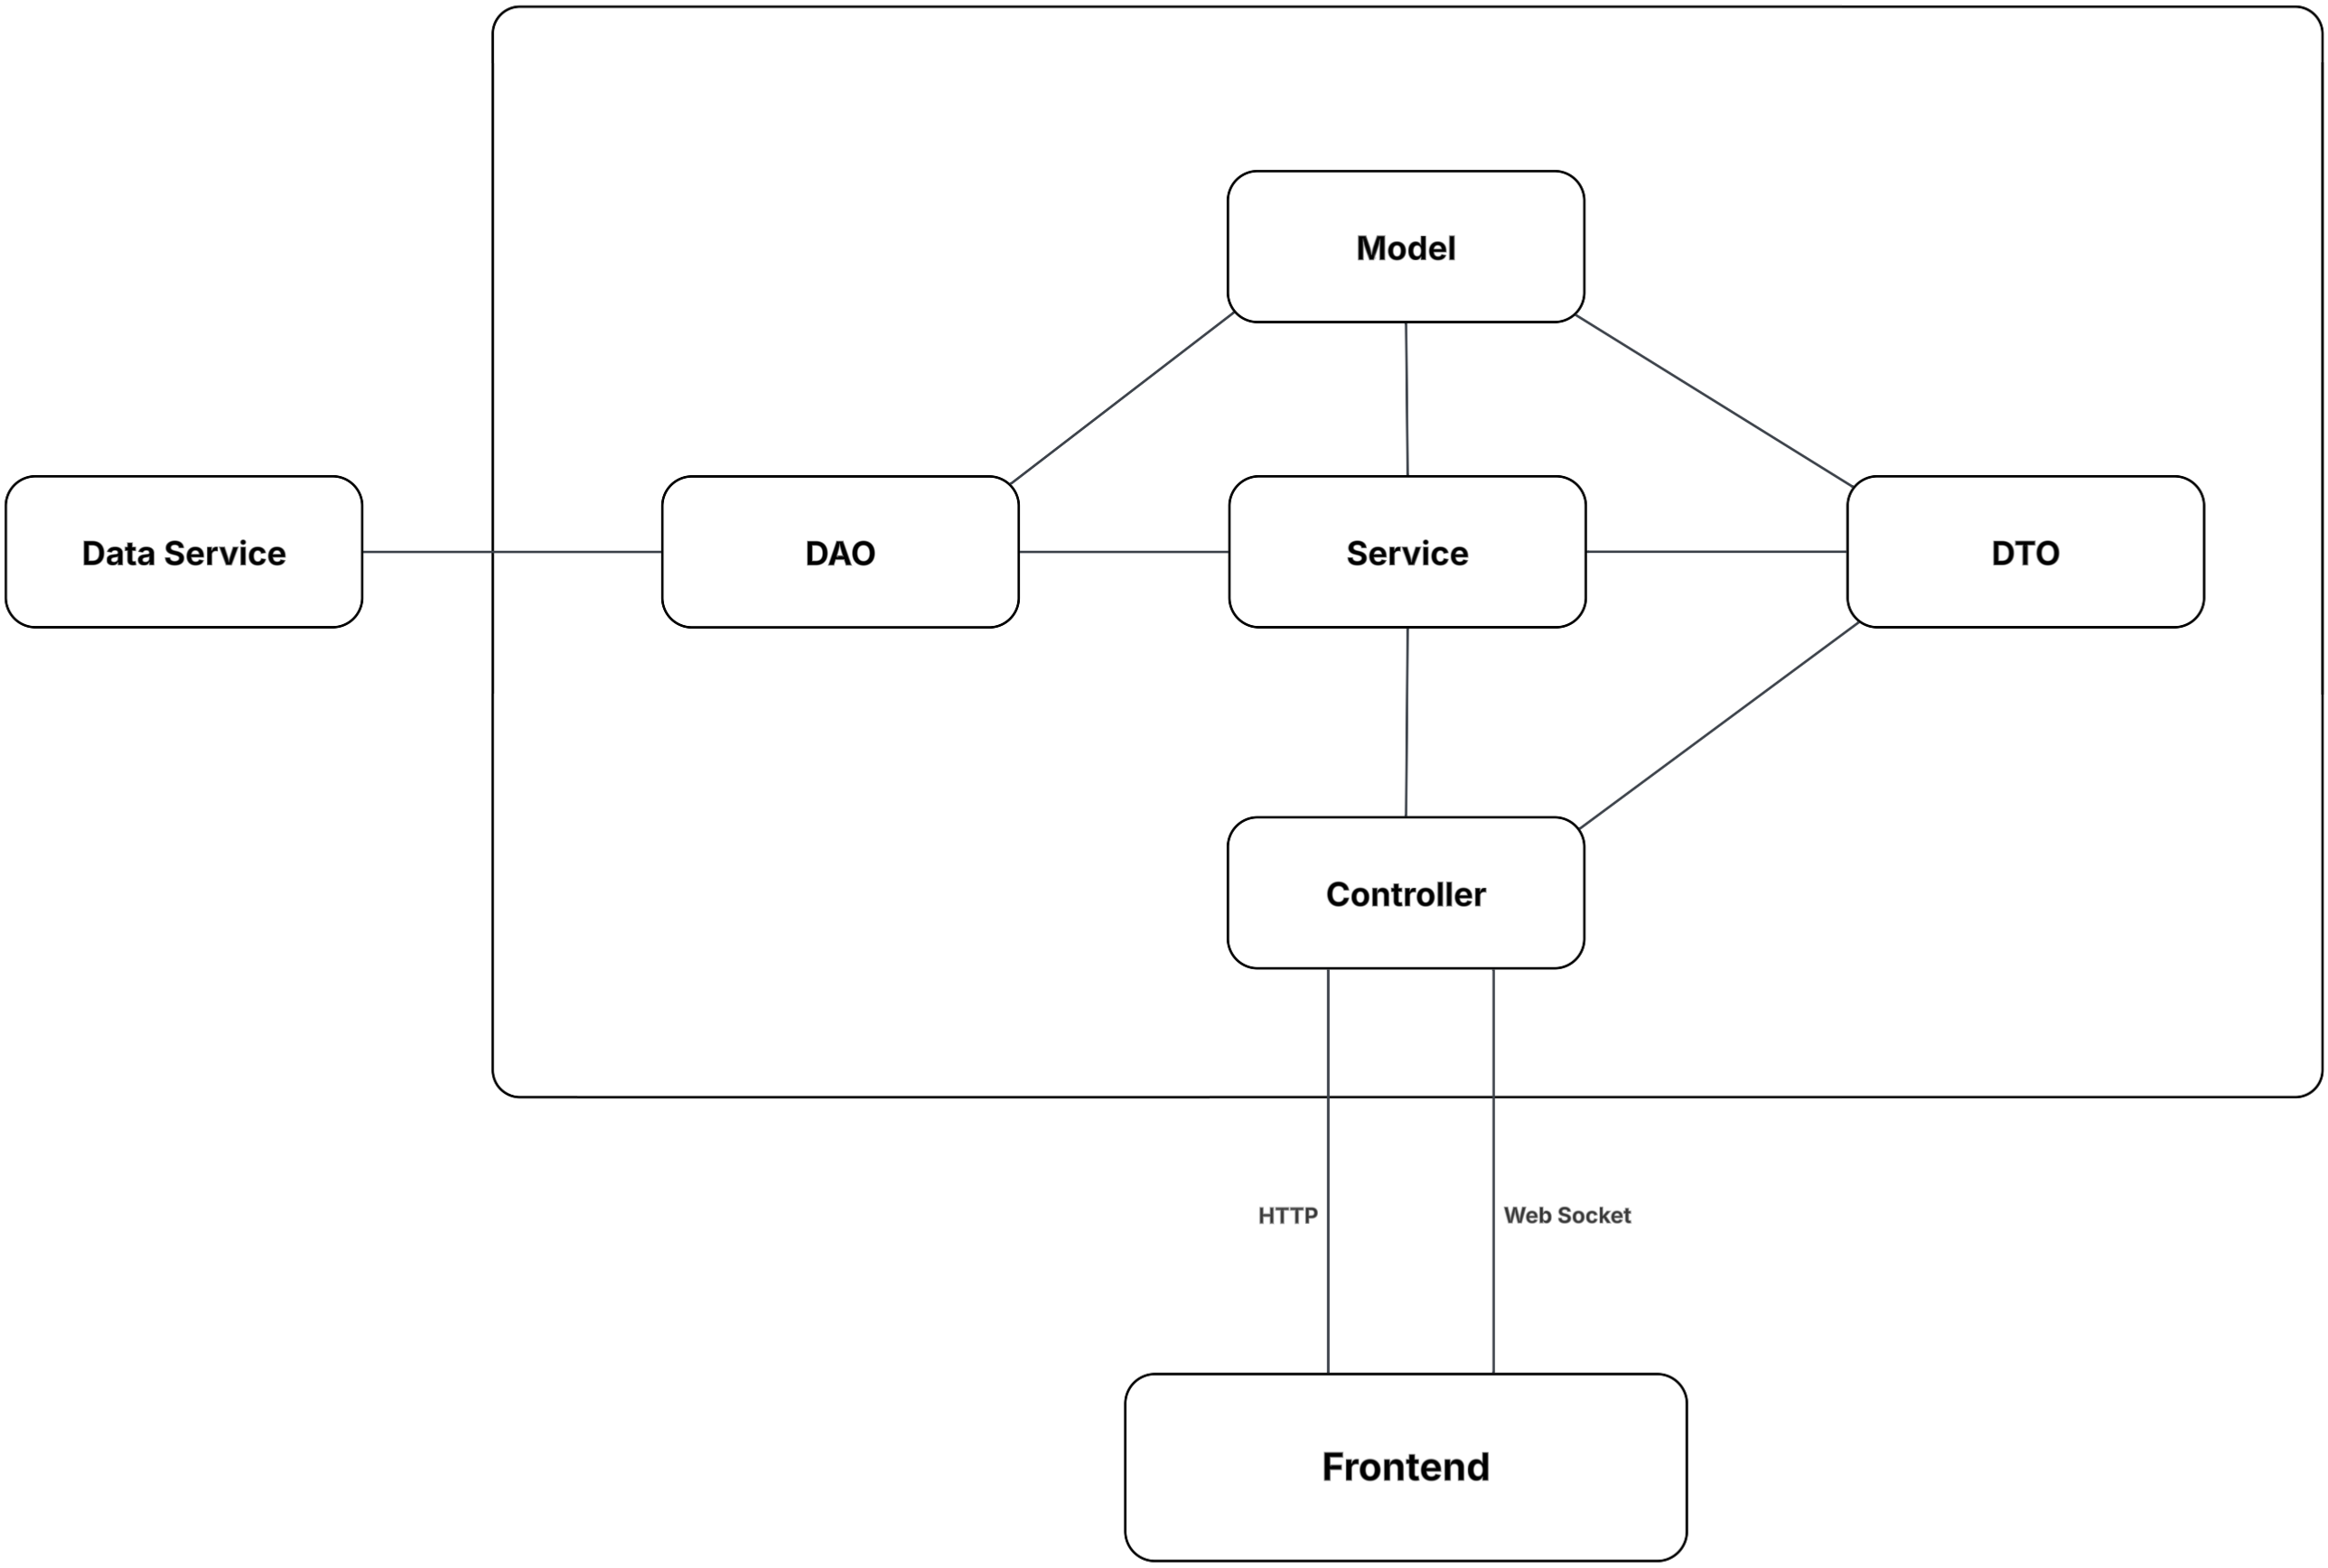
\includegraphics[width=0.95\textwidth]{Images/Layered Architecture of a Backend Module.png}
    \captionof{figure}{Layered Architecture of a Backend Module}
    \label{fig:backend_module_architecture}
\end{center}

% Frontend Structure
\subsubsection{Frontend Structure}
On the frontend side, we implemented a modular structure grounded in the principles of separation of concerns and component reusability. As shown in Figure~\ref{fig:frontend_module_architecture}, each module consists of components responsible for managing the user interface and interactions, and services that encapsulate domain-specific business logic and handle communication with the backend via HTTP or WebSocket, depending on the context.\mynewline

The architecture also integrates a dedicated store layer to manage state, especially for dynamic content and session-persistent interactions. DTOs are used to structure and validate data exchanged with the backend, while models represent the internal structure of application entities.\mynewline

This modular organization promotes code maintainability and scalability, enabling independent development and testing of each module. It also facilitates a smooth integration of new features such as AI-based clause recommendations and real-time collaboration within the contract editor.

\vspace{0.3cm}

\begin{center}
    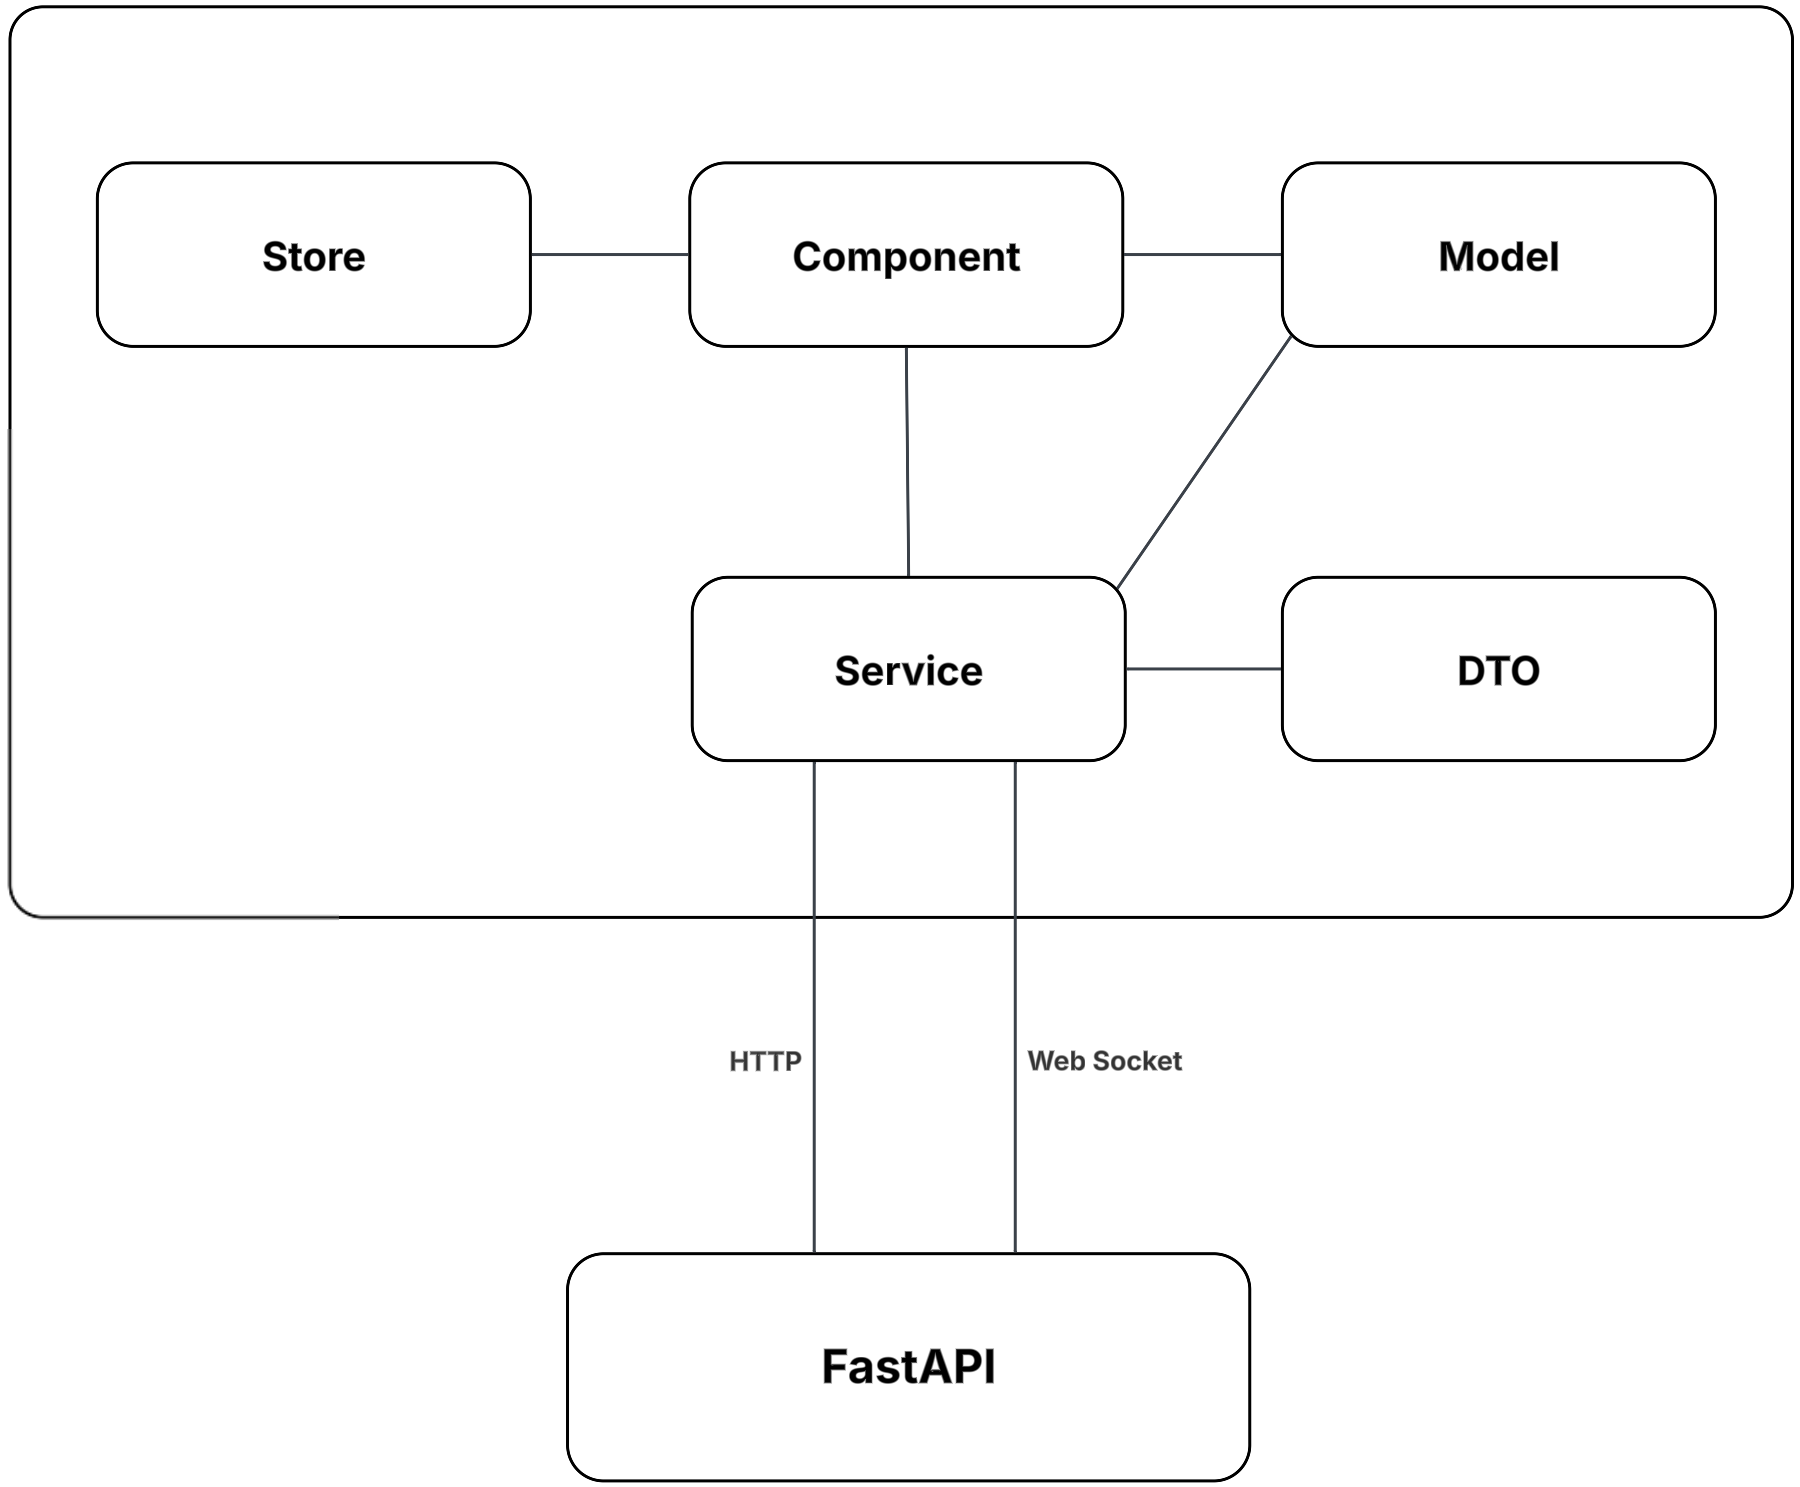
\includegraphics[width=0.7\textwidth]{Images/Component Architecture of a Frontend Module.png}
    \captionof{figure}{Component Architecture of a Frontend Module}
    \label{fig:frontend_module_architecture}
\end{center}

% LLM Integration
\subsection{LLM Integration}
Integration of LLMs within the platform is streamlined using the LangChain framework, which provides an abstraction layer to interact uniformly with multiple LLM providers. As depicted in Figure \ref{fig:llm_integration}, this integration allows the platform to remain flexible, accommodating advancements in LLM technologies with minimal architectural adjustments.\mynewline

\begin{center}
    \centering
    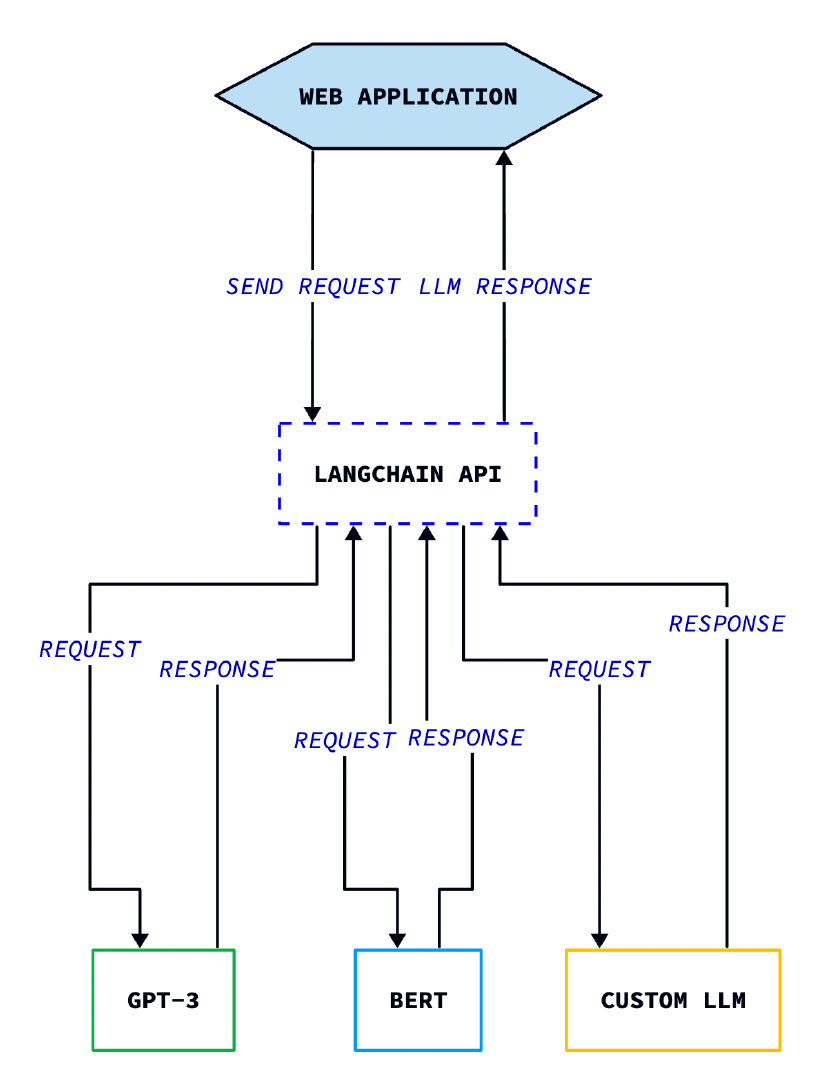
\includegraphics[width=0.55\textwidth]{Images/LLM Integration.png}
    \captionof{figure}{LLM Integration via LangChain}
    \label{fig:llm_integration}
\end{center}

LangChain efficiently manages the interaction between the platform and various LLM services, handling data flow optimization, API call management, input/output formatting, and robust error handling mechanisms. It also incorporates rate-limiting functionalities to ensure resource-efficient and cost-effective interactions.


% Text Editing Framework: Tiptap
\subsection{Text Editing Framework: Tiptap}
On the frontend, the platform employs the Tiptap editor—an open-source, third-party framework built on top of ProseMirror and designed to provide extensible rich-text editing capabilities, especially within modern React-based applications. Tiptap is integrated as a ready-to-use library rather than being developed in-house, and its adoption ensures robust and reliable document editing features aligned with best practices in frontend architecture.\mynewline

Within the platform, Tiptap has been tailored specifically for the structured editing of legal documents such as contracts. Unlike traditional rich-text editors, Tiptap is configured to meet the complex formatting and regulatory requirements intrinsic to legal documents. Users can efficiently organize document elements into legally defined sections, clauses, and subsections.\mynewline

Tiptap supports critical legal editing features, including:

\begin{itemize}
    \item \textbf{Structured Document Editing}: Customized nodes and marks for legally compliant structural elements, allowing users to efficiently manage and format contracts according to legal and organizational standards.
    \item \textbf{Clause and Variable Management}: Specialized nodes for inserting, editing, and managing clauses and dynamic contract variables directly within the document, ensuring precision and consistency.
    \item \textbf{Real-time Collaborative Editing}: Integration with collaborative technologies such as Y.js enables multiple legal professionals and stakeholders to simultaneously edit, review, and approve documents, reflecting changes in real-time and maintaining a clear audit trail of modifications.
\end{itemize}

This tailored configuration of Tiptap significantly enhances the user experience, providing a robust, intuitive interface optimized specifically for drafting, reviewing, and finalizing complex legal contracts, while leveraging an established and actively maintained framework from the open-source ecosystem.

\begin{center}
    \centering
    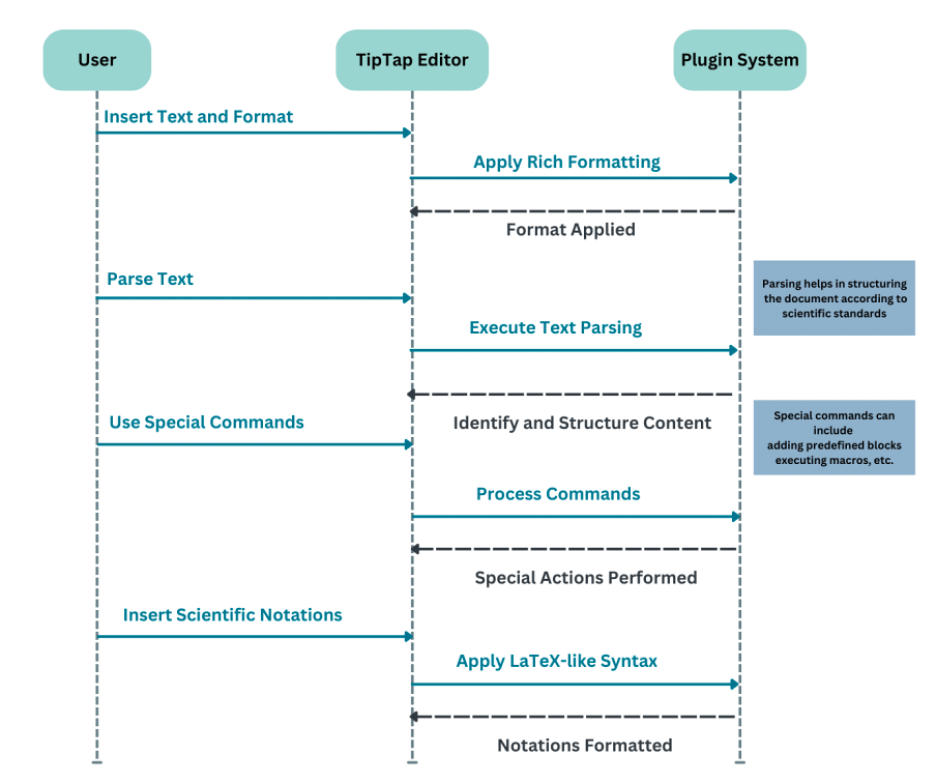
\includegraphics[width=0.9\textwidth]{Images/Tiptap Editing Framework.png}
    \captionof{figure}{Tiptap Text Editing Framework for Legal Documents}
    \label{fig:tiptap_legal_framework}
\end{center}

% Detailed Design
\section{Detailed Design}

% Class Diagram
\subsection{Class Diagram}
The class diagram is a fundamental UML diagram type that illustrates the static structure of the software system, detailing its classes, their attributes, methods, and the relationships among these classes. Figure \ref{fig:class_diagram} presents the comprehensive class diagram of the intelligent contract management platform developed during this internship.

\begin{landscape}
\begin{figure}[H]
    \centering
    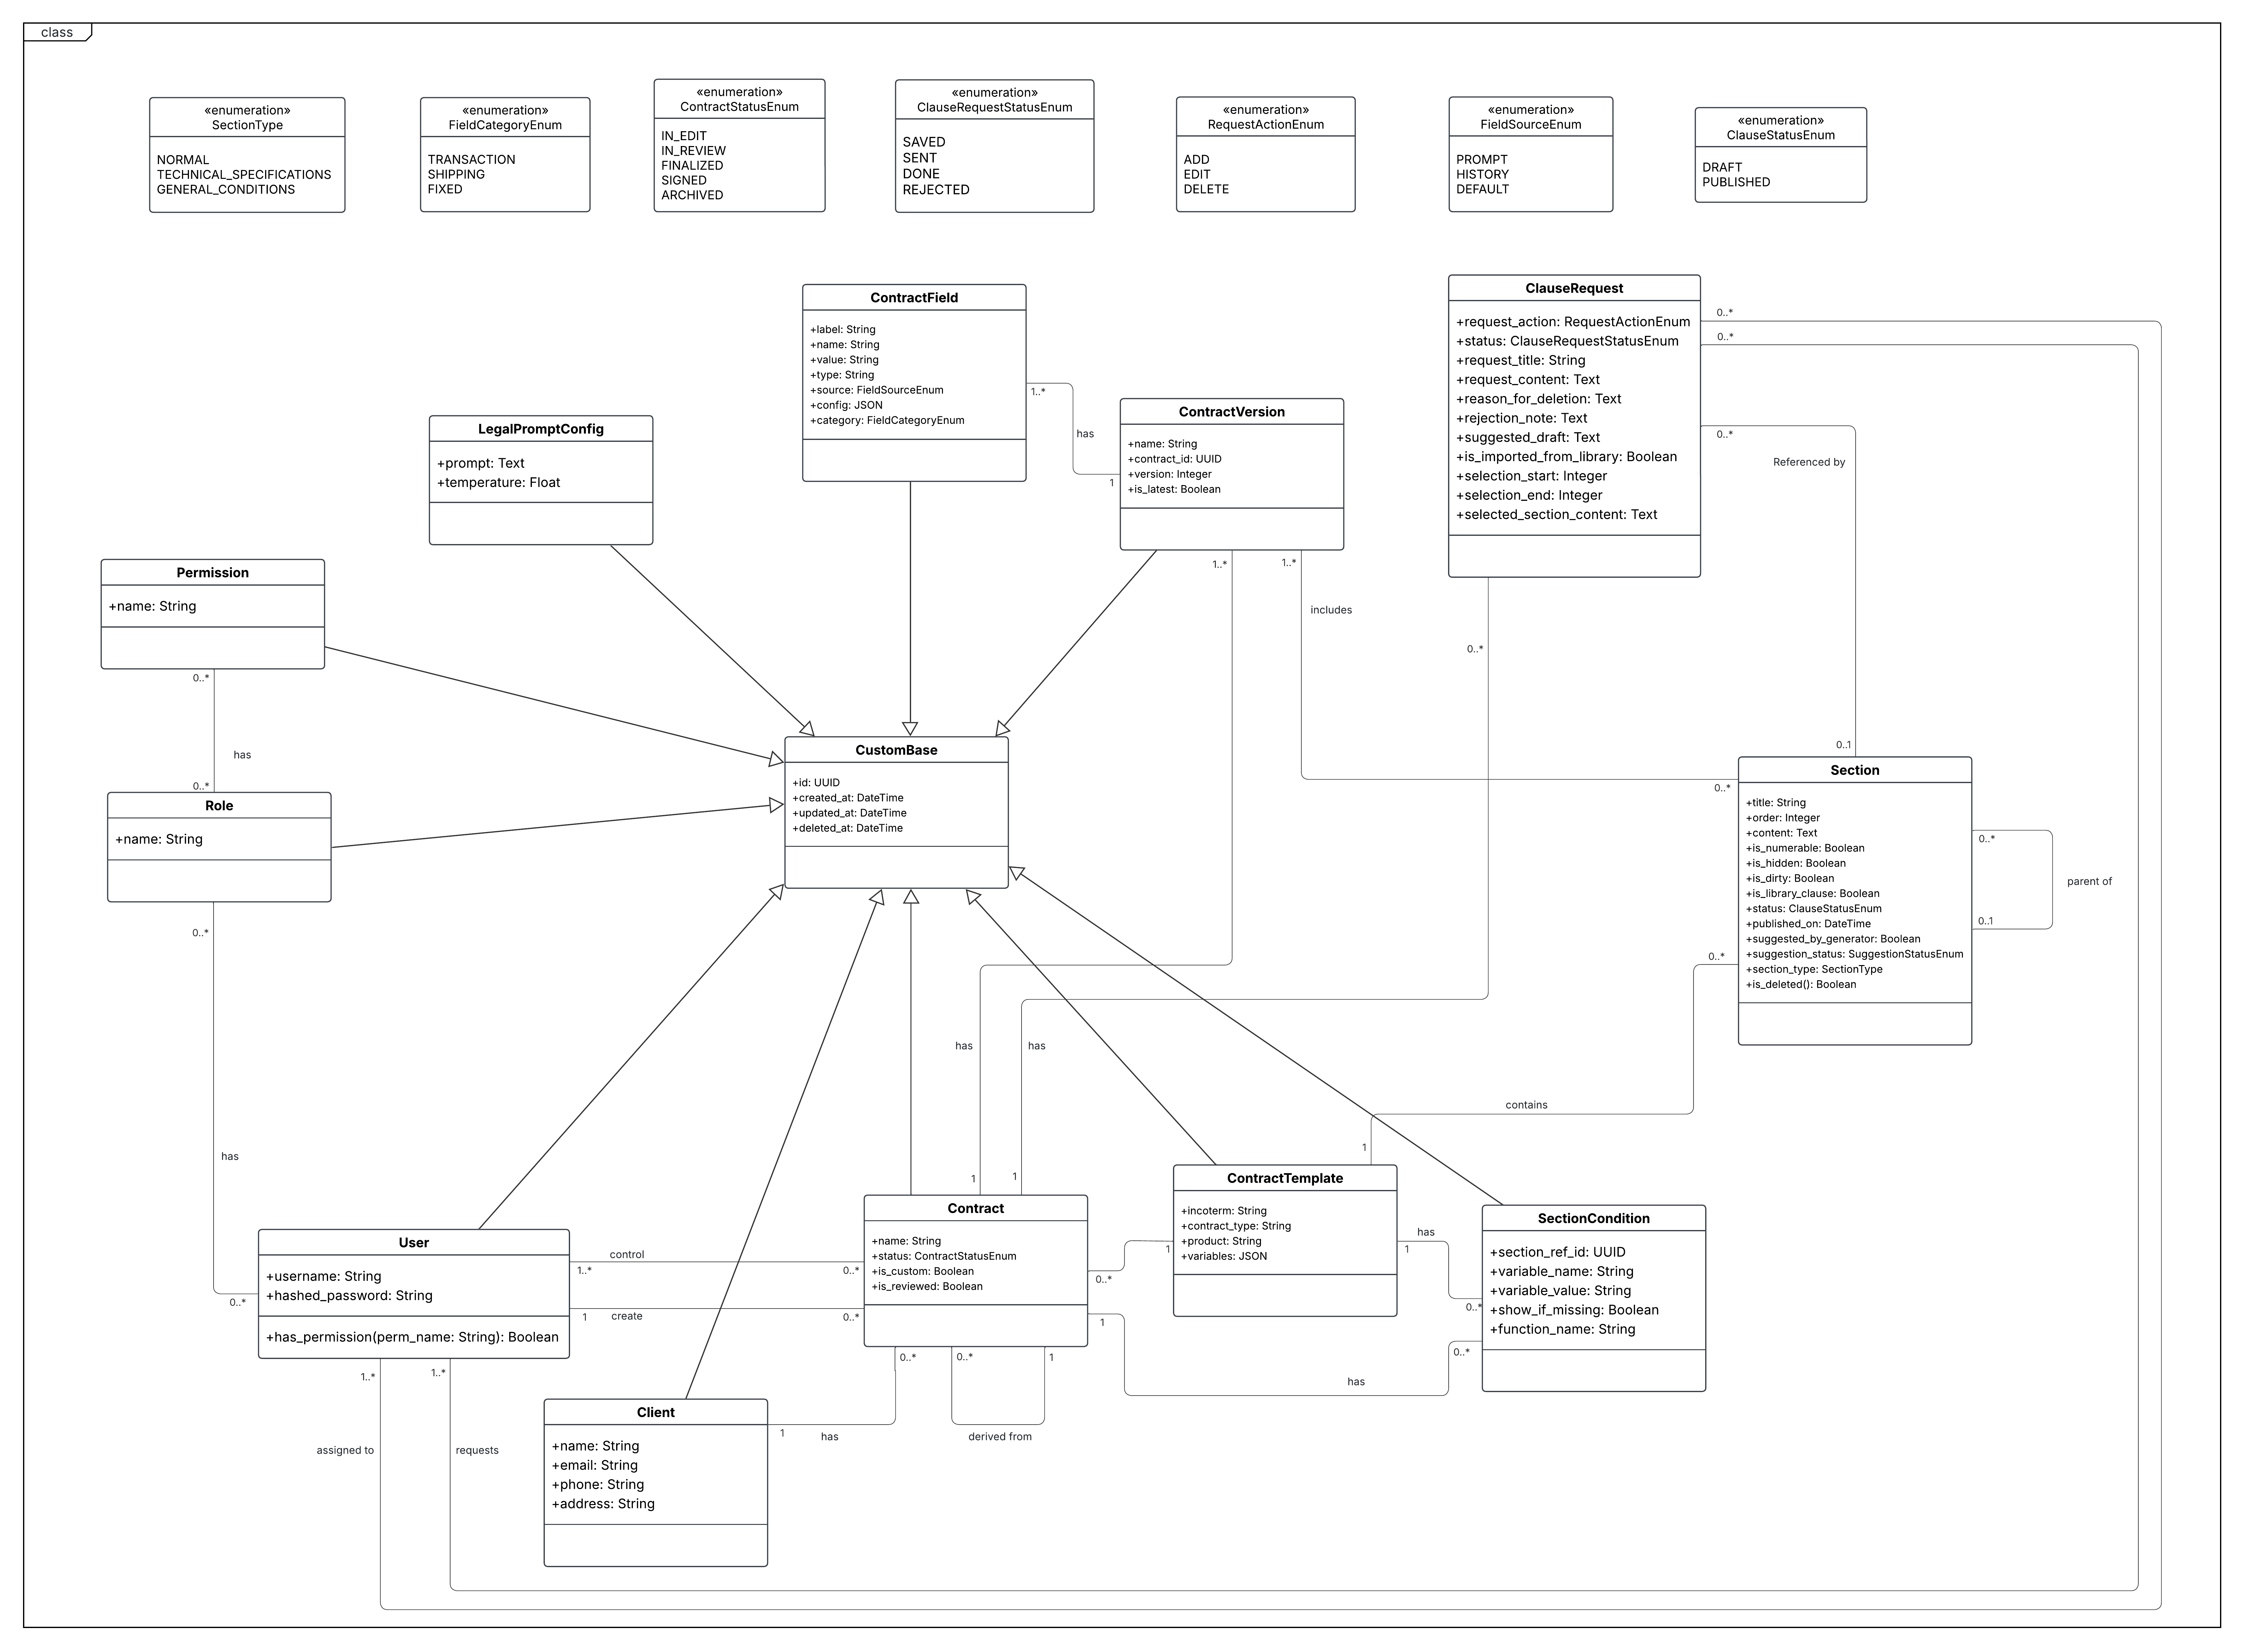
\includegraphics[width=1.2\textwidth]{Images/Class Diagram.png}
    \caption{Class Diagram of The Platform}
    \label{fig:class_diagram}
\end{figure}
\end{landscape}

All classes in this architecture inherit from the \textbf{CustomBase}, providing universal attributes such as a unique identifier (\textit{id}), timestamps for creation, update, and deletion of entries.\mynewline

The \textbf{User} class represents users of the platform, associating each user with specific \textbf{Roles} (e.g., Sales or Legal), which determine a set of \textbf{Permissions} defining accessible functionalities.\mynewline

The \textbf{Contract} class represents an agreement between a company and its client, distinct from the platform users. Each contract is associated with a specific \textbf{Client}, and relies on a \textbf{ContractTemplate} based on a combination of product, contract type, and Incoterm. Contracts can also originate by cloning existing contracts.\mynewline

Contracts feature five distinct statuses represented by the enumeration \textit{ContractStatusEnum}:

\begin{itemize}
    \item \textbf{IN\_EDIT}: Initial stage, editable by both Sales and Legal teams.
    \item \textbf{IN\_REVIEW}: Editable by Legal, but frozen for Sales, acting as a proxy to finalization.
    \item \textbf{FINALIZED}: Fully reviewed and locked from editing by both teams.
    \item \textbf{SIGNED}: Confirmed and mutually agreed upon by the company and the client.
    \item \textbf{ARCHIVED}: Used for historical purposes based on the company's archiving policies.
\end{itemize}

Each \textbf{Contract} is composed of one or multiple \textbf{ContractVersions} to manage iterative changes and improvements. Versions include structured \textbf{Sections}, each comprising multiple fields detailed by \textbf{ContractField} classes representing variables specific to each contract section.\mynewline

The \textbf{ClauseRequest} class is specifically dedicated to handling clause modification requests made by Sales users to the Legal team, marked by statuses within the \textit{ClauseRequestStatusEnum} (\textit{SAVED}, \textit{SENT}, \textit{DONE}, \textit{REJECTED}). Requests transition from \textit{SAVED} when initially drafted by a Sales user, to \textit{SENT} upon submission to Legal. Depending on the decision by Legal, these requests become \textit{DONE} upon acceptance and implementation, or \textit{REJECTED} if not approved.\mynewline

This class diagram provides a clear and structured representation, highlighting crucial entities, their interrelations, and functionalities integral to the platform’s effective management of digital contract operations.


% Detailed Sequence Diagram
\subsection{Detailed Sequence Diagram}
Following the analysis phase where chronological interactions between the system and actors were outlined, detailed sequence diagrams have been created. These diagrams precisely illustrate interactions among system components to realize specific use cases. The use cases chosen for detailed representation are \textbf{Generate a New Contract}, \textbf{Create Clause Request} and \textbf{Review Clause Request}.

% Generate a New Contract
\subsubsection{Generate a New Contract}

\begin{center}
    \centering
    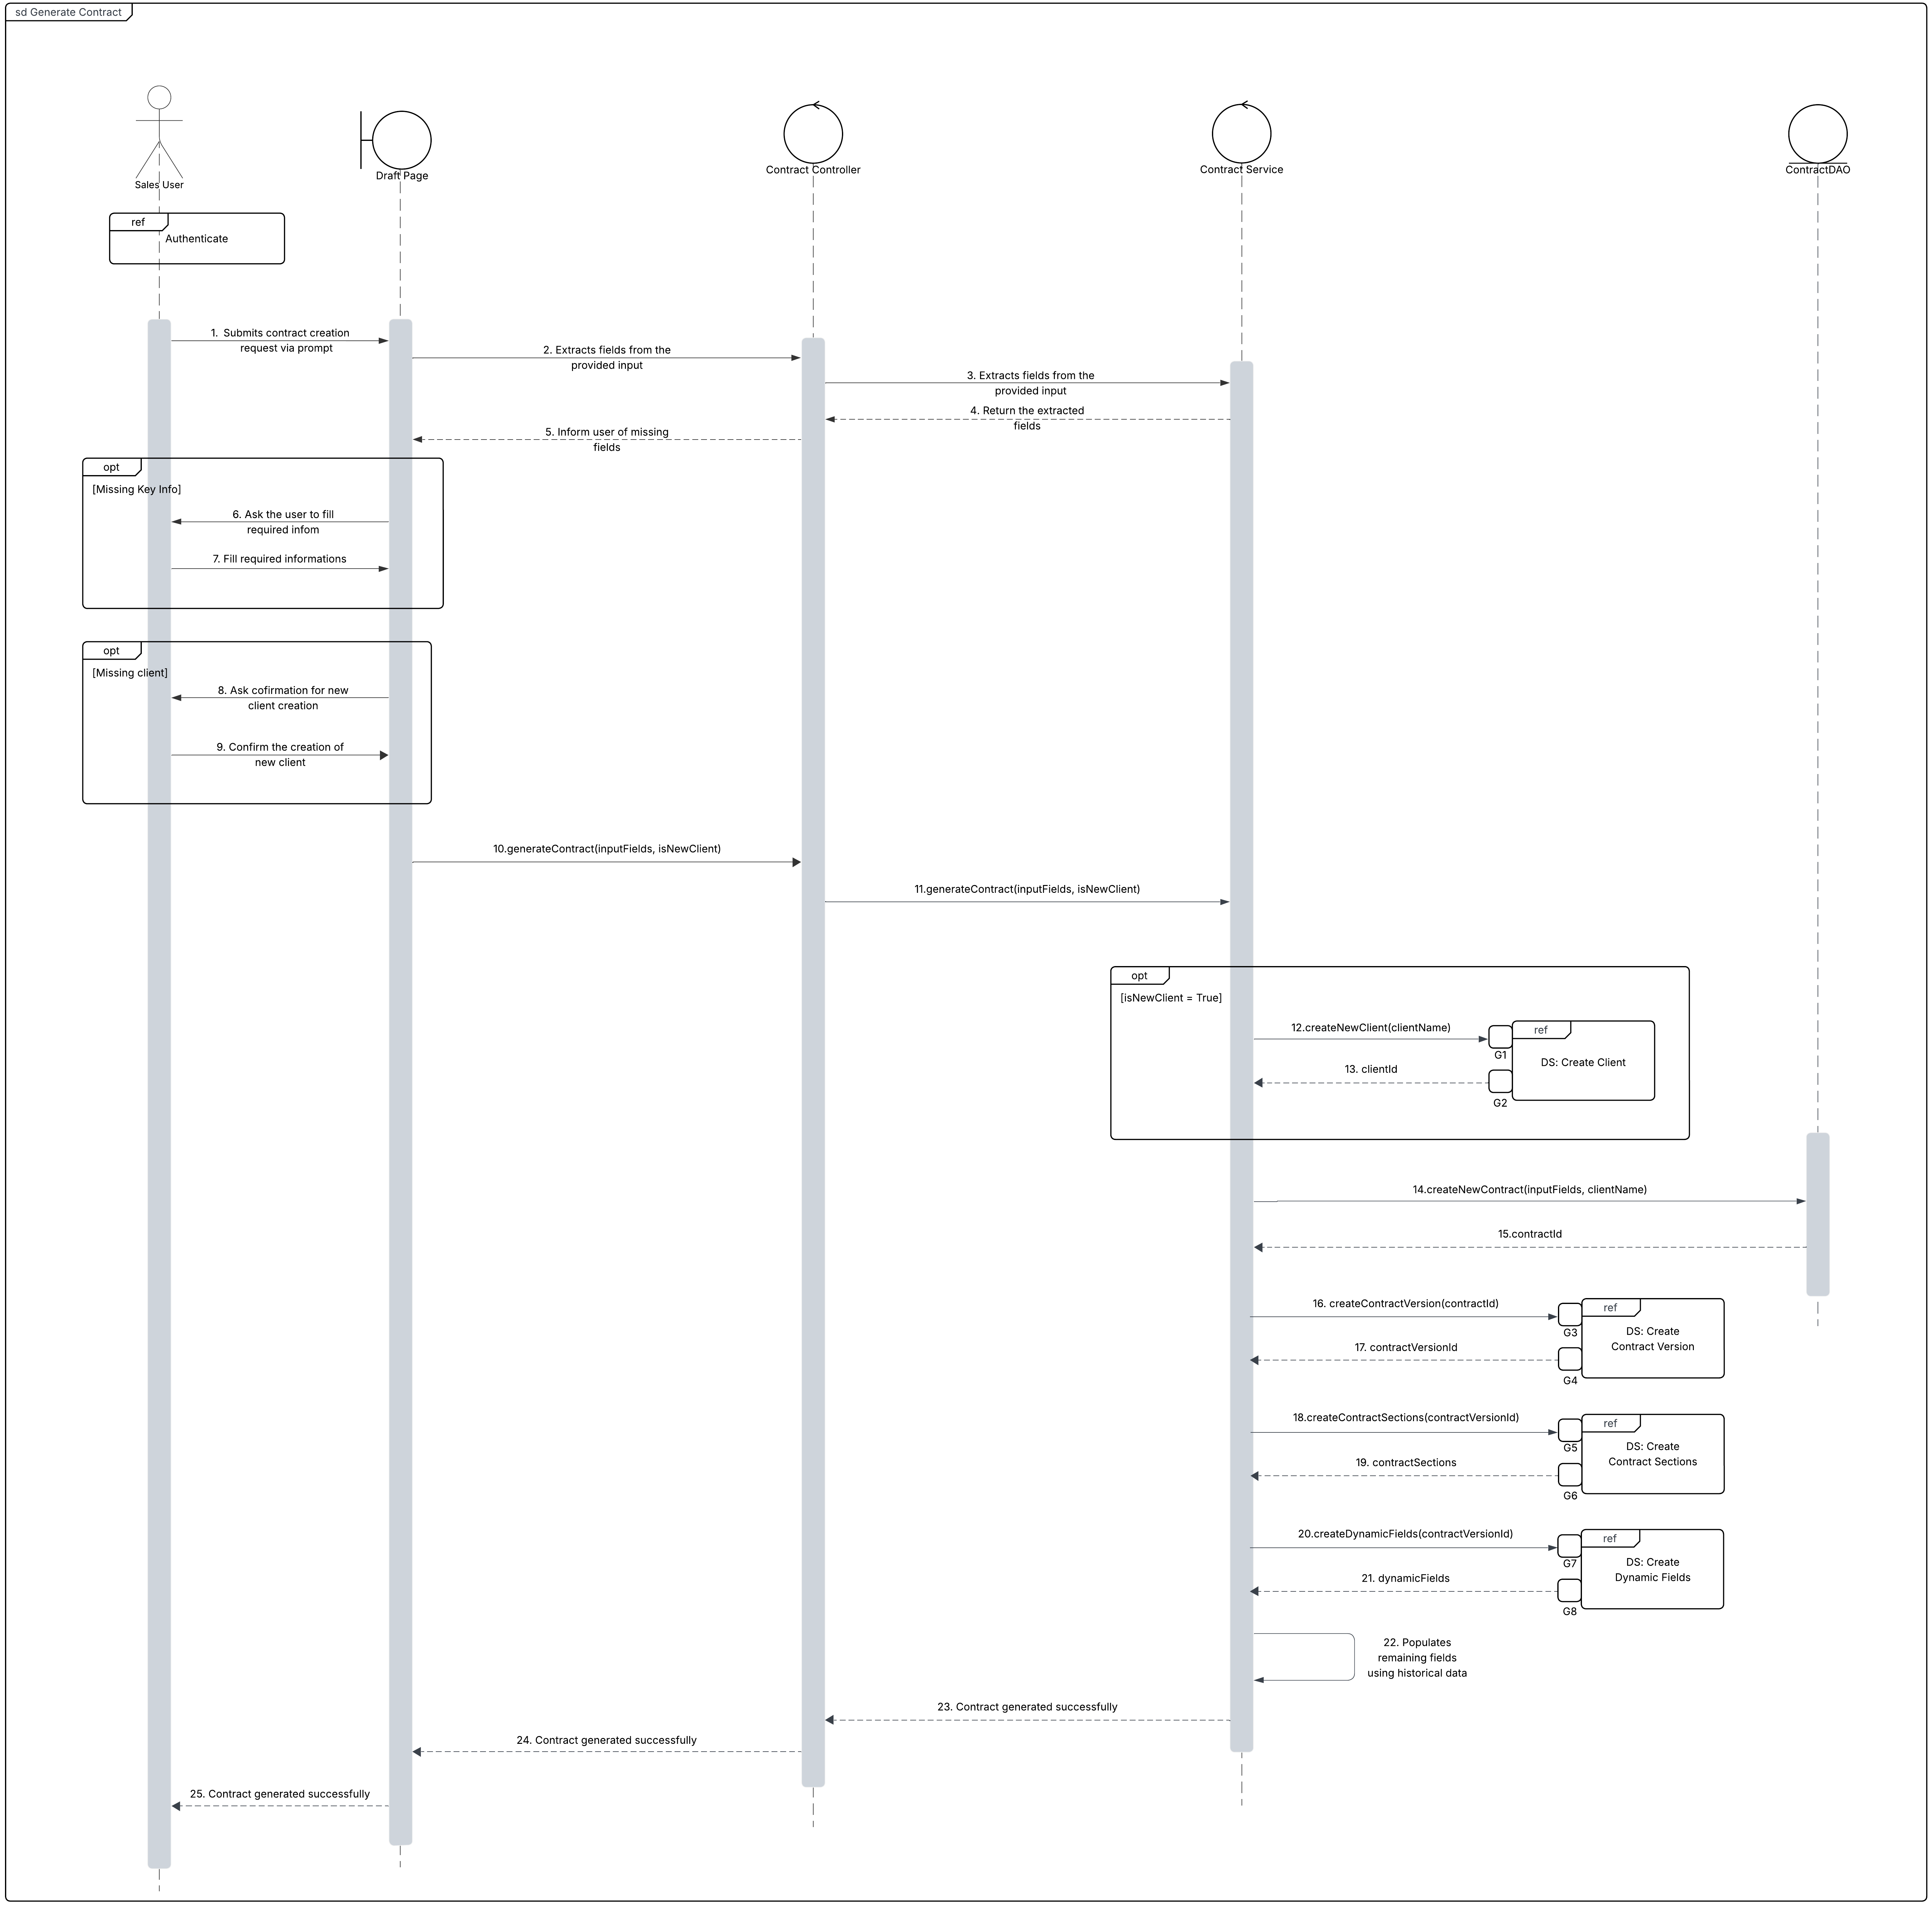
\includegraphics[width=1\textwidth]{Images/Sequence Diagram - Draft Contract.png}
    \captionof{figure}{Sequence Diagram - Draft Contract}
    \label{fig:sequence_diagram_draft_contract}
\end{center}

To maintain clarity and reduce complexity, certain subprocesses—such as Create Client and Create Contract Version—are encapsulated within ref frames. The detailed sequence diagrams for these referenced interactions are provided in the following figures:

\begin{figure}[H]
    \centering

    \begin{minipage}[t]{0.48\textwidth}
        \centering
        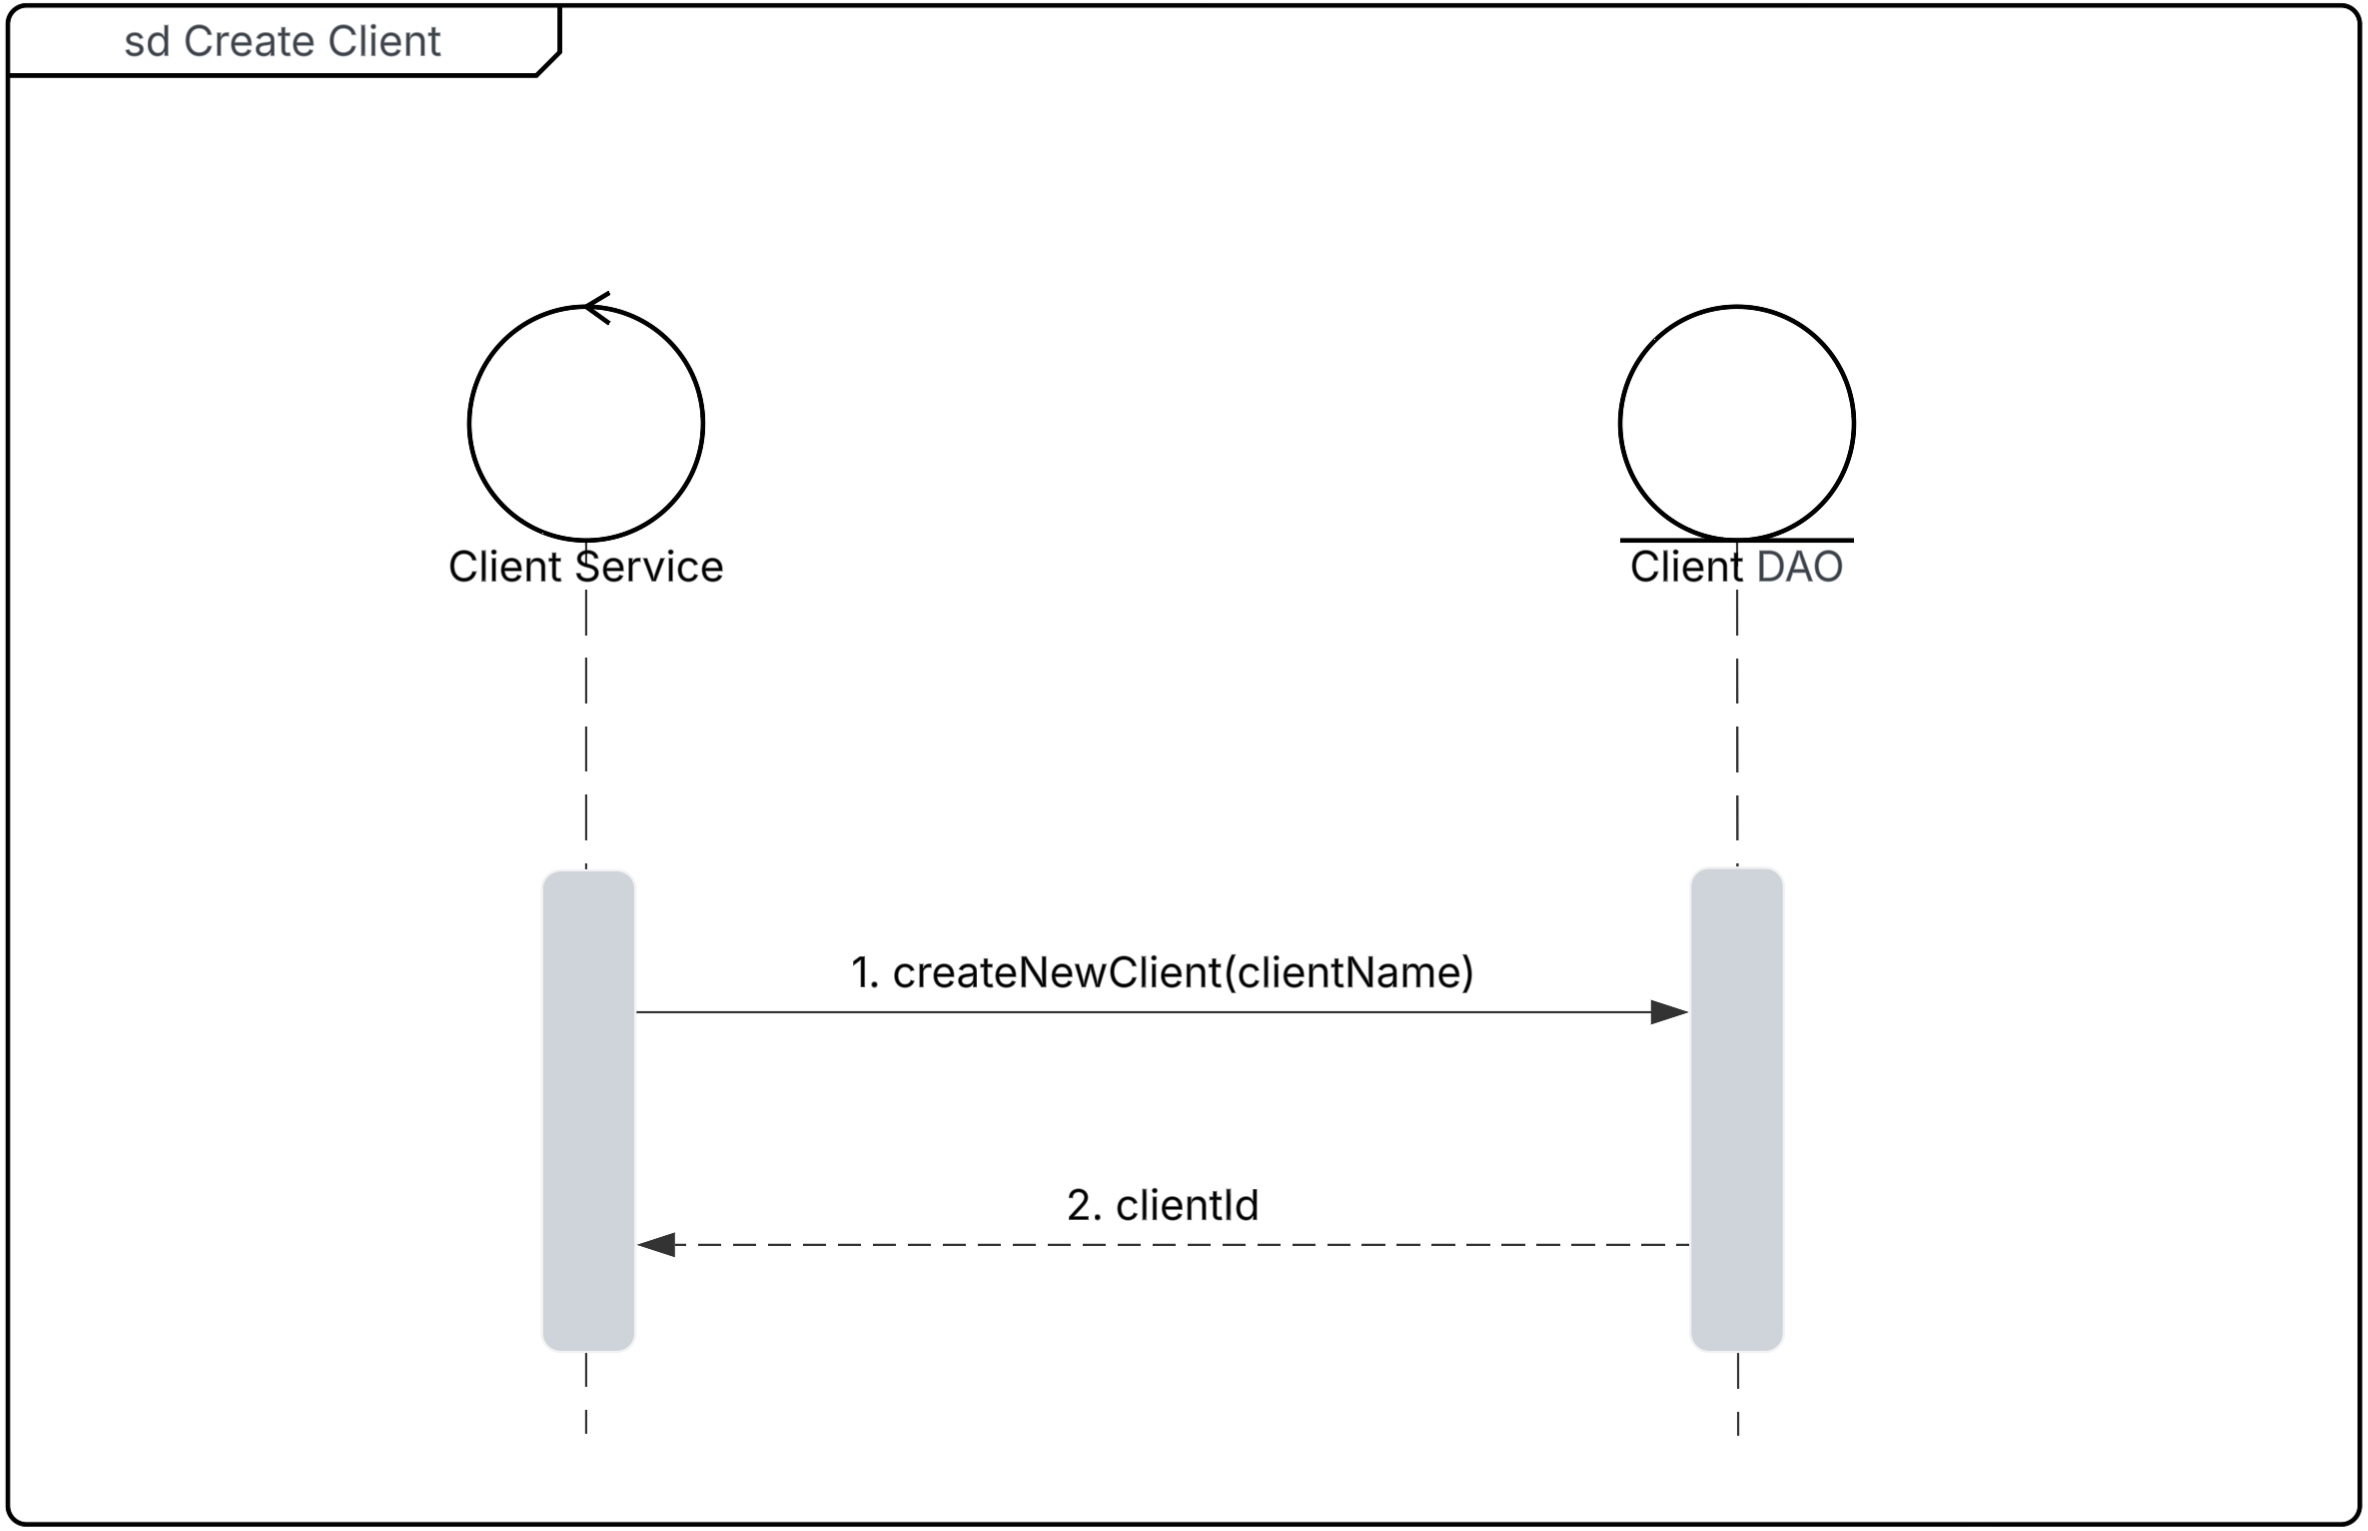
\includegraphics[width=\textwidth]{Images/Sequence Diagram - Create Client Ref.png}
        \captionof{figure}{Sequence Diagram – Create Client}
        \label{fig:sequence_diagram_create_client}
    \end{minipage}
    \hfill
    \begin{minipage}[t]{0.48\textwidth}
        \centering
        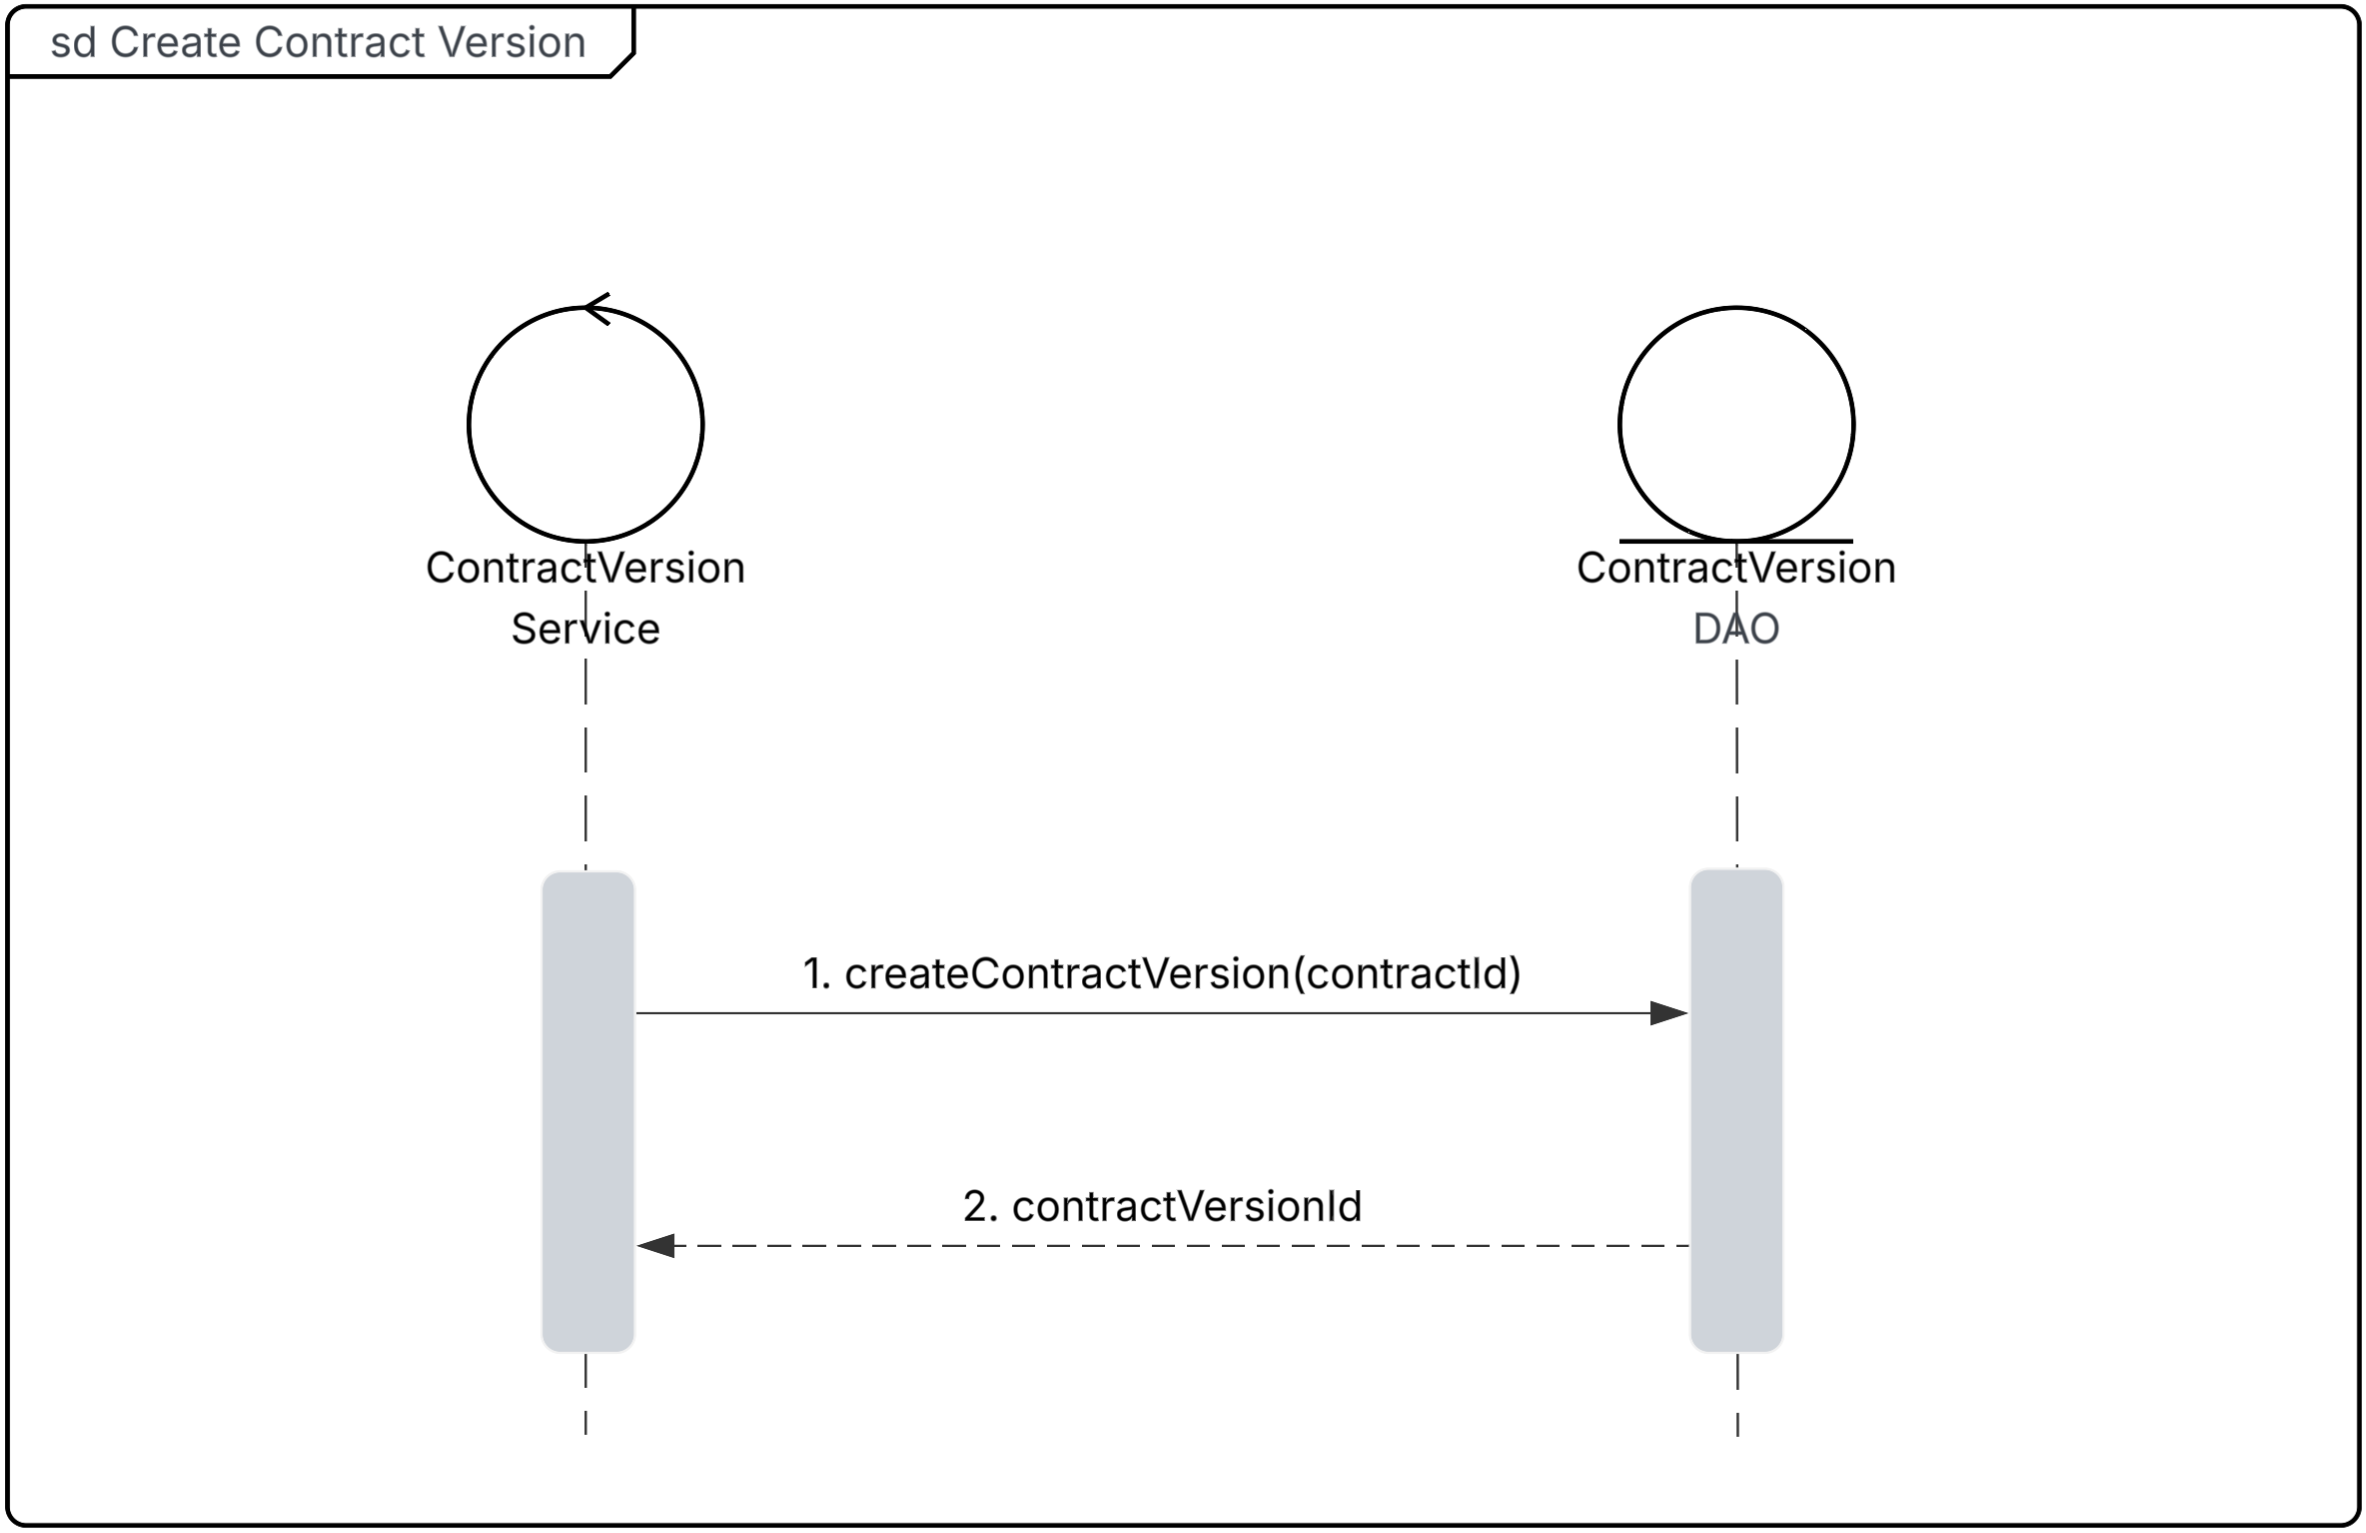
\includegraphics[width=\textwidth]{Images/Sequence Diagram - Create Contract Version Ref.png}
        \captionof{figure}{Sequence Diagram – Create Contract Version}
        \label{fig:sequence_diagram_create_contract_version}
    \end{minipage}

    \vspace{0.5cm}

    \begin{minipage}[t]{0.48\textwidth}
        \centering
        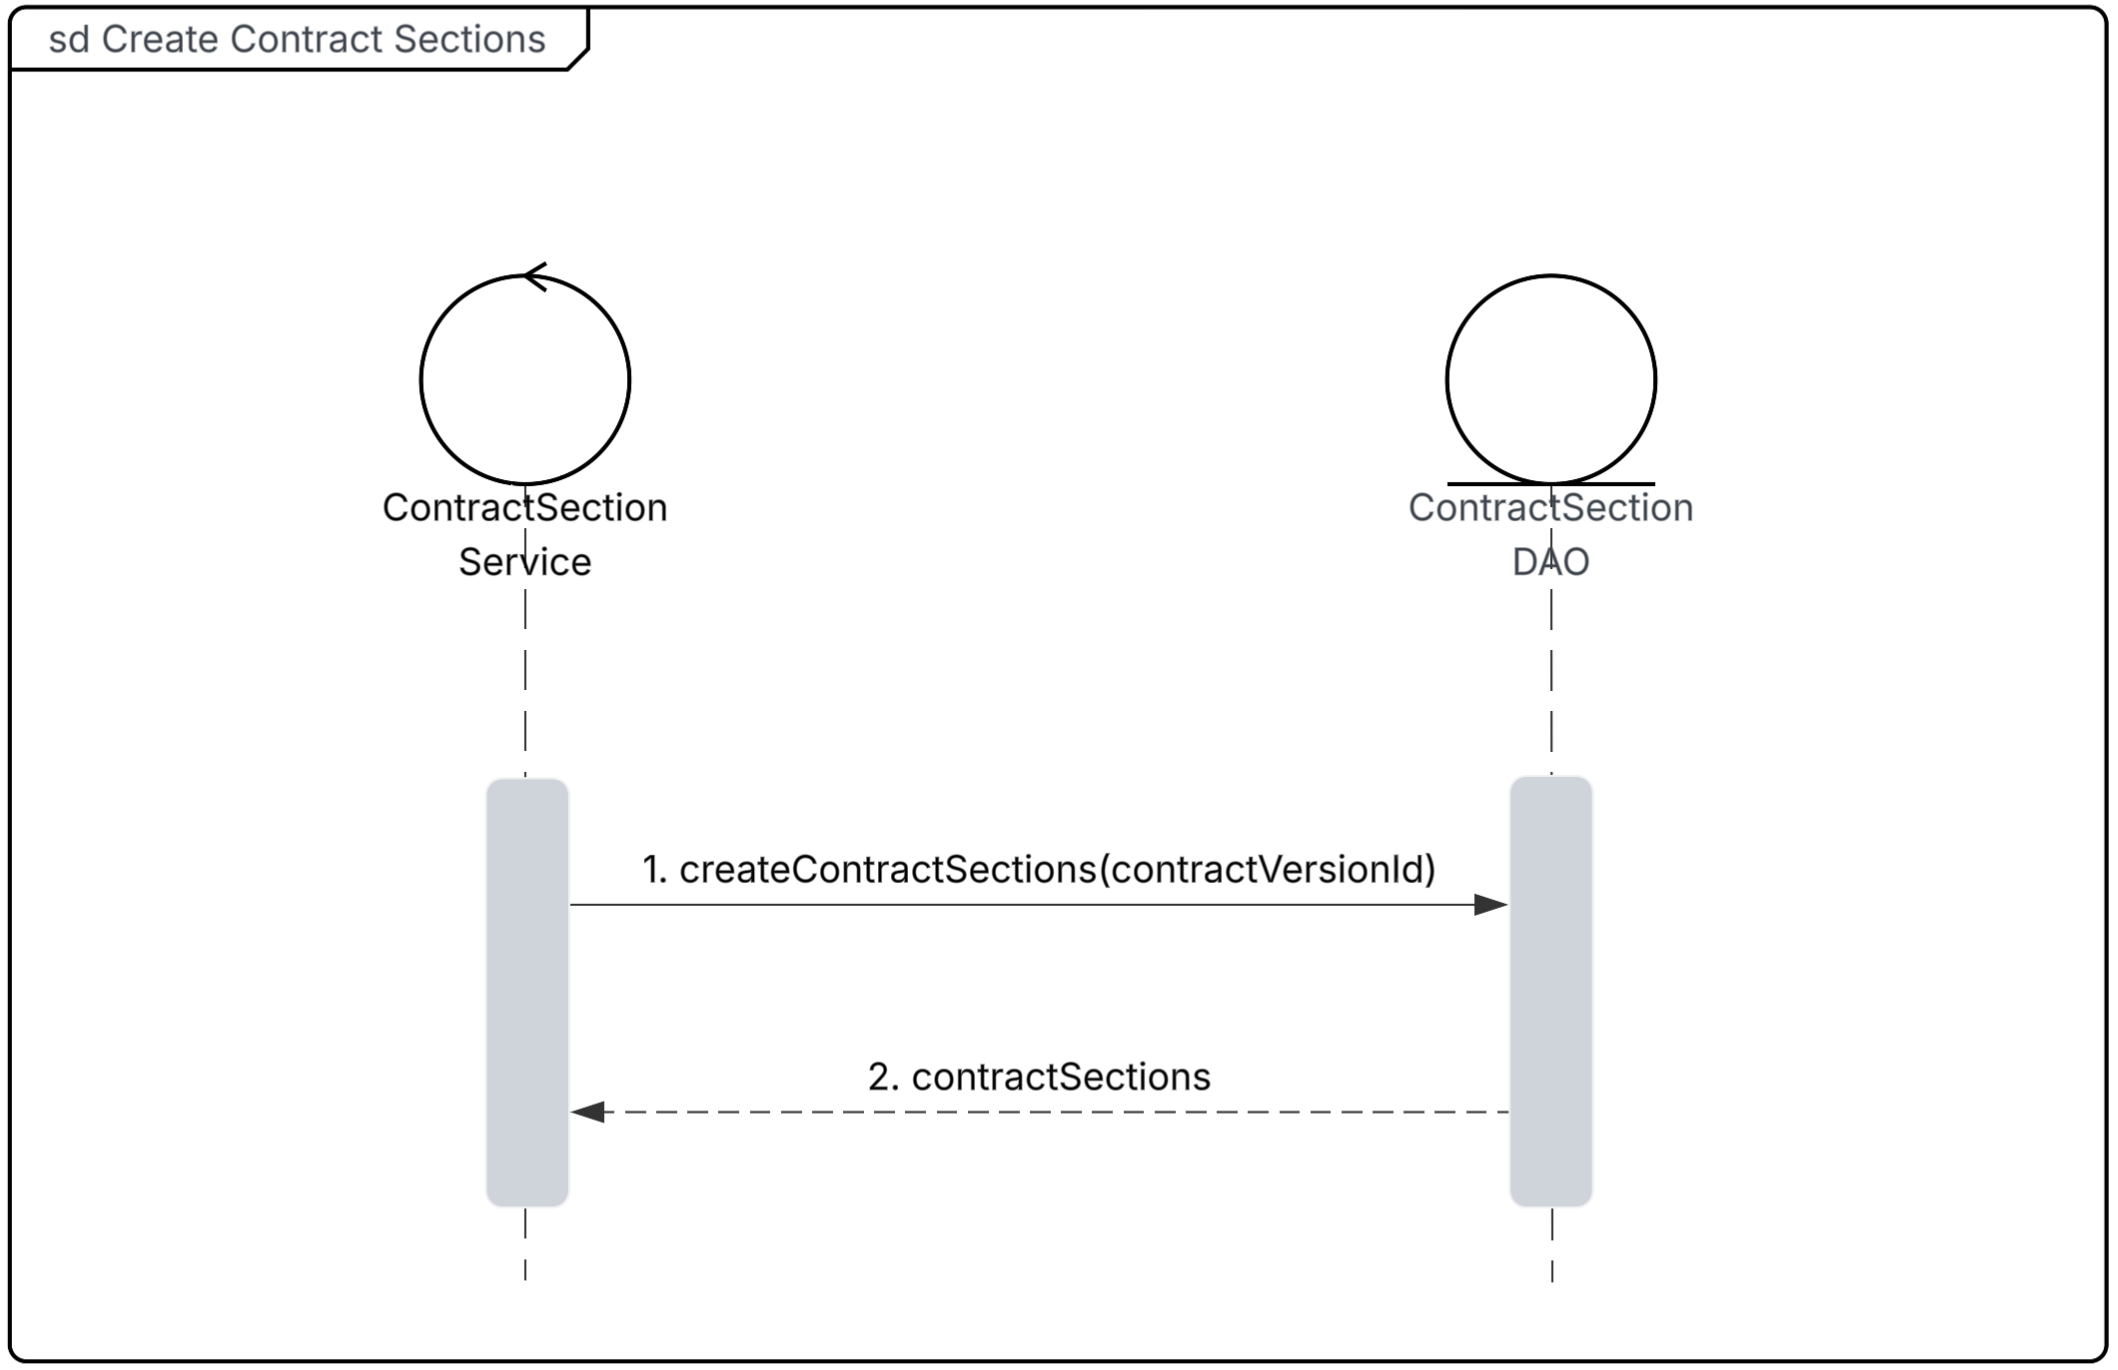
\includegraphics[width=\textwidth]{Images/Sequence Diagram - Create Sections Ref.png}
        \captionof{figure}{Sequence Diagram – Create Contract Sections}
        \label{fig:sequence_diagram_create_sections}
    \end{minipage}
    \hfill
    \begin{minipage}[t]{0.48\textwidth}
        \centering
        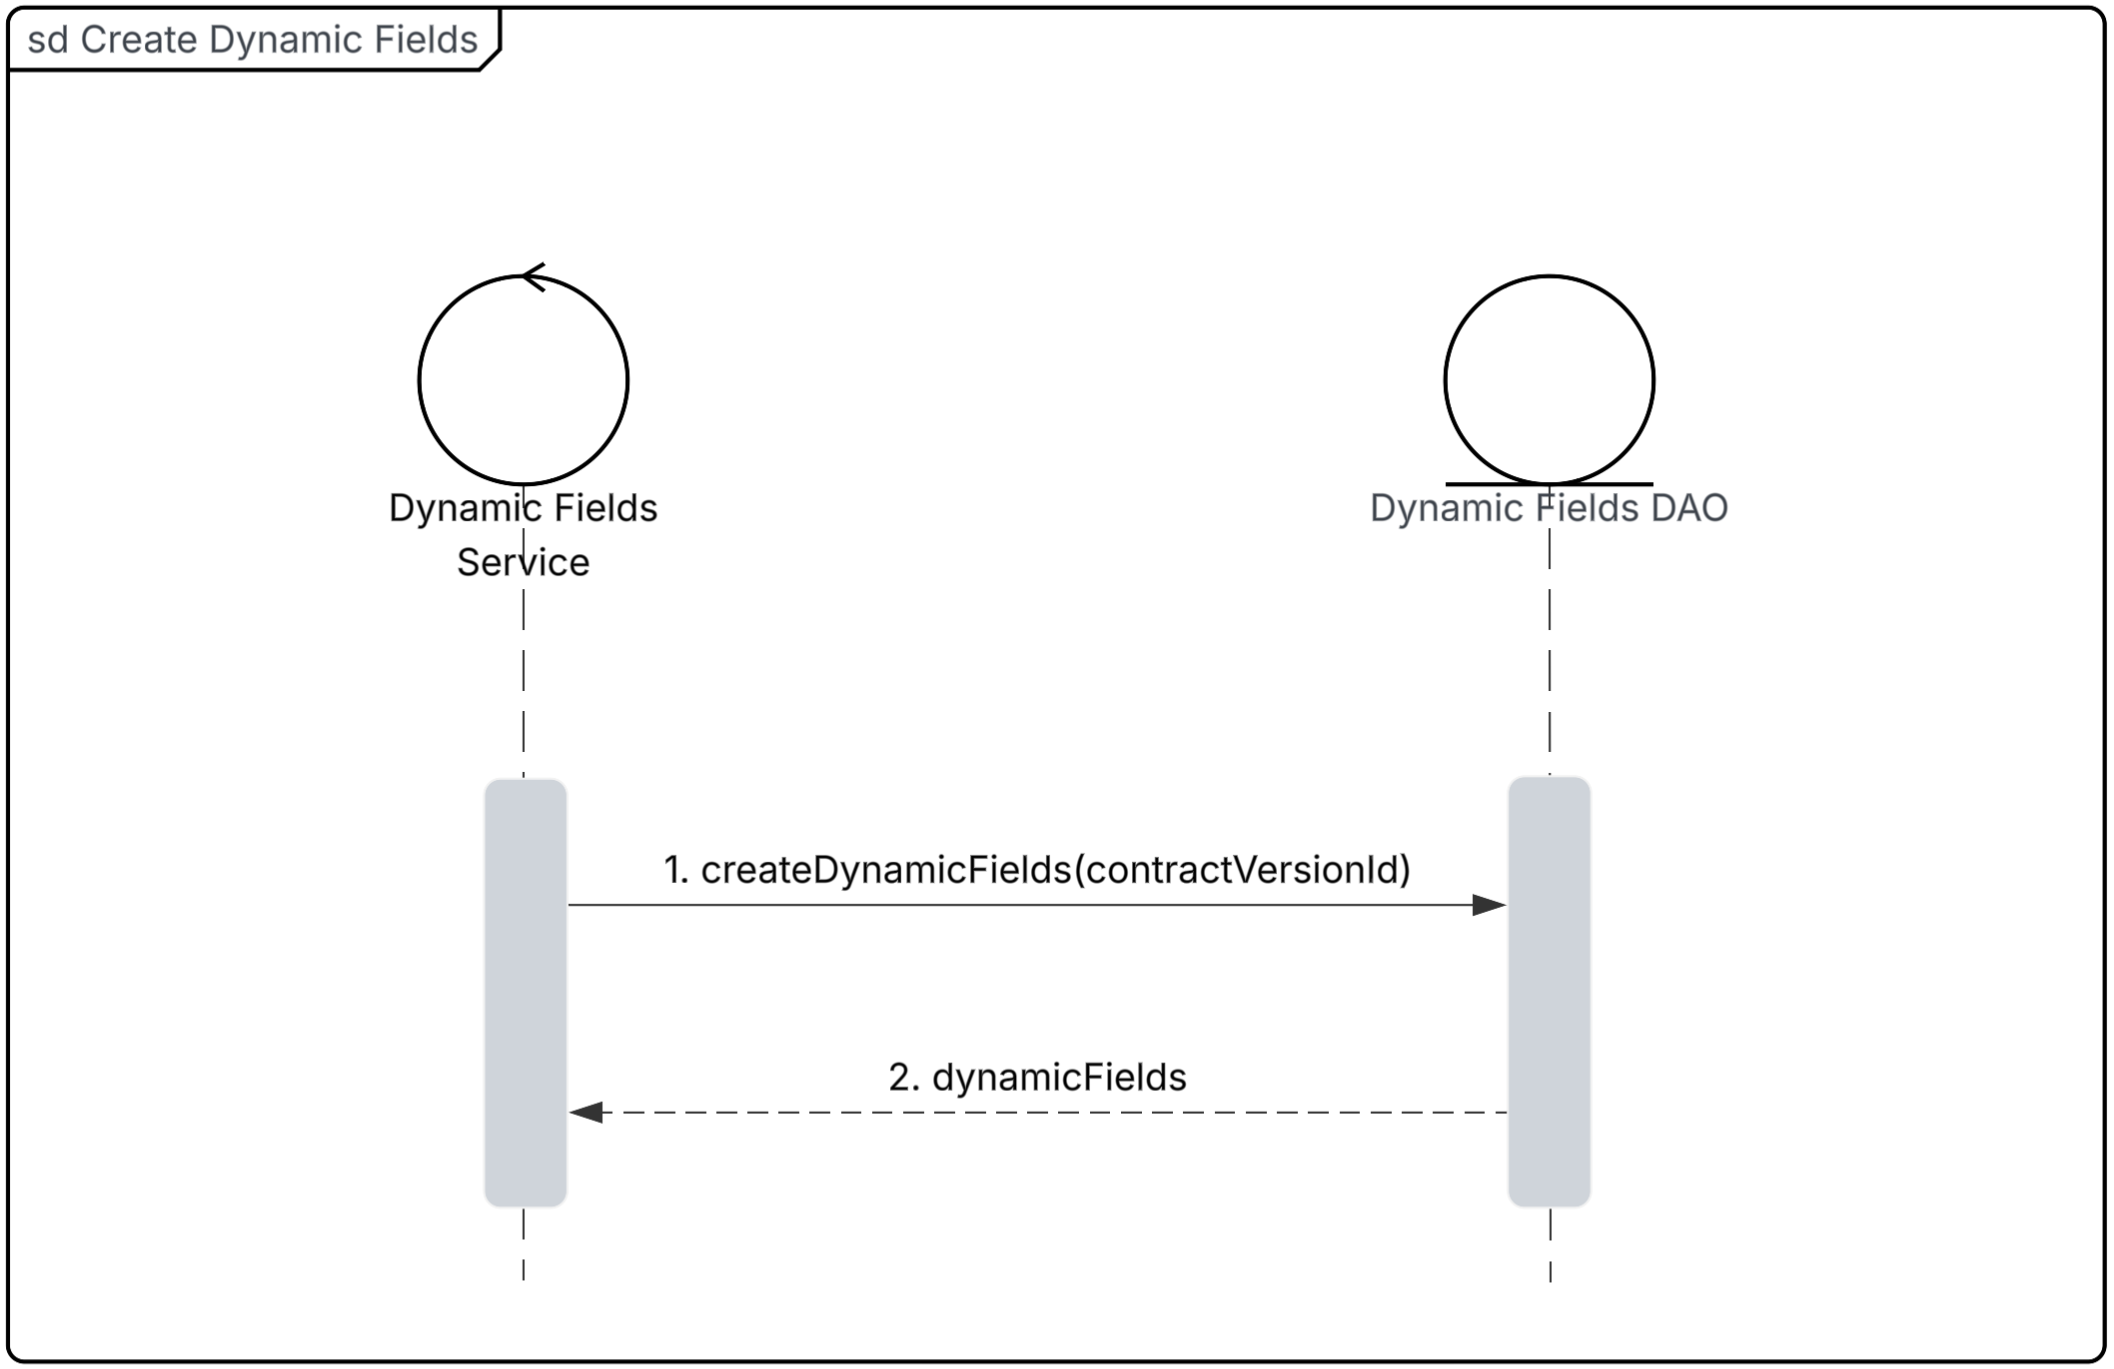
\includegraphics[width=\textwidth]{Images/Sequence Diagram - Create Dynamic Fields Ref.png}
        \captionof{figure}{Sequence Diagram – Create Dynamic Fields}
        \label{fig:sequence_diagram_create_dynamic_fields}
    \end{minipage}

\end{figure}

Figure \ref{fig:sequence_diagram_draft_contract} depicts the detailed sequence diagram for generating a new contract. In this scenario, the sales user initiates by logging into the system and providing a prompt through text, voice, or image, detailing essential information needed for the contract. The system then extracts necessary fields such as Incoterm, contract type, product, and client name to identify the appropriate template and client data. If critical information is missing or a new client is identified, the system prompts the user for clarification or confirmation to avoid mismatches.\mynewline

Upon confirmation, the system creates a new client record if necessary, extracts dynamic fields from the provided prompt, selects the appropriate contract template, and populates the dynamic fields accordingly. Missing fields are filled either by referencing a specific past contract indicated by the user or by defaulting to the client's most recent contract. If the client is new or no relevant contracts are found, fields remain empty. After contract generation, the user is automatically redirected to the contract editing interface.

% Clause Request Lifecycle
\subsubsection{Clause Request Lifecycle}

The Clause Request Lifecycle involves coordinated interactions between sales and legal teams, as shown in Figure \ref{fig:sequence_diagram_clause_request_sales} and Figure \ref{fig:sequence_diagram_clause_request_legal}. Initially, a sales user creates a clause request by providing a description for modifying, adding, or deleting clauses within a contract. The user can optionally refine this description with assistance from the Refiner Agent, which leverages an LLM to enhance clarity and precision. The sales user can then either save the request for later or send it directly to the legal team.\mynewline

Upon submission, the legal team receives a notification of the new clause request. Legal users may reject the request immediately by providing specific feedback or accept it for further processing. Accepted requests prompt legal users to utilize a dedicated editor to craft or modify clauses as requested. Completed clauses may be directly integrated into the active contract by publishing, or saved in the clause library for future use.

\begin{landscape}
\begin{figure}[H]
    \centering
    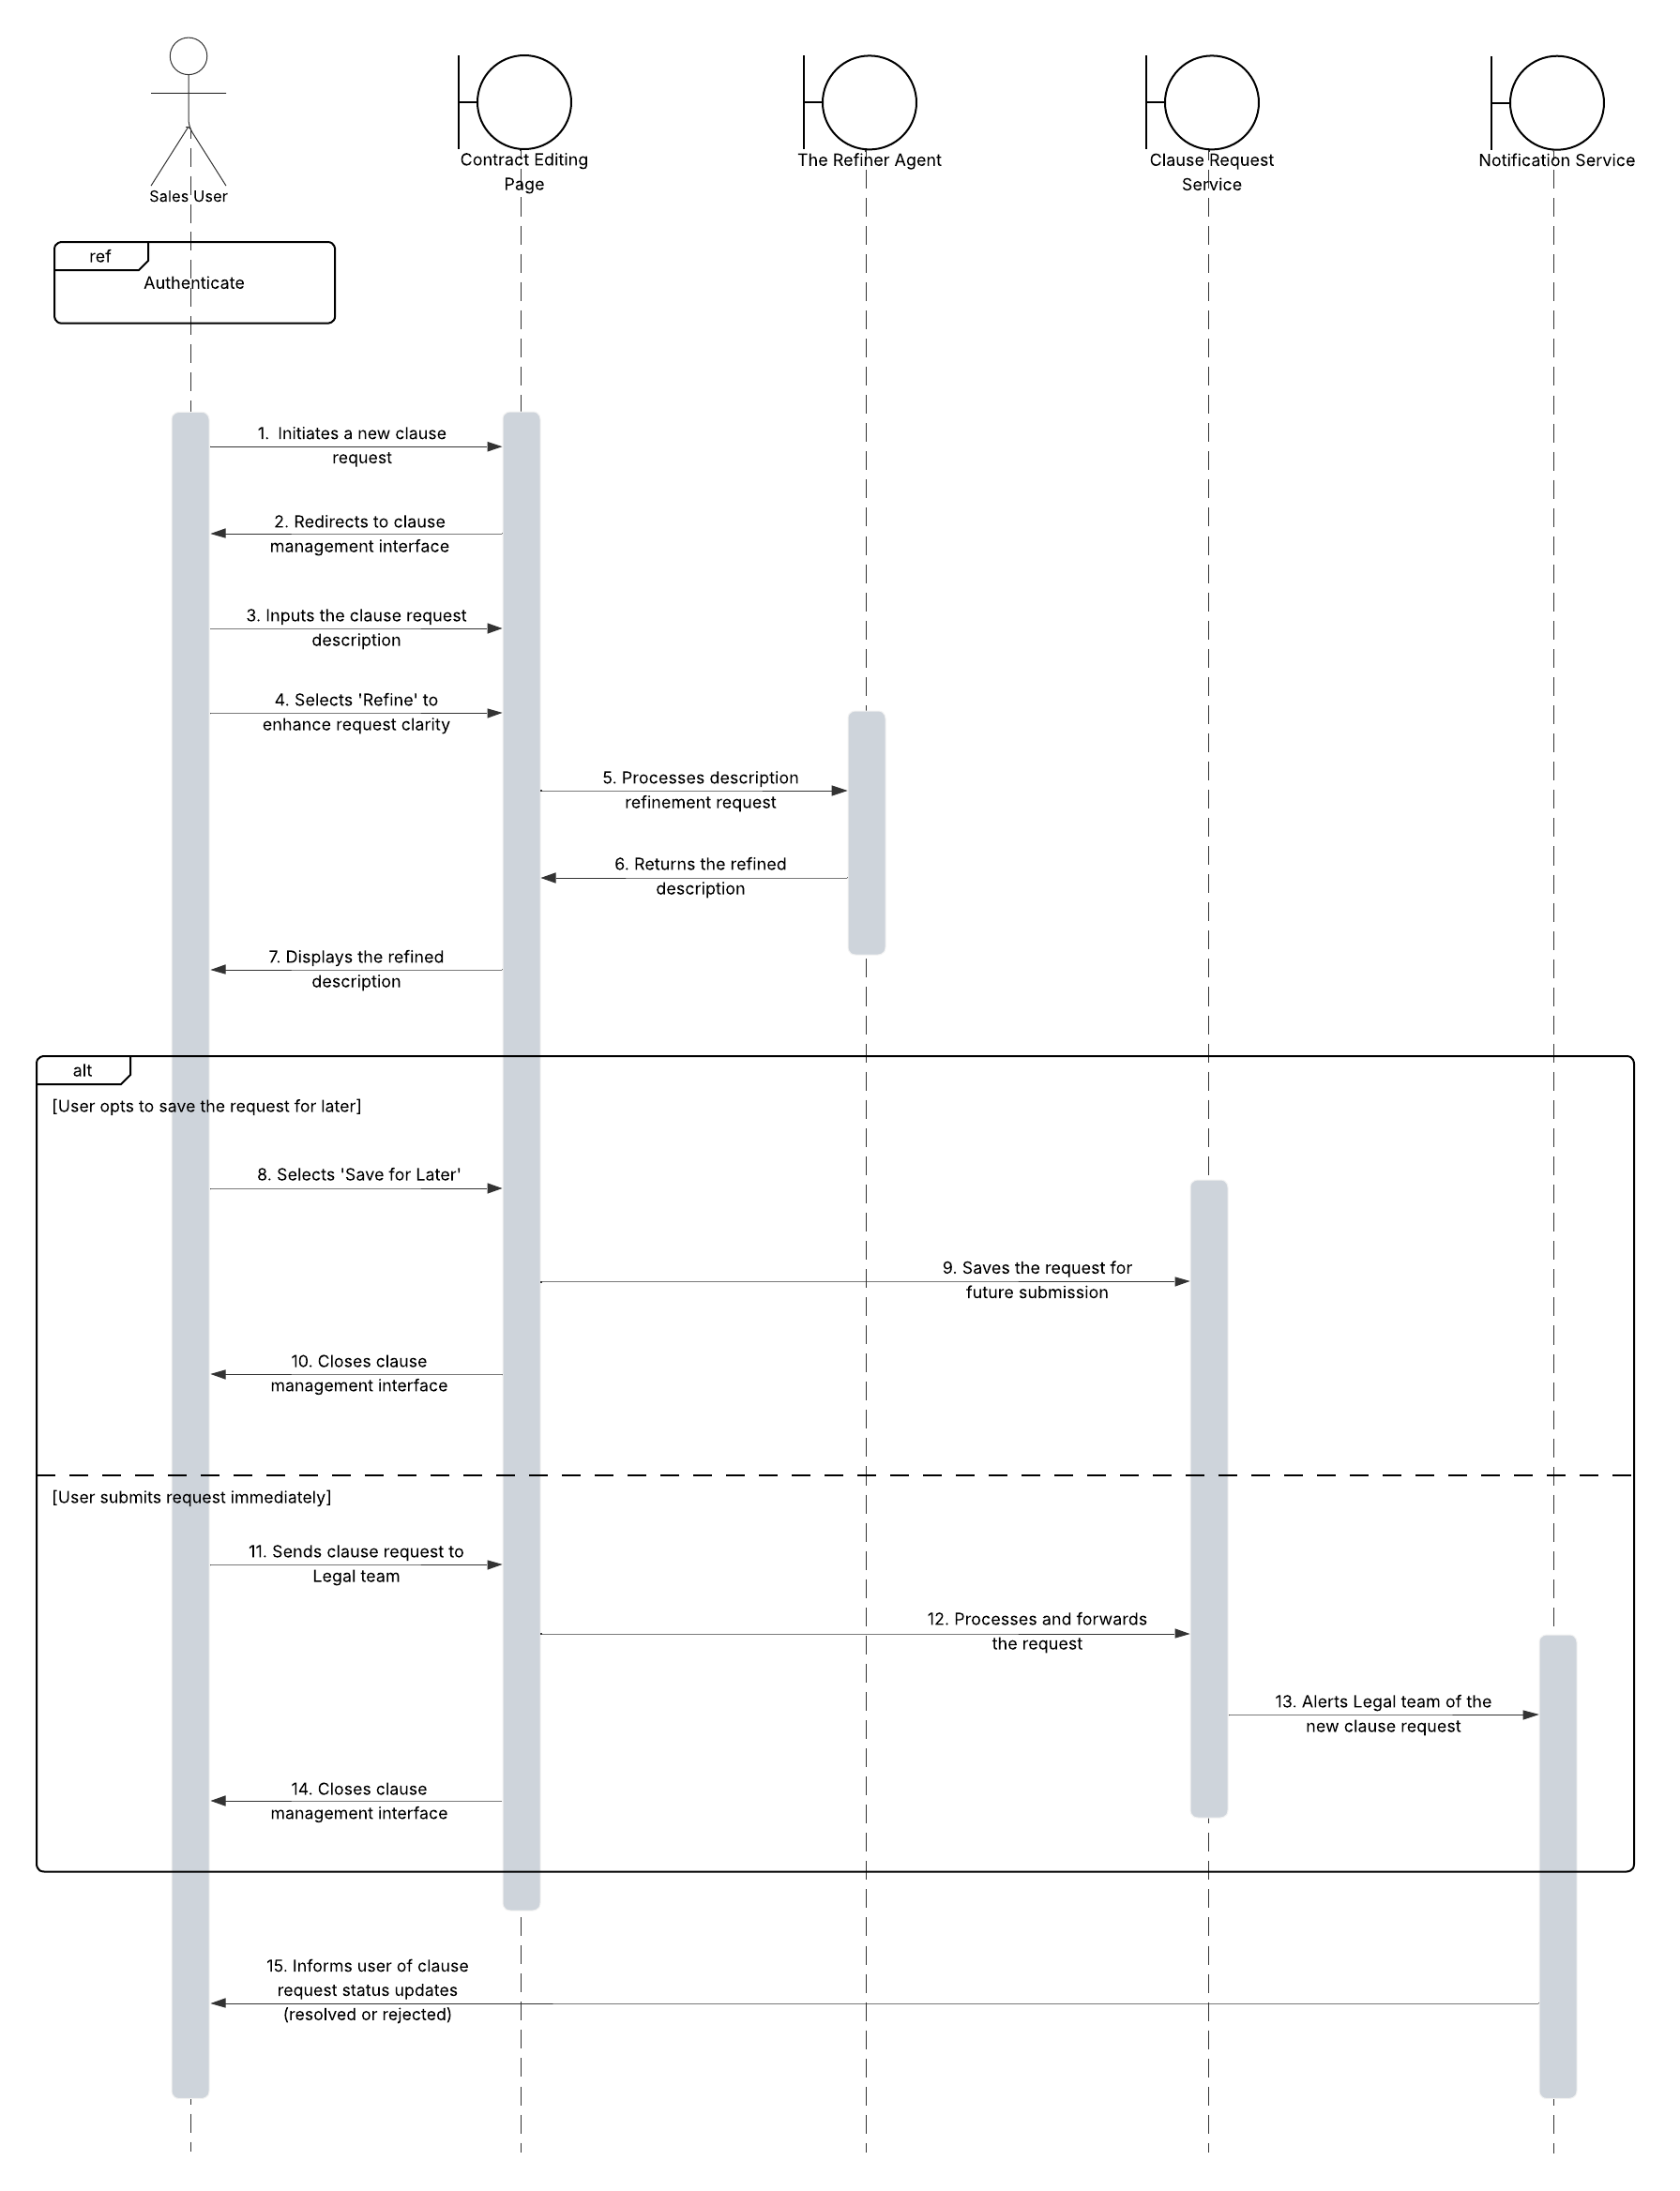
\includegraphics[width=1.1\textwidth]{Images/Sequence Diagram - Sales - Clause Request.png}
    \caption{Sequence Diagram - Clause Request (Sales Perspective)}
    \label{fig:sequence_diagram_clause_request_sales}
\end{figure}
\end{landscape}

\begin{center}
    \centering
    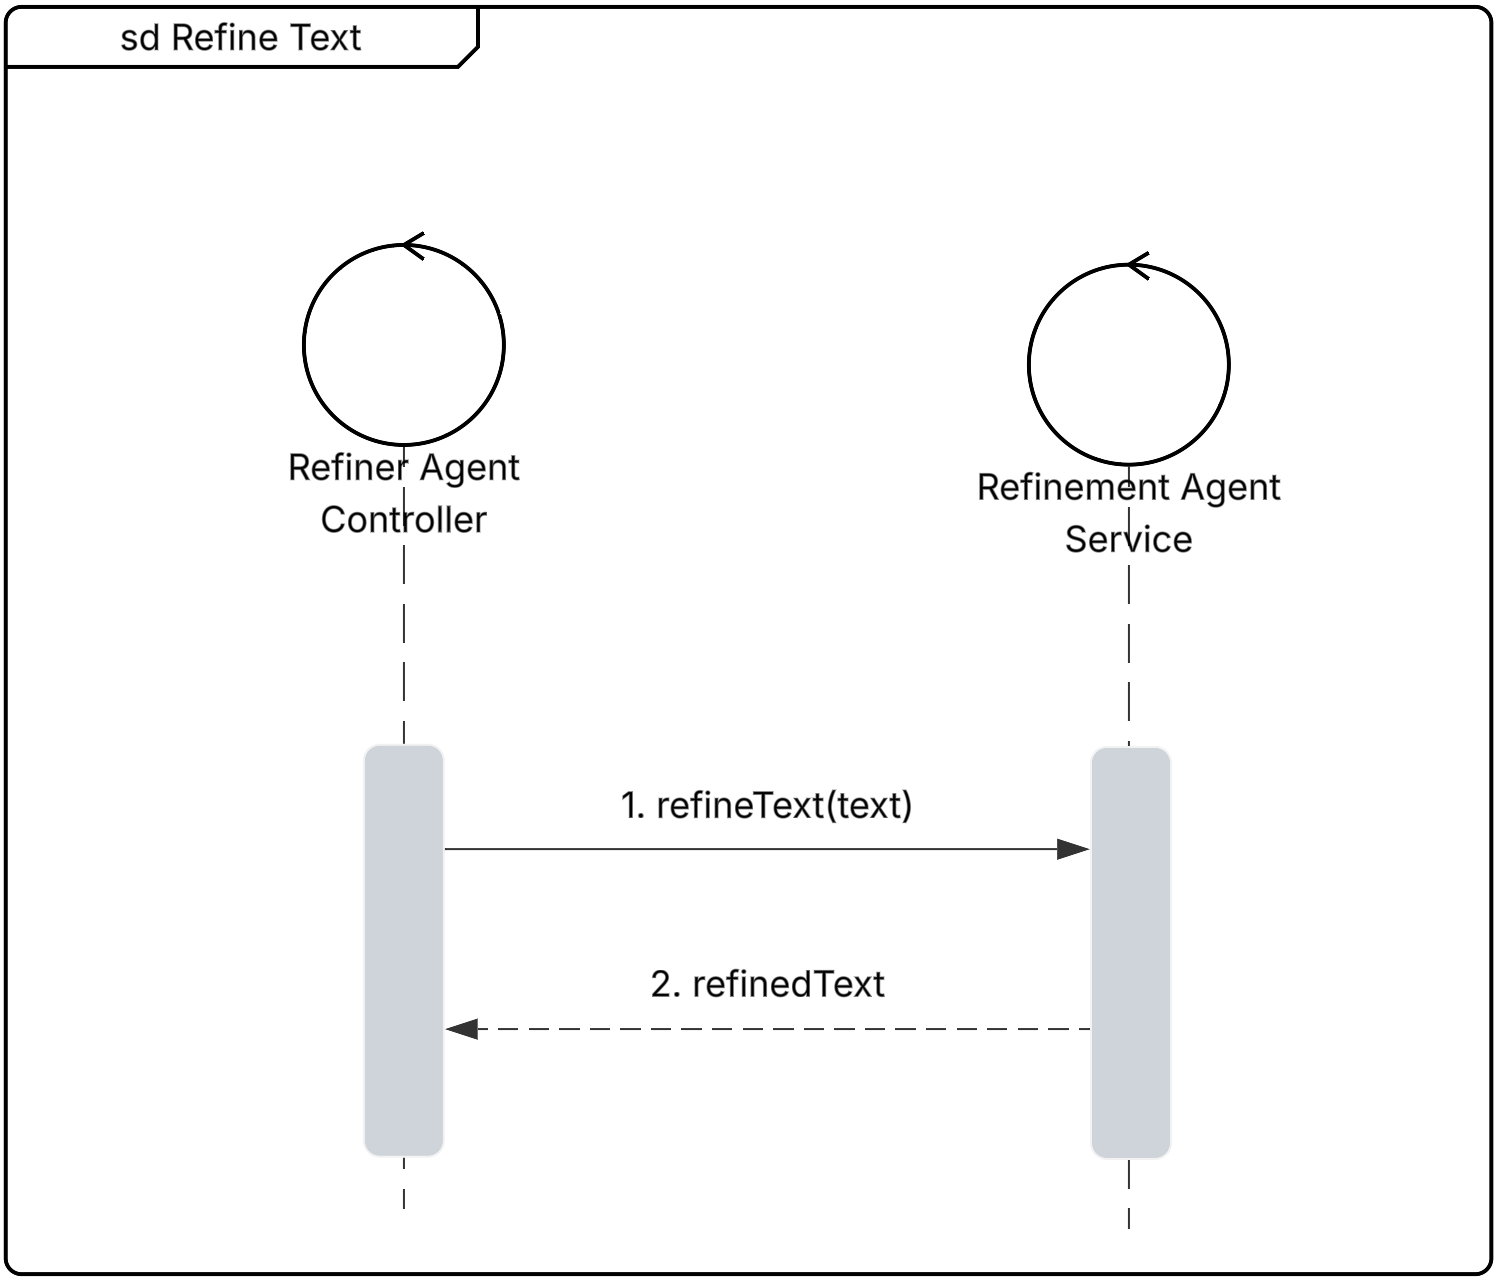
\includegraphics[width=0.48\textwidth]{Images/Sequence Diagram - Refine Text Ref.png}
    \captionof{figure}{Sequence Diagram - Refine Text}
    \label{fig:sequence_diagram_refine_text}
\end{center}

After presenting the clause request process from the Sales user's perspective, the following sequence diagram illustrates the corresponding workflow from the Legal user's point of view:

\begin{landscape}
\begin{figure}[H]
    \centering
    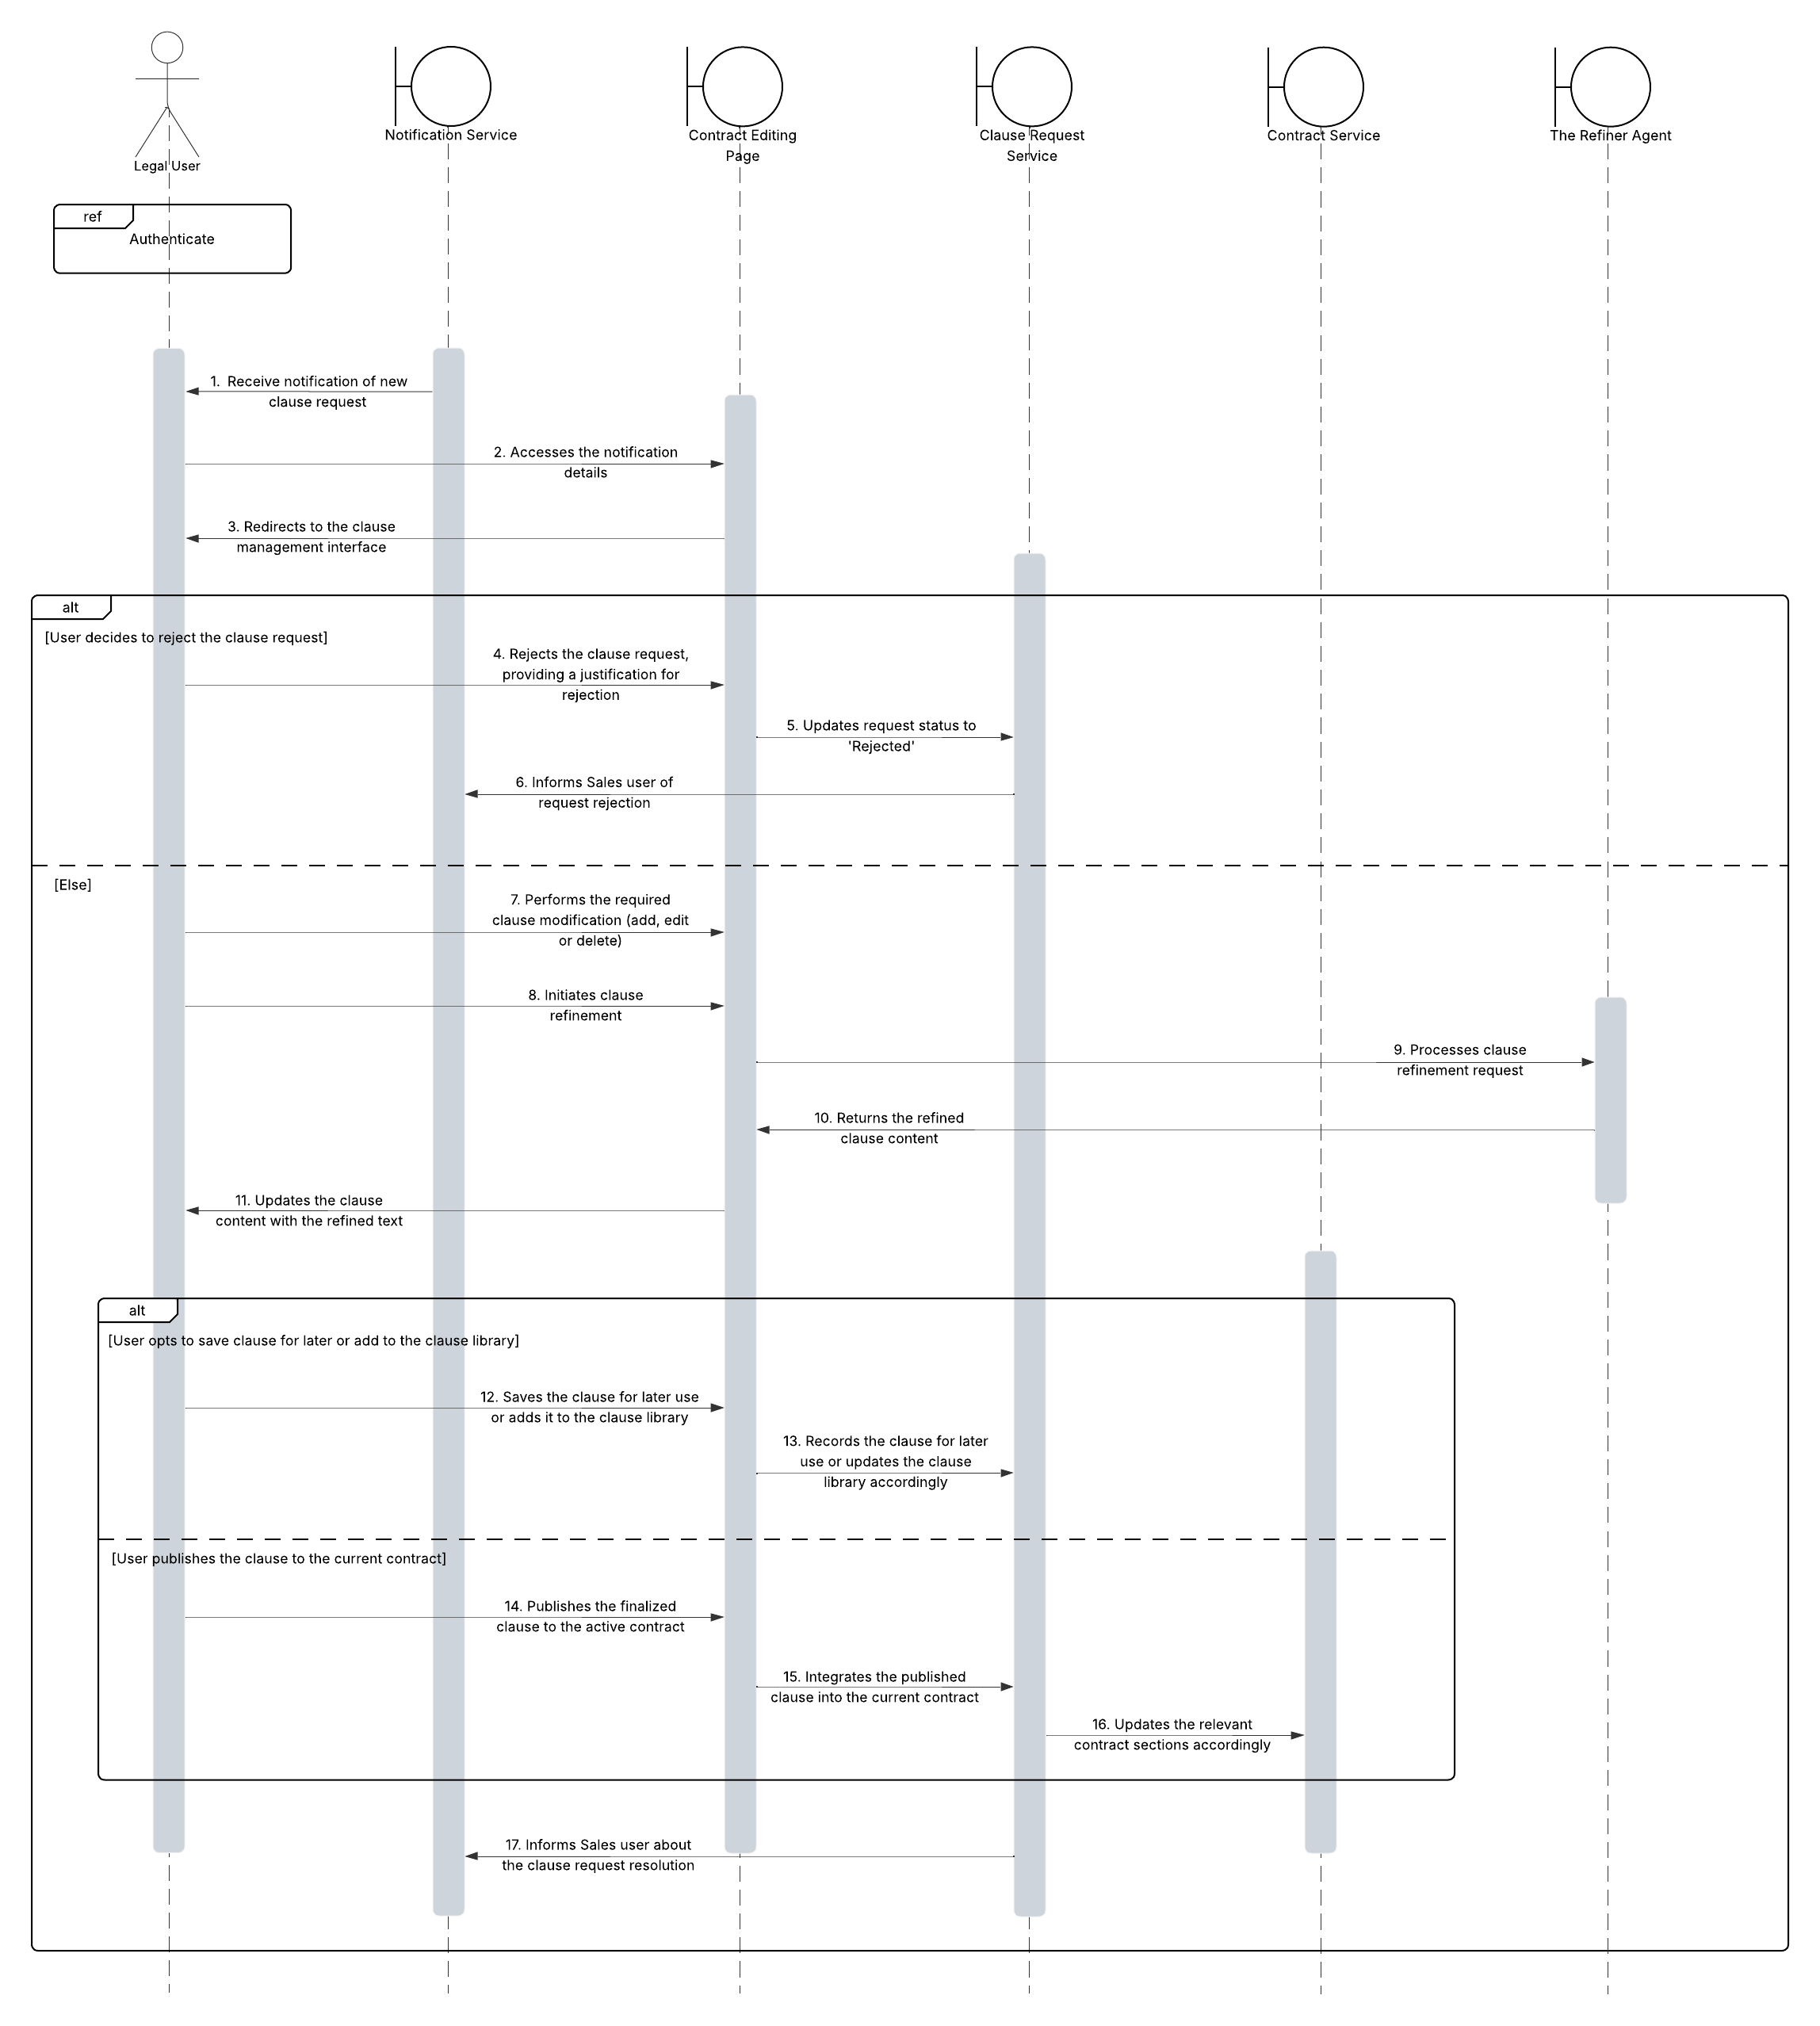
\includegraphics[width=1.3\textwidth]{Images/Sequence Diagram - Legal - Clause Request.png}
    \caption{Sequence Diagram - Clause Request (Legal Perspective)}
    \label{fig:sequence_diagram_clause_request_legal}
\end{figure}
\end{landscape}

\begin{center}
    \centering
    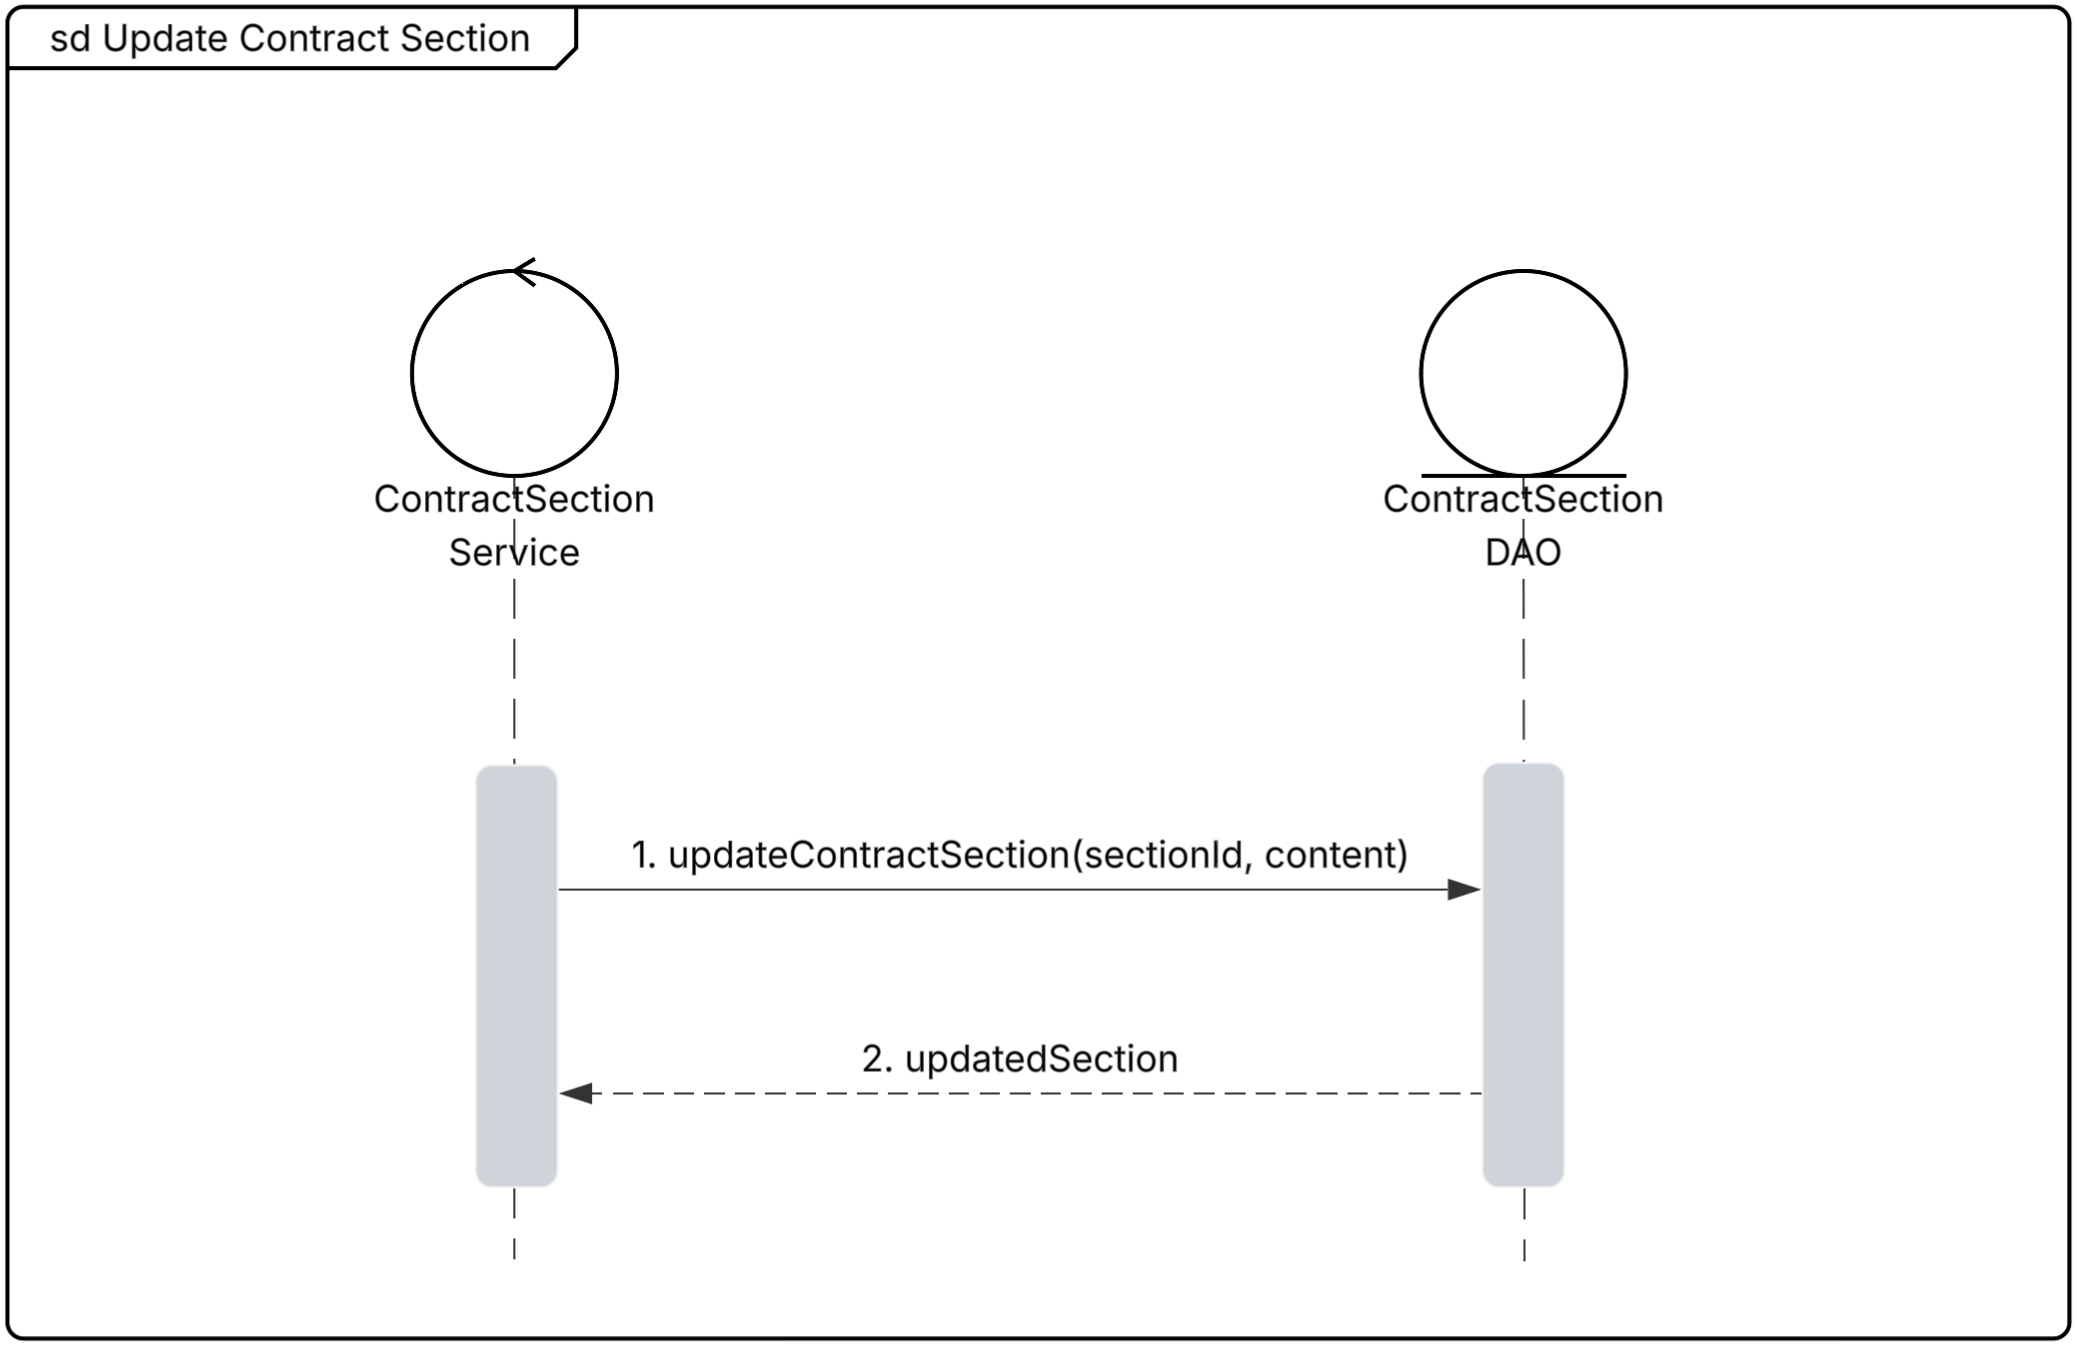
\includegraphics[width=0.48\textwidth]{Images/Sequence Diagram - Update Sections Ref.png}
    \captionof{figure}{Sequence Diagram - Update Contract Sections}
    \label{fig:sequence_diagram_update_contract_sections}
\end{center}

These diagrams comprehensively clarify the interactions between system components, highlighting critical processes and dependencies to ensure a smooth and efficient workflow within the intelligent contract management platform.

% Deployment Architecture
\section{Deployment Architecture}
The deployment architecture is a core operational layer that supports the delivery, testing, and maintenance of the intelligent contract management platform. It enables rapid feature iteration, automated quality control, and consistent deployment across environments. This section outlines how DevOps practices—particularly Continuous Integration and Continuous Deployment (CI/CD)—are integrated into the project’s delivery lifecycle.

\begin{center}
    \centering
    \includegraphics[width=1\textwidth]{Images/Deployment Architecture.png}
    \captionof{figure}{Deployment Architecture Overview}
    \label{fig:deployment_architecture}
\end{center}

The process begins with developers managing tasks via Azure Boards and committing changes to a Git repository. Each push triggers a CI pipeline configured to perform essential validations, including static code analysis using SonarCloud, unit testing, and artifact building. Secrets required during builds are retrieved securely from Azure Key Vault, and integration tests are executed within isolated environments to ensure stability.\mynewline

After successful validation, build artifacts are promoted to the CD pipeline, where IaC (Infrastructure-as-Code) tools such as Terraform and Helm are used to deploy services to Kubernetes clusters across development and production environments. Docker images are stored in Azure Container Registry, enabling versioned and reproducible deployments. These workflows ensure high confidence in new releases and accelerate the delivery of new features while maintaining system reliability and traceability.

% Conclusion
\section{Conclusion}
This chapter presented the platform’s system architecture, from frontend/backend logic to AI integration and legal document editing. It concluded with UML diagrams detailing the software’s structure and component workflows. The next chapter will focus on implementation, key functionalities, and system validation.
\minitoc
\label{Chpt:3}
\clearpage


%%%%%%%%%%%%%%%%%%%%%%%%%%%%%%%%%%%%%
%%%%%   Chapitre 4          %%%%%%%%%
%%%%%%%%%%%%%%%%%%%%%%%%%%%%%%%%%%%%%
\chapter{Implementation and Validation}
This chapter outlines the implementation of the intelligent contract management platform. It starts with a review of the selected technologies across AI, frontend, backend, and infrastructure. The core functionalities—contract drafting, editing, clause handling, and tracking—are described in detail. It also presents the collaborative and review workflows powered by AI agents. Lastly, it explains the validation process for verifying functional and non-functional requirements.

\newpage
\fancyhead[R]{\textsc{Chapter 4 - Implementation}}
\hypertarget{fourthchapter}{}

% Technological Environment
\section{Technological Environment}
The choice of appropriate technologies is critical for ensuring both performance and maintainability. Below, we outline our selected technologies, emphasizing the reasoning behind each choice.

% AI Integration and Workflow Orchestration
\subsection{AI Integration and Workflow Orchestration}

% Azure OpenAI's Large Language Models
\subsubsection{Azure OpenAI's Large Language Models}
Azure OpenAI's Large Language Models (LLMs) were selected for their exceptional performance in generating human-like text and handling complex language tasks. Known for their extensive training on diverse datasets, these models excel in text generation, summarization, and conversational AI, proving essential across multiple application scenarios in our project.\mynewline

The decision to use Azure OpenAI was influenced by specific client requirements, notably the necessity for data security and compliance. The Azure environment allows operations to be confined locally, ensuring sensitive data, particularly legal contracts, remain secure within the client's network. Additionally, opting for Azure OpenAI provided seamless integration with the client's existing infrastructure, including Azure Repos and Azure Pipelines, thus offering an enterprise-grade ecosystem.\mynewline

We concluded that Azure OpenAI's models were the most suitable after considering other alternatives such as Google's BERT and Meta's LLaMA.

\begin{center}
    \centering
    \includegraphics[width=0.2\textwidth]{Images/Azure OpenAI Logo.png}
    \captionof{figure}{Azure OpenAI Logo} \cite{azure_openai_logo}
    \label{fig:azure_openai_logo}
\end{center}

% LangChain
\subsubsection{LangChain}
LangChain was integrated to enable flexible and model-agnostic communication within our system. Its modular nature allows seamless integration with various LLM providers, offering the flexibility to switch models or combine outputs based on specific tasks. This ensures the system remains adaptable to ongoing developments in LLM technology and can readily incorporate future advancements.\mynewline

Additionally, LangChain provides essential utilities for managing conversational flows, context tracking, and connections with external data sources, critical for sophisticated generative AI-driven applications. Its use underpins the modularity and scalability of our architecture, effectively handling complex tasks across diverse domains.\mynewline

LangChain was ultimately selected for its abstraction capabilities after evaluating direct integrations with alternative APIs.

\begin{center}
    \centering
    \includegraphics[width=0.2\textwidth]{Images/LangChain Logo.png}
    \captionof{figure}{LangChain Logo} \cite{langchain_logo}
    \label{fig:langchain_logo}
\end{center}

% LangGraph
\subsubsection{LangGraph}
LangGraph complements LangChain by enabling sophisticated workflow orchestration through a graph-based model. It supports complex, dynamic, and iterative processes within AI workflows, facilitating advanced conditional logic, stateful interactions, and multi-agent collaborations. This capability is especially beneficial for iterative legal document processing tasks, enhancing decision-making capabilities and workflow adaptability.\mynewline

LangGraph was chosen over other orchestration tools for its native compatibility with LangChain and AI-specific use cases.

\begin{center}
    \centering
    \includegraphics[width=0.2\textwidth]{Images/LangGraph Logo.png}
    \captionof{figure}{LangGraph Logo} \cite{langgraph_logo}
    \label{fig:langgraph_logo}
\end{center}

% Vector Databases
\subsection{Vector Databases}
Elasticsearch was selected as the primary vector database due to its exceptional capabilities in managing high-dimensional vector searches, essential for Retrieval-Augmented Generation (RAG) architectures. Elasticsearch facilitates rapid similarity searches, allowing efficient real-time retrieval of relevant documents based on embedding vectors derived from queries. Its scalability, robustness, and comprehensive indexing capabilities were critical in meeting performance expectations under large data volumes while ensuring minimal latency.\mynewline

After comparing it with other solutions like FAISS and Milvus, Elasticsearch was determined to be the most enterprise-ready and integrable option.

\begin{center}
    \centering
    \includegraphics[width=0.2\textwidth]{Images/Elasticsearch Logo.jpg}
    \captionof{figure}{Elasticsearch Logo} \cite{elasticsearch_logo}
    \label{fig:elasticsearch_logo}
\end{center}

% Frontend Technologies and Tooling
\subsection{Frontend Technologies and Tooling}

% Typescript
\subsubsection{TypeScript}
TypeScript is an open-source programming language developed and maintained by Microsoft. It is a strict syntactical superset of JavaScript that adds optional static typing to the language. By enabling developers to define data types for variables, function parameters, and return values, TypeScript improves code clarity, detects potential errors during development, and enhances the scalability of large codebases.\mynewline

TypeScript was adopted for frontend development primarily due to its strong type-checking system, which significantly reduces potential bugs and enhances code maintainability. It compiles directly to JavaScript, enabling native browser execution and optimal performance while retaining compatibility with existing JavaScript libraries and frameworks.\mynewline

We selected TypeScript after evaluating other approaches, concluding it offered the best balance of developer experience, code robustness, and long-term reliability for our frontend needs.

\begin{center}
    \centering
    \includegraphics[width=0.2\textwidth]{Images/TypeScript Logo.png}
    \captionof{figure}{TypeScript Logo} \cite{typescript_logo}
    \label{fig:typescript_logo}
\end{center}

% React
\subsubsection{React}
Developed by Meta (formerly Facebook), React is a popular open-source JavaScript library for building user interfaces, particularly single-page applications. It enables developers to construct interactive UIs using a declarative paradigm and a component-based architecture, where each UI element is encapsulated in a reusable component. Its virtual DOM efficiently updates only the parts of the interface that change, contributing to excellent performance.\mynewline

This modular architecture supports efficient state management and seamless integration with backend services. Combined with React’s widespread community support and flexibility, these features enable the rapid development of dynamic, responsive applications.

\begin{center}
    \centering
    \includegraphics[width=0.2\textwidth]{Images/React Logo.png}
    \captionof{figure}{React Logo} \cite{react_logo}
    \label{fig:react_logo}
\end{center}

% Tiptap
\subsubsection{Tiptap}
Built on top of ProseMirror, Tiptap is a modern, open-source rich-text editor framework designed to be headless and highly extensible. It allows developers to craft custom editing interfaces tailored to specific application needs. Unlike conventional WYSIWYG editors, Tiptap decouples the editing engine from the UI layer, offering full control over document structure, formatting behavior, and content validation—making it ideal for structured documents and domain-specific workflows.\mynewline

Its ability to handle complex legal documents made it a natural fit for our platform. Tiptap supports customized editing experiences, structured clause and variable handling, and real-time collaborative editing. After reviewing alternative editors, its extensibility, legal adaptability, and collaborative compatibility made it the most suitable choice for our use case.

\begin{center}
    \centering
    \includegraphics[width=0.2\textwidth]{Images/TipTap Logo.png}
    \captionof{figure}{TipTap Logo} \cite{tiptap_logo}
    \label{fig:tiptap_logo}
\end{center}

% Testing Libraries
\subsubsection{Testing Libraries}
Developed and maintained by Meta, Jest is a comprehensive JavaScript testing framework primarily designed for React applications, though it also supports a wide range of JavaScript and TypeScript projects. It comes equipped with powerful features such as test runners, assertions, mocking capabilities, code coverage analysis, and snapshot testing. Its zero-configuration setup and intuitive syntax make it accessible to developers of all experience levels.\mynewline

Thanks to its efficiency, ease of configuration, and robust mocking tools, Jest proved ideal for unit and integration testing within our TypeScript and React stack. Among several alternatives, it stood out for its mature ecosystem, fast performance, and seamless integration with modern frontend tooling.

\begin{center}
    \centering
    \includegraphics[width=0.2\textwidth]{Images/Jest Logo.png}
    \captionof{figure}{Jest Logo} \cite{jest_logo}
    \label{fig:jest_logo}
\end{center}

% Backend Technologies and Tooling
\subsection{Backend Technologies and Tooling}

% Python
\subsubsection{Python}
Python is a high-level, interpreted programming language renowned for its simplicity, readability, and versatility. It supports multiple programming paradigms, including procedural, object-oriented, and functional programming. Python has a rich ecosystem of libraries and frameworks, particularly in the fields of web development, data analysis, and artificial intelligence, making it one of the most widely used languages in both academia and industry.\mynewline

Its extensive support for machine learning and natural language processing—most notably through libraries like LangChain—made Python the preferred backend language for our project. Its clean syntax and strong community support enabled rapid development, easy maintenance, and seamless AI integration. After evaluating multiple options, Python’s unmatched flexibility and robust ecosystem positioned it as the most suitable choice for our needs.

\begin{center}
    \centering
    \includegraphics[width=0.2\textwidth]{Images/Python Logo.png}
    \captionof{figure}{Python Logo} \cite{python_logo}
    \label{fig:python_logo}
\end{center}

% FastAPI
\subsubsection{FastAPI}
FastAPI is a modern, high-performance web framework for building APIs with Python 3.7+, leveraging standard type hints and asynchronous programming via async and await. This enables non-blocking I/O operations and supports highly concurrent API services. One of its standout features is the automatic generation of interactive OpenAPI documentation, making it highly developer-friendly and ideal for rapidly building and testing RESTful services.\mynewline

Its performance, simplicity, and native async support made FastAPI an excellent fit for developing high-throughput APIs. Combined with robust type validation via Pydantic, the framework promotes clean, maintainable code. After evaluating multiple frameworks, it emerged as the most effective solution for building fast and reliable APIs in Python.

\begin{center}
    \centering
    \includegraphics[width=0.2\textwidth]{Images/FastAPI Logo.jpg}
    \captionof{figure}{FastAPI Logo} \cite{fastapi_logo}
    \label{fig:fastapi_logo}
\end{center}

% Testing Libraries
\subsubsection{Testing Libraries}
Pytest is a feature-rich testing framework for Python that supports everything from simple unit tests to complex functional and integration scenarios. It prioritizes readability and scalability, offering fixtures, parameterized tests, and assert rewriting. Its plugin-based architecture and support for parallel test execution make it ideal for testing large and sophisticated codebases.\mynewline

We adopted Pytest for backend testing due to its concise syntax, versatility, and robust plugin ecosystem. Among various Python testing tools, it proved to be the most extensible and efficient choice, streamlining our workflow for validating the platform’s core services.

\begin{center}
    \centering
    \includegraphics[width=0.2\textwidth]{Images/Pytest Logo.png}
    \captionof{figure}{Pytest Logo} \cite{pytest_logo}
    \label{fig:pytest_logo}
\end{center}

% SQL Databases
\subsection{SQL Databases}
Given the platform's need for transactional consistency, relational data integrity, and advanced query support, an SQL-based approach was favored over NoSQL. SQL databases better accommodate structured data, complex relationships, and reporting use cases relevant to our application.\mynewline

PostgreSQL was chosen for its advanced query capabilities, robust support for both structured and unstructured data, high performance, extensibility, and strict adherence to ACID transactions. These attributes were critical for efficiently managing the hybrid data requirements inherent in our GenAI-powered system.\mynewline

Among various relational databases, PostgreSQL was selected as the most capable and scalable option for our backend architecture.

\begin{center}
    \centering
    \includegraphics[width=0.2\textwidth]{Images/PostgreSQL Logo.png}
    \captionof{figure}{PostgreSQL Logo} \cite{postgresql_logo}
    \label{fig:postgresql_logo}
\end{center}

% API Testing
\subsection{API Testing}

% Postman
\subsubsection{Postman}
As a comprehensive API platform, Postman simplifies the creation, testing, and documentation of APIs through its intuitive interface. Within our project, it played a key role in verifying API functionality by streamlining request validation and response analysis. Its robust testing capabilities—including automated testing and request chaining—enabled thorough validation of API behavior.\mynewline

We selected Postman as our primary API testing tool for its ease of use, extensive features, and superior usability compared to other evaluated options.

\begin{center}
    \centering
    \includegraphics[width=0.2\textwidth]{Images/Postman Logo.png}
    \captionof{figure}{Postman Logo} \cite{postman_logo}
    \label{fig:postman_logo}
\end{center}

% cURL
\subsubsection{cURL}
cURL stands us a lightweight yet powerful command-line tool for API testing, offering a way to interact with APIs directly from the terminal. In our project, cURL serves as a solution for quick and efficient API testing, providing control over HTTP requests and responses. While lacking the graphical interface of tools like Postman, cURL compensates with its simplicity and speed.\mynewline

Due to its flexibility and universal compatibility, cURL complemented our testing stack effectively.

\begin{center}
    \centering
    \includegraphics[width=0.2\textwidth]{Images/cURL Logo.png}
    \captionof{figure}{cURL Logo} \cite{curl_logo}
    \label{fig:curl_logo}
\end{center}

% Static Code Analysis and Quality Assurance
\subsection{Static Code Analysis and Quality Assurance}
SonarQube is a static code analysis tool designed to detect bugs, identify security vulnerabilities, and evaluate source code quality. In this project, SonarQube was employed to analyze both existing code and newly developed features. The tool facilitated the correction of detected bugs and security flaws, offering actionable recommendations to enhance code structure and readability, thus ensuring compliance with the client's quality standards.\mynewline

SonarQube was selected after comparing several tools, as it offered the best combination of analysis depth, usability, and integration capabilities.

\begin{center}
    \centering
    \includegraphics[width=0.2\textwidth]{Images/SonarQube Logo.png}
    \captionof{figure}{SonarQube Logo} \cite{sonarqube_logo}
    \label{fig:sonarqube_logo}
\end{center}

% CI/CD Pipelines
\subsection{CI/CD Pipelines}
Azure Pipelines, part of the Microsoft Azure DevOps suite, is a cloud-based CI/CD service that automates the building, testing, and deployment of code across diverse platforms and environments. It integrates seamlessly with popular source control systems and cloud services, offering powerful automation and precise control over deployment workflows.\mynewline

In our project, Azure Pipelines—along with Azure Repos—was used to streamline continuous integration and deployment processes. This choice aligned with the client’s infrastructure, enabling seamless integration, robust version control, and efficient automation. Its native compatibility with the Azure ecosystem made it the optimal solution for our CI/CD and DevOps needs.

\begin{center}
    \centering
    \includegraphics[width=0.2\textwidth]{Images/Azure Pipelines Logo.jpg}
    \captionof{figure}{Azure Pipelines Logo} \cite{azure_pipelines_logo}
    \label{fig:azure_pipelines_logo}
\end{center}

% Containerization and Orchestration
\subsection{Containerization and Orchestration}

% Docker
\subsubsection{Docker}
As an open-source platform, Docker automates the deployment of applications as portable, self-sufficient containers by packaging code, libraries, and dependencies into isolated units that run reliably across various environments. It streamlines the development lifecycle by ensuring consistent environments from development to production and integrates seamlessly with orchestration tools and cloud platforms.\mynewline

We selected Docker to containerize applications and their dependencies, ensuring reliability across all stages. Although Podman was considered for its rootless architecture, Docker’s widespread adoption, mature ecosystem, and ease of use made it the preferred choice for our project.

\begin{center}
    \centering
    \includegraphics[width=0.2\textwidth]{Images/Docker Logo.png}
    \captionof{figure}{Docker Logo} \cite{docker_logo}
    \label{fig:docker_logo}
\end{center}

% Kubernetes
\subsubsection{Kubernetes}
Originally developed by Google and now maintained by the Cloud Native Computing Foundation (CNCF), Kubernetes is an open-source platform for orchestrating containerized applications. It automates deployment, scaling, and management, offering advanced features like service discovery, load balancing, self-healing, and automated rollouts.\mynewline

Its robust ecosystem and enterprise-grade capabilities made Kubernetes the top choice for orchestration. While alternatives such as Docker Swarm and Apache Mesos were reviewed, Kubernetes stood out as the most powerful and production-ready solution for our deployment needs.

\begin{center}
    \centering
    \includegraphics[width=0.2\textwidth]{Images/Kubernetes Logo.png}
    \captionof{figure}{Kubernetes Logo} \cite{kubernetes_logo}
    \label{fig:kubernetes_logo}
\end{center}

% Terraform
\subsubsection{Terraform}
Developed by HashiCorp, Terraform is an open-source infrastructure as code (IaC) tool that enables users to define and provision both cloud and on-premises infrastructure using a declarative configuration language (HCL). With support for multiple cloud providers and a strong provider ecosystem, Terraform maintains infrastructure state and ensures safe, efficient changes.\mynewline

Its flexibility, cloud-agnostic nature, and version control support made Terraform the ideal tool for managing our infrastructure. After comparing it with AWS CloudFormation and Ansible, we concluded that its multi-cloud capabilities and extensibility made it the optimal solution for our IaC strategy.

\begin{center}
    \centering
    \includegraphics[width=0.2\textwidth]{Images/Terraform Logo.png}
    \captionof{figure}{Terraform Logo} \cite{terraform_logo}
    \label{fig:terraform_logo}
\end{center}

% IDE (Integrated Development Environment)
\subsection{IDE (Integrated Development Environment)}
Visual Studio Code (VS Code) is a an IDE (Integrated Development Environment) with powerful developer tooling like code editing, debugging, version control integration, and support for various programming languages and frameworks. Its user-friendly interface and intuitive design streamline the coding process, allowing us to write and edit code with ease. Additionally, VS Code offers robust Docker integration, enabling us to manage containers and write YAML files for Kubernetes, simplifying our local deployment and testing workflows.\mynewline

VS Code was chosen due to its lightweight design, extensive extension ecosystem, and strong support for containerized development workflows.

\begin{center}
    \centering
    \includegraphics[width=0.2\textwidth]{Images/VS Code Logo.png}
    \captionof{figure}{VS Code Logo} \cite{vscode_logo}
    \label{fig:vscode_logo}
\end{center}

% Implementation
\section{Implementation}
This section is dedicated to presenting the implementation details of the developed solution. Specifically, we outline the interfaces related to contract management functionalities, including contract repository, contract creation, editing, review, notification handling, and history management. The implementation and interfaces associated with other modules were allocated to and handled by different members of the project team, thus falling outside the scope of this section.

% Contract Repository
\subsection{Contract Repository}

The Contract Repository interface is accessible by both Sales and Legal users, serving as the primary dashboard displaying a list of existing client contracts. Contracts are categorized into three distinct statuses: \textbf{In Editing} (editable by both Sales and Legal teams), \textbf{In Review} (finalized by Sales and awaiting Legal review), and \textbf{Finalized} (reviewed, approved, and ready for client delivery).

Each contract card provides essential details, including the title, client involved, contract type, and Incoterms, and supports specific actions such as:

\begin{itemize}
    \item \textbf{Archive/Delete}: Exclusive to Sales users, this functionality enables users to either \textit{delete} a contract completely from the system, primarily used for erroneous entries, or \textit{archive} contracts, which removes them from the main repository interface but retains them in an archived section for future reference or audits.
    \item \textbf{Logs/Notifications}: Users receive relevant notifications reflecting significant changes, such as contract status updates, ensuring stakeholders remain consistently informed and engaged.
\end{itemize}

\begin{center}
    \centering
    \includegraphics[width=1\textwidth]{Images/Contract Repository Page.png}
    \captionof{figure}{Contract Repository Interface}
    \label{fig:contract_repository_page}
\end{center}

% Contract Generation
\subsection{Contract Generation}
From the Contract Repository page, Sales users initiate contract creation via three input methods: audio recording, image uploads, or textual prompts. For instance, a user might prompt: \textit{\"Draft a spot contract for rock product with Incoterm CFR for new client theClientName\"}, optionally supplemented with additional image-based information.

\begin{center}
    \centering
    \includegraphics[width=1\textwidth]{Images/Generate Contract Component.png}
    \captionof{figure}{Contract Creation Component}
    \label{fig:contract_creation_component}
\end{center}

The first agent involved is the Generator, which initially checks for the required information: Contract Type, Incoterm, Client, and Product. Each combination of these fields corresponds to a distinct contract template. In the current scenario, the Generator detects that all essential fields are provided but identifies \textbf{theClientName} as a new client, not yet registered in the database. Consequently, the user is prompted either to confirm the new client details to avoid potential mismatches or, if the client already exists, to utilize an input field that suggests similar existing client names through Elasticsearch-based logic for selecting the correct one.

\begin{center}
    \centering
    \includegraphics[width=1\textwidth]{Images/Generation Contract - Checking Required Fields.png}
    \captionof{figure}{Contract Verifying Fields Step}
    \label{fig:contract_verifying_fields_step}
\end{center}

The contract generation process involves the Generator agent, performing several key steps:

\begin{itemize}
    \item \textbf{Checking}: Confirms necessary fields (Contract Type, Incoterm, Client, Product) are provided. For new clients, users confirm client details or select from suggested matches using Elasticsearch.
    \item \textbf{Generating}: Creates contract sections and dynamically fills fields, leveraging historical data for existing clients to suggest relevant articles.
    \item \textbf{Filling}: Populates contract fields into respective database tables (Contracts, Contract Fields, Versions), and generates the initial contract version.
\end{itemize}

\begin{center}
    \centering
    \includegraphics[width=1\textwidth]{Images/Generation Contract - Steps.png}
    \captionof{figure}{Contract Generating Process}
    \label{fig:contract_generation_steps}
\end{center}

% Contract Editor
\subsection{Contract Editor}
\begin{center}
    \centering
    \includegraphics[width=1\textwidth]{Images/Contract Editor Page.png}
    \captionof{figure}{Contract Editor Interface}
    \label{fig:contract_editor_page}
\end{center}

Upon creation or selection from the repository, the contract opens in the Contract Editor interface, structured into four distinct sections:

\begin{itemize}
    \item \textbf{Header:} The header section prominently displays the platform logo on the left and the user profile logo on the right, which provides quick access for modifying user information or logging out. Centrally located within the header, the contract title is editable directly by the user. Navigation controls are positioned alongside the title, including a button to return to the Contract Repository page. Additionally, a formatting toolbar allows users to apply text styles such as bold, italic, or underline. To the right side of the toolbar, three action buttons facilitate contract status updates, history access, and contract sharing options.
    \item \textbf{Left Panel:} This panel provides easy navigation through the document's structured contents with a dynamic table of contents. Additionally, it contains functionalities for managing contract clauses, including viewing existing clauses, requesting new ones, or initiating clause modifications.
    \item \textbf{Right Panel:} The right panel consists of two critical components. First, the summary panel, which lists all required and dynamic fields of the contract, allowing users to edit these directly. Second, the review panel where the Reviewer Agent performs comprehensive reviews, ensuring accuracy, consistency, and compliance with regulatory standards.
    \item \textbf{Editor Body:} At the heart of the interface lies the document editing area, powered by the Tiptap editor. This editor allows Legal users full editing capabilities to draft, modify, and finalize the contract's textual content. For Sales users, the editor body is presented in a read-only mode, ensuring document integrity and maintaining clear responsibilities between roles.
\end{itemize}

% AI-Suggested Articles
\subsubsection{AI-Suggested Articles}
The Generator agent may suggest relevant articles based on past client contracts or user-specified historical references. Users can accept or reject suggestions, automatically integrating accepted articles into the editor.

\begin{center}
    \centering
    \includegraphics[width=1\textwidth]{Images/Article Suggested By Agent.png}
    \captionof{figure}{Contract Editor with AI-Suggested Article}
    \label{fig:article_suggested_by_agent}
\end{center}

% Clause Management
\subsubsection{Clause Management}

As Sales users are restricted from directly editing contracts, the platform provides a specialized clause management feature to facilitate necessary modifications through clause requests. When a Sales user identifies a need to modify a contract, they initiate a new clause request. This action can be triggered through multiple methods: directly via the "New Clause" button in the left panel, by selecting a specific section within the contract to associate the request with the content and its number, or through interaction with existing comments within the editor interface.

\begin{center}
    \centering
    \includegraphics[width=1\textwidth]{Images/Clause Requests - Create New Clause.png}
    \captionof{figure}{Clause Request Interface}
    \label{fig:create_clause_request}
\end{center}

\begin{center}
    \centering
    \includegraphics[width=1\textwidth]{Images/Clause Requests - Create New Clause from a comment.png}
    \captionof{figure}{Create New Clause from Comment}
    \label{fig:create_clause_request_from_comment}
\end{center}

Upon initiating a clause request, Sales users compose a detailed description of their desired modification. To enhance clarity and precision, the platform provides multiple input options, including voice recordings, file uploads, and insertion of dynamic fields using the "@" symbol. Additionally, users can refine their descriptions utilizing integrated LLM assistance, ensuring the request accurately communicates the intended modifications.

\begin{center}
    \centering
    \includegraphics[width=1\textwidth]{Images/Clause Requests - Clause Description.png}
    \captionof{figure}{Clause Request Description and Enhancement}
    \label{fig:clause_request_description}
\end{center}

After submission, the Legal team receives a notification indicating the clause request along with details of the Sales user who submitted it. Upon reviewing the notification, Legal users access the clause management interface to review the Sales user's request comprehensively. This interface provides a dedicated editor enabling Legal users to add, modify, or delete clauses and subclauses directly. The editor also includes the same capabilities provided to Sales users, such as refining with LLM assistance, voice recording, and file uploads. Legal users can finalize their changes immediately or save their edits for later completion.

\begin{center}
    \centering
    \includegraphics[width=1\textwidth]{Images/Clause Requests - Respond to a Request.png}
    \captionof{figure}{Clause Request Review Interface}
    \label{fig:clause_request_review_interface}
\end{center}

% Contract Review
\subsection{Contract Review}
Upon marking a contract as \textit{"In Review"} by Sales users, Legal users can initiate a thorough review either manually or through AI-driven assistance. Two specialized AI agents are available for this purpose:

\begin{itemize}
    \item \textbf{Reviewer Agent:} Conducts Data Accuracy and Consistency checks, verifying essential details such as dates, amounts, and product specifications. It also evaluates text clarity, grammar, and formatting consistency.
    \item \textbf{Guardian Agent:} Performs comprehensive Legal Security evaluations, ensuring compliance with legal standards, verifying clauses, payment terms, Incoterms responsibilities, and detecting deviations from predefined templates.
\end{itemize}

Upon execution, the Reviewer agent provides an overall quality score with targeted suggestions to enhance the contract. Legal users can iteratively apply these recommendations, aiming to achieve optimal compliance (100\%).

\begin{center}
    \centering
    \includegraphics[width=1\textwidth]{Images/Reviewer Agent View.png}
    \captionof{figure}{Contract Review Panel}
    \label{fig:reviewer_agent_view}
\end{center}

\begin{center}
    \centering
    \includegraphics[width=1\textwidth]{Images/Reviewer Agent Result.png}
    \captionof{figure}{Contract Review Results}
    \label{fig:reviewer_agent_result}
\end{center}

% Contract History
\subsection{Contract History}
Users access the contract's History mode via the history button on the navigation bar. This mode automatically tracks each contract modification—triggered by status changes, downloads, or manual saves—while also allowing manual creation of specific versions. Each version is listed chronologically in the right panel, facilitating easy navigation and management.

From this interface, users can perform several key actions:

\begin{itemize}
    \item \textbf{Restore Version:} Reverts the entire contract to a previously saved version.
    \item \textbf{Rename Version:} Allows clear labeling and identification of historical contract states.
    \item \textbf{Paragraph-Level Management:} Enables users to individually restore or copy previous paragraphs into the current document. Restoration replaces current content, while copying appends historical content alongside existing text.
\end{itemize}

The integrated TipTap editor automatically synchronizes all changes, ensuring consistency across all user views.

\begin{center}
    \centering
    \includegraphics[width=1\textwidth]{Images/Contract History - Contract Versions.png}
    \captionof{figure}{Contract History Interface}
    \label{fig:contract_history_interface}
\end{center}

\begin{center}
    \centering
    \includegraphics[width=1\textwidth]{Images/Contract History - Paragraph Versions.png}
    \captionof{figure}{Paragraph Version Tracking and Restoration}
    \label{fig:track_changes_across_versions}
\end{center}

% Finalized Contract
\subsection{Finalized Contract}
Upon successful reviews and edits, contracts are finalized, transitioning into the finalized status. Finalized contracts are exportable as PDF/Word documents, shareable via secure links or email attachments, enabling seamless client communications.

\begin{center}
    \centering
    \includegraphics[width=1\textwidth]{Images/Contract Status - Finalized.png}
    \captionof{figure}{Finalized Contract Interface}
    \label{fig:contract_status_finalized}
\end{center}

% Verification of Requirements
\section{Verification of Requirements}
The verification of functional and non-functional requirements is an essential phase in ensuring the developed solution aligns with the initial specifications identified during the analysis phase. This section outlines how the implemented solution satisfies the requirements detailed in Chapter 2.

\subsection{Verification of Functional Requirements}
The intelligent contract management solution has undergone partial verification of its functional capabilities based on the requirements defined in Chapter 2. Early-stage validation focused on core functionalities and was conducted through stakeholder walkthroughs, feature-specific testing, and user feedback sessions.\mynewline

Key functionalities—including contract generation, clause management, sections editing, and AI-assisted contract review—were demonstrated iteratively and reviewed in sessions with Sales and Legal users. These interactions helped validate the practical usability and role-specific behavior of the system from a user standpoint.\mynewline

A full round of manual and integration testing is planned and will be executed in the remaining phase of the internship. These tests will ensure proper interaction between modules and confirm end-to-end functionality under realistic system conditions.\mynewline

To provide a transparent overview of current verification progress, the following traceability matrix summarizes the verification method and current status of each functional requirement:

\begin{center}
    \centering
    \includegraphics[width=1\textwidth]{Images/Verification of Functional Requirements.png}
    \captionof{table}{Verification Status of Functional Requirements}
    \label{tab:verification_of_functional_requirements}
\end{center}

This matrix captures the current verification status, with emphasis on areas already validated and those scheduled for integration testing in the next phase.

\subsection{Verification of Non-Functional Requirements}
The non-functional aspects, crucial for user satisfaction and system reliability, were verified through targeted approaches as follows:


\begin{itemize}
    \item \textbf{Usability:} The platform was designed with an intuitive and familiar interface, inspired by widely used enterprise applications. Initial user feedback, collected from a select group of Sales and Legal users, confirmed that the interface met the usability standards, ensuring a comfortable and efficient user experience.
    \item \textbf{Maintainability:} Regular code reviews and adherence to best practices in software architecture were employed to validate maintainability. The adoption of a modular, service-oriented architecture facilitated easier updates and extensions, allowing new functionalities to be integrated efficiently. Future scheduled unit and integration tests will further ensure system stability and maintainability.
    \item \textbf{Security:} Security verification involved the integration and configuration of Azure Entra ID, ensuring robust authentication and role-based access control. Regular security audits and compliance checks were established to detect and rectify vulnerabilities promptly. Further penetration tests and comprehensive security assessments are planned to maintain and enhance the platform's security posture.
    \item \textbf{System Responsiveness:} The system’s responsiveness was evaluated through interactive testing of user-facing components. Smooth navigation, quick interface updates, and prompt visual feedback were observed during typical usage, indicating high responsiveness under normal load conditions.
    \item \textbf{Scalability:} The deployment setup on Docker and Kubernetes allows for efficient horizontal scaling across services. Tests involving multiple users and simultaneous operations confirmed that the platform maintains responsiveness and stability as usage demands increase.
\end{itemize}

% Conclusion
\section{Conclusion}
This chapter detailed the implemented functionalities and justified the technology stack supporting the platform. It also validated the system against the initial specifications, confirming its reliability, scalability, and readiness for enterprise use.

\minitoc
\label{Chpt:4}
\clearpage


%%%%%%%%%%%%%%%%%%%%%%%%%%%%%%%%%%%%%
%%%%%   Conclusion générale %%%%%%%%%
%%%%%%%%%%%%%%%%%%%%%%%%%%%%%%%%%%%%%
\chapter*{\begin{center}
    \textit{General Conclusion \& Perspectives}
  \end{center}}

\addcontentsline{toc}{chapter}{General Conclusion}
This report has detailed the design and development of an AI-powered intelligent contract management platform, carried out during my internship at BCG X. The project addresses a key challenge in legal operations: the inefficiency, inconsistency, and compliance risks associated with manual contract workflows, particularly in drafting, validation, and approval processes. These workflows are time-consuming, prone to error, and difficult to standardize across teams.\mynewline

To respond to this challenge, the developed platform offers an end-to-end solution that supports contract generation from dynamic templates, variable insertion, clause request management, collaborative editing, and legal review. Built with modular components and integrated AI agents, the platform automates critical tasks while maintaining traceability and legal rigor. It also introduces AI-driven features such as clause refinement, compliance checks using LLMs, and structured document modeling aligned with legal conventions.\mynewline

Technologies used include Azure OpenAI, LangChain, LangGraph, FastAPI, React, and Elasticsearch, enabling scalable integration of autonomous AI agents and robust backend logic. The platform demonstrates how Agentic AI can transform traditional legal processes into structured, efficient, and adaptive workflows—reducing cycle time, improving accuracy, and supporting enterprise-level collaboration in a secure environment.\mynewline

This experience allowed me to apply and enhance my skills in software architecture, AI integration, and secure systems engineering. Looking ahead, the platform could evolve through predictive clause analytics, stronger modularity, and customizable user interfaces. These advancements would further position the platform as a critical enabler of digital transformation within legal departments and beyond.

\label{sec:conclusion}
\clearpage


%%%%%%%%%%%%%%%%%%%%%%%%%%%%%%%%%%
%%%%  Bibliographie 	%%%%%%%%%%%%%
%%%%%%%%%%%%%%%%%%%%%%%%%%%%%%%%%%
\bibliographystyle{unsrt}
\bibliography{Bibliography.bib}
% \addcontentsline{toc}{chapter}{Bibliography}


\end{document}